%%%%%%%%%%%%%%%%%%%%%%%%%%%%%%%%%%%%%%%%%%%%%%%%%%%%%%%%%%%%%%%%%%%%%%
% Lớp 11 | Hàm số lượng giác và phương trình lượng giác | Hàm số lượng giác và đồ thị
% Dạng 1D1?4-6: Tìm tập giá trị và min, max
% Số câu: 156  (sinh tự động bởi tach_cau.py; từ nay thầy sửa trực tiếp file này)
%%%%%%%%%%%%%%%%%%%%%%%%%%%%%%%%%%%%%%%%%%%%%%%%%%%%%%%%%%%%%%%%%%%%%%

%%%%%%%%%%%%%%%% TRẮC NGHIỆM 4 PHƯƠNG ÁN %%%%%%%%%%%%%%%%

% nguồn: Ok_Toan11_TracNghiem_Lan2
\begin{ex}%[1D1N4-6]%[ma:d9099a88]
	Giá trị lớn nhất của hàm số  $y=3\sin x$ trên tập xác định $\mathbb{R}$ là?
	 \choice
		 {$1$}
		{$2$} 
		 {\True $3$}
		{$-3$} 
	 \loigiai{
		Hàm số $y=\sin x$ có tập giá trị là $\left[-1;1\right]$.\\ 
		Do đó $-3\le 3\sin x\le 3$, $\forall  x\in \mathbb{R}$.\\
		Vậy giá trị lớn nhất  của hàm số $y=3\sin x$ trên tập xác định $\mathbb{R}$ là $3$, xảy ra khi $\sin x=1\Leftrightarrow x=\dfrac{\pi}{2}+k2\pi$, $k\in \mathbb{Z}$.
	 }
\end{ex}

% nguồn: Ok_Toan11_TracNghiem_Lan2
\begin{ex}%[1D1N4-6]%[ma:cca221f2]
	Tập xác định của hàm số $y=\tan x$ là 
	\choice 
		{\True $\mathscr{D}=\mathbb{R}\setminus \left\{  \dfrac{\pi }{2}+k\pi \,|k\in \mathbb{Z} \right\}$}
		{$\mathscr{D}=\mathbb{R}\setminus  \left\{ k\pi \,|k\in \mathbb{Z} \right\}$}
		{$\mathscr{D}=\mathbb{R}\setminus  \left\{ \dfrac{\pi }{2}+k2\pi \,|k\in \mathbb{Z} \right\}$}
		{$\mathscr{D}=\mathbb{R}\setminus  \left\{ k2\pi \,|k\in \mathbb{Z} \right\}$}
	 \loigiai{
		Hàm số xác định khi và chỉ khi  $\cos x\neq 0\Leftrightarrow x\neq \dfrac{\pi }{2}+k\pi $, $( k\in \mathbb{Z})$.\\
		Vậy tập xác định của hàm  số là $\mathscr{D}=\mathbb{R}\setminus \left\{ \dfrac{\pi }{2}+k\pi \,|k\in \mathbb{Z} \right\}$.
	 }
\end{ex}

% nguồn: Ok_Toan11_TracNghiem_Lan2
\begin{ex}%[1D1N4-6]%[ma:7f51b4c1]
	Tập giá trị của hàm số $y=\sin 2x$  là
	 \choice
		{$\left[-2;2\right]$} 
		 {$\left[0;2\right]$}
		{\True  $\left[-1;1\right]$}
		 {$\left[0;1\right]$}
	\loigiai{ 
		Ta có $-1\le \sin 2x\le  1$, $\forall x\in {\mathbb{R}}$.\\
		Vậy tập giá  trị của hàm số đã cho là $\left[-1;1\right]$.
	 }
\end{ex}

% nguồn: Ok_Toan11_TracNghiem_Lan2
\begin{ex}%[1D1N4-6]%[ma:b99b3e6d]
	Giá trị lớn nhất của hàm  số $y=\sin 2x$ bằng
	 \choice
		 {$2$}
		{$0$} 
		 {\True $1$}
		{$-1$} 
	\loigiai{ 
		Ta có $-1\le \sin 2x\le 1$ $\forall x\in \mathbb{R}$.\\ 
		 Ta lại có
		\[\sin 2x=1\Leftrightarrow 2x=\dfrac{\pi}{2}+k2\pi \Leftrightarrow x=\dfrac{\pi}{4}+k\pi (k\in \mathbb{Z}).\] 
		Vậy giá trị lớn nhất của  hàm số $y=\sin 2x$ bằng $1$ khi $x=\dfrac{\pi}{4}+k\pi$ ($k\in \mathbb{Z}$).
	 }
\end{ex}

% nguồn: Ok_Toan11_TracNghiem_Lan2
\begin{ex}%[1D1N4-6]%[ma:bf60f69c]
	Giá trị  nhỏ nhất của hàm số $y=\cos x$ là
	 \choice
		 {$1$}
		{$0$} 
		{\True $-1$} 
		 {$2$}
	 \loigiai{
		Ta có $-1\le \cos x\le 1, \forall x\in \mathbb{R}$ nên giá trị nhỏ nhất của hàm số $y=\cos x$ là $-1$  khi $x=\pi+k2\pi$, $k\in \mathbb{Z}$.
	 }
\end{ex}

% nguồn: Ok_Toan11_TracNghiem_Lan2
\begin{ex}%[1D1N4-6]%[ma:e767ab24]
	Khẳng định nào sau đây là {\bf sai}? 
	\choice 
		{Hàm số $y=\tan x$  có tập giá trị là $\mathbb{R}$}
		{Hàm  số $y=\cos x$ có tập giá trị là $\left[-1;1\right]$}
		 {Hàm số $y=\sin x$ có tập giá trị là $\left[-1;1\right]$}
		{\True Hàm số  $y=\cot x$ có tập giá trị là $\left[0;\pi \right]$}
	 \loigiai{
		Hàm số $y=\cot x$ có tập giá  trị là $\mathbb{R}$.
	 }
\end{ex}

% nguồn: Ok_Toan11_TracNghiem_Lan2
\begin{ex}%[1D1N4-6]%[ma:9ae610fc]
	Tập  giá trị của hàm số $y=\sin x$ là
	 \choice
		{\True  $T=\left[-1;\; 1\right]$}
		 {$T=(-1;\; 1)$}
		{$T=\left[-1;\;  0\right]$}
		 {$T=\left[0;\; 1\right]$}
	\loigiai{ 
		 Dựa vào tính chất hàm số $y=\sin x$.
	 }
\end{ex}

% nguồn: Ok_TracNghiemLop11_Lan1
\begin{ex}%[1D1N4-6]%[ma:ce35448e]
	Tập giá trị của hàm số  $y=\cot x$ là
	 \choice
		{$\left( -\infty;0 \right)$} 
		 {$\left[-1;1 \right]$}
		{$\left( -1;1 \right)$} 
		 {\True $\mathbb{R}$}
	\loigiai{Tập giá  trị của hàm số $y=\cot x$ là $\mathbb{R}$.}
\end{ex}

% nguồn: Ok_TracNghiemLop11_Lan1
\begin{ex}%[1D1N4-6]%[ma:56b45756]
	Tìm giá trị lớn nhất của hàm số $y=3\sin \left( x+\dfrac{\pi }{4} \right)-7$ 
	\choice 
		{$\max y=-7$} 
		 {$\max y=4$}
		 {$\max y=3$}
		 {\True $\max y=-4$}
	 \loigiai{
	 Ta có $-1\le \sin \left( x+\dfrac{\pi }{4} \right)\le 1\Rightarrow -10\le y\le -4$. Do đó $\max y=-4$.}
\end{ex}

% nguồn: Ok_TracNghiemLop11_Lan1
\begin{ex}%[1D1N4-6]%[ma:73fcd077]
	Tìm tập giá trị  của hàm số sau $y=\dfrac{2023}{\sin x}$.
	 \choice
		 {$T=\mathbb{R}\setminus \{0\}$}
		 {$T=[-2023;2023]$}
		{$T=\mathbb{R}$} 
		 {\True $T=(-\infty;-2023]\cup [2023;+\infty)$}
	 \loigiai{
		 Ta có $-1\le \sin x\le 1\Rightarrow \dfrac{1}{\sin x}\le -1$ hoặc $\dfrac{1}{\sin x}\ge 1$.\\
		Suy  ra $\dfrac{2023}{\sin x}\le -2023$ hoặc $\dfrac{2023}{\sin x}\ge 2023$.\\
	 Vậy $T=(-\infty;-2023]\cup [2023;+\infty)$.}
\end{ex}

% nguồn: Ok_TracNghiemLop11_Lan1
\begin{ex}%[1D1N4-6]%[ma:9d5c595b]
	Tìm tập giá  trị của hàm số $y=\sin x-1$
	 \choice
		{$\left[0;1 \right]$} 
		 {$\left[-1;0 \right]$}
		 {\True $\left[-2;0 \right]$}
		{$\left[2;0  \right]$}
	 \loigiai{
		Ta có $-1\le \sin x\le 1\Leftrightarrow -2\le \sin  x-1\le 0\Leftrightarrow -2\le y\le 0$.\\
	Vậy tập giá trị của hàm số  $y=\sin x-1$ là $T=\left[-2;0 \right]$.}
\end{ex}

% nguồn: Ok_Toan11_TracNghiem_Lan2
\begin{ex}%[1D1H4-6]%[ma:e360f210]
	Giá trị  nhỏ nhất và giá trị lớn nhất của hàm số $y=\cos 6x+5$ lần lượt là
	\choice 
		{\True  $4$ và $6$}
		{$0$ và $4$} 
		{$-1$ và  $11$}
		{$6$  và $4$}
	\loigiai{ 
		Ta có $-1 \leq \cos 6x \leq 1 \Leftrightarrow 4 \leq \cos 6x+5 \leq 6 \Leftrightarrow 4 \leq y  \leq 6$.\\
		Vậy $\min y=4$;  $\max y=6$.
	} 
\end{ex}

% nguồn: Ok_Toan11_TracNghiem_Lan2
\begin{ex}%[1D1H4-6]%[ma:f0cb8162]
	Gọi $M$ là giá trị lớn  nhất, $m$ là giá trị nhỏ nhất của hàm số $y=4\sin x\cos x+1$. Tính $M+m$.
	 \choice
		{\True $2$} 
		{$4$} 
		{$3$} 
		{$-1$} 
	\loigiai{ 
		Ta có  $y=4\sin x\cos x+1=2\sin 2x+1$.\\
		Do $-1 \leq \sin 2x \leq 1 \Rightarrow-2 \leq 2 \sin 2x \leq 2 \Rightarrow-1 \leq 2 \sin 2x+1 \leq  3\Rightarrow-1 \leq y \leq 3$.\\
		Suy ra giá trị lớn nhất của hàm số  bằng $M=3$, giá trị nhỏ nhất bằng $m=-1$.\\
		 Vậy $M+m=2$.
	 }
\end{ex}

% nguồn: Ok_Toan11_TracNghiem_Lan2
\begin{ex}%[1D1H4-6]%[ma:4a9af598]
	Tập xác định $\mathscr{D}$ của hàm  số $y=\tan \left( x-\dfrac{\pi }{4} \right)$ là
	\choice 
		{$\mathscr{D}=\left\{ \left. x\in  \mathbb{R} \right|x\neq \dfrac{\pi }{2}+k\pi ,k\in \mathbb{Z} \right\}$}
		{$\mathscr{D}=\left\{ \left.  x\in \mathbb{R} \right|x\neq \dfrac{\pi }{4}+k\pi ,k\in \mathbb{Z} \right\}$}
		{$\mathscr{D}=\left\{ \left. x\in \mathbb{R} \right|x\neq \dfrac{3\pi }{2}+k\pi ,k\in \mathbb{Z} \right\}$} 
		{\True $\mathscr{D}=\left\{  \left. x\in \mathbb{R} \right|x\neq \dfrac{3\pi }{4}+k\pi ,k\in \mathbb{Z} \right\}$}
	 \loigiai{
		 Hàm số $y=\tan \left( x-\dfrac{\pi }{4} \right)$ xác định khi và chỉ khi
		\begin{eqnarray*}
			&\cos \left( x-\dfrac{\pi  }{4} \right) &\neq 0\\
			\Leftrightarrow  &x-\dfrac{\pi }{4} &\neq \dfrac{\pi }{2}+k\pi\\
			\Leftrightarrow &x &\neq \dfrac{3\pi }{4}+k\pi \,( k\in \mathbb{Z}). 
		\end{eqnarray*}
		Vậy tập xác định của hàm số  là $\mathscr{D}=\left\{ \left. x\in \mathbb{R} \right|x\neq \dfrac{3\pi }{4}+k\pi ,k\in \mathbb{Z} \right\}$.
	} 
\end{ex}

% nguồn: Ok_Toan11_TracNghiem_Lan2
\begin{ex}%[1D1H4-6]%[ma:9ecb8f51]
	 Giá trị nhỏ nhất của hàm số $y=-3\sin\left(x+\dfrac{\pi}{6}\right)+2$ là
	 \choice
		 {$\text{5}$}
		 {$\text{2}$}
		{$\text{1}$} 
		 {\True $-1$}
	\loigiai{ 
		Ta có\allowdisplaybreaks 
		\begin{eqnarray*} &&-1\le\sin\left(x+\dfrac{\pi}{6}\right)\leq 1\\
			&\Leftrightarrow&-3\leq  3\sin\left(x+\dfrac{\pi}{6}\right)\leq 3\\
			&\Leftrightarrow&-3\leq-3\sin\left(x+\dfrac{\pi}{6}\right)\leq  3\\
			 &\Leftrightarrow&-1\leq 3\sin\left(x+\dfrac{\pi}{6}\right)+2\leq 5.
		\end{eqnarray*}
	Vậy giá trị nhỏ nhất  của hàm số $y=-3\sin\left(x+\dfrac{\pi}{6}\right)+2$ là $-1$.}
\end{ex}

% nguồn: Ok_Toan11_TracNghiem_Lan2
\begin{ex}%[1D1H4-6]%[ma:04546ad3]
	Tập xác  định của hàm số $y=\tan \left( 3x-\dfrac{\pi }{6} \right)$ là
	\choice 
		{$\mathscr{D}=\mathbb{R}\setminus \left\{ \dfrac{\pi }{3}+\dfrac{k\pi }{3},\,k\in \mathbb{Z}  \right\}$}
		{$\mathscr{D}=\mathbb{R}\setminus  \left\{ \dfrac{\pi }{9}+\dfrac{k\pi }{3},\,k\in \mathbb{Z} \right\}$}
		{$\mathscr{D}=\mathbb{R}\setminus \left\{ \dfrac{4\pi }{9}+\dfrac{k\pi }{3},\,k\in \mathbb{Z}  \right\}$}
		{\True $\mathscr{D}=\mathbb{R}\setminus \left\{ \dfrac{2\pi }{9}+\dfrac{k\pi }{3},\,k\in  \mathbb{Z} \right\}$}
	 \loigiai{
		Điều kiện $\cos \left( 3x-\dfrac{\pi }{6} \right)\neq 0\Leftrightarrow 3x-\dfrac{\pi }{6}\neq \dfrac{\pi }{2}+k\pi \Leftrightarrow 3x\neq \dfrac{2\pi }{3}+k\pi \Leftrightarrow x\neq  \dfrac{2\pi }{9}+\dfrac{k\pi }{3},\,\,k\in \mathbb{Z}$.\\
		Vậy tập xác  định của hàm số trên là $\mathscr{D}=\mathbb{R}\setminus \left\{ \dfrac{2\pi }{9}+\dfrac{k\pi }{3},\,k\in \mathbb{Z} \right\}$.
	} 
\end{ex}

% nguồn: Ok_Toan11_TracNghiem_Lan2
\begin{ex}%[1D1H4-6]%[ma:c33dd7c8]
	Tập giá trị của hàm số $y=3  \sin 3x+2$ là
	 \choice
		{$\mathbb{R}$} 
		 {$(0;+\infty)$}
		 {\True $[-1;5]$}
		{$[-7;11]$} 
	 \loigiai{
		Tập xác  định $\mathscr{D}=\mathbb{R}$.\\
		Với mọi $x \in  \mathbb{R}$, ta có
		\[-1 \leq \sin 3x \leq 1 \Leftrightarrow-1  \leq 3 \sin 3x+2 \leq 5 \Leftrightarrow-1 \leq y \leq 5 \Leftrightarrow y \in[-1;5].\]
		 Vậy tập giá trị của hàm số đã cho là $[-1;5]$.
	 }
\end{ex}

% nguồn: Ok_Toan11_TracNghiem_Lan2
\begin{ex}%[1D1H4-6]%[ma:6d8d2d17]
	Hàm số $y=\sin\left(2x+\dfrac{\pi}{2}\right)+\dfrac{1}{2}$ đạt giá trị lớn nhất trên đoạn  $\left[-\dfrac{\pi}{4};\dfrac{\pi}{4}\right]$ khi $x$ bằng
	 \choice
		{$\dfrac{\pi}{4}$} 
		 {\True $0$}
		{$\dfrac{\pi}{8}$} 
		{$-\dfrac{\pi}{4}$} 
	\loigiai{ 
		 Ta có $0\le\sin\left(2x+\dfrac{\pi}{2}\right)\leq 1$, $\forall x\in\left[-\dfrac{\pi}{4};\dfrac{\pi}{4}\right]$.\\
		 Suy ra $\dfrac{1}{2}\leq y\le\dfrac{3}{2}$.\\
	Vậy hàm số $y=\sin\left(2x+\dfrac{\pi}{2}\right)+\dfrac{1}{2}$ đạt giá trị lớn nhất trên đoạn $\left[-\dfrac{\pi}{4};\dfrac{\pi}{4}\right]$ bằng $\dfrac{3}{2}$ khi $$2x+\dfrac{\pi}{2}=\dfrac{\pi}{2}\Leftrightarrow  x=0.$$}
\end{ex}

% nguồn: Ok_Toan11_TracNghiem_Lan2
\begin{ex}%[1D1H4-6]%[ma:5206b71f]
	Điều kiện xác  định của hàm số $y=\tan 2x$ là
	\choice 
		{$x\neq -\dfrac{\pi  }{4}+k\pi $}
		{$x\neq \dfrac{\pi  }{2}+k\pi $}
		{\True $x\neq \dfrac{\pi }{4}+\dfrac{k\pi  }{2}$}
		 {$x\neq \dfrac{\pi }{4}+k\pi $}
	\loigiai{ 
		Điều kiện để hàm  số $y=\tan 2x$ xác định là $\cos 2x\neq 0\Leftrightarrow 2x\neq \dfrac{\pi }{2}+k\pi \Leftrightarrow x\neq \dfrac{\pi }{4}+\dfrac{k\pi }{2}$, $k\in \mathbb{Z}$.\\
	} 
\end{ex}

% nguồn: Ok_Toan11_TracNghiem_Lan2
\begin{ex}%[1D1H4-6]%[ma:76a184f8]
	Tập xác định của hàm số $y=2021\cot  2x+2022$ là
	\choice 
		{$\mathscr{D}=\mathbb{R}\setminus \left\{ \dfrac{\pi }{2}+k\pi,k\in  \mathbb{Z} \right\} $}
		{\True $\mathscr{D}=\mathbb{R}\setminus \left\{ k\dfrac{\pi }{2},k\in \mathbb{Z}  \right\}$}
		{$\mathscr{D}=\mathbb{R}\setminus \left\{ \dfrac{\pi  }{4}+k\dfrac{\pi }{2},k\in \mathbb{Z} \right\}$}
		 {$\mathscr{D}=\mathbb{R}$}
	\loigiai{ 
		Điều kiện xác  định $\sin 2x\neq 0\Leftrightarrow 2x\neq k\pi \Leftrightarrow x\neq \dfrac{k\pi }{2},k\in \mathbb{Z}$.\\
		Tập xác định $\mathscr{D}=\mathbb{R}\setminus \left\{  k\dfrac{\pi }{2};k\in \mathbb{Z} \right\}$.
	 }
\end{ex}

% nguồn: Ok_Toan11_TracNghiem_Lan2
\begin{ex}%[1D1H4-6]%[ma:1d5c6624]
	Gọi  $M$, $m$ lần lượt là giá trị lớn nhất và giá trị nhỏ nhất của hàm số $y=6 \cos 2x-7$ trên đoạn $\left[-\dfrac{\pi}{3};\dfrac{\pi}{6}\right]$. Tính $M+m$.
	 \choice
		 {$-14$}
		{$3$} 
		{\True $-11$} 
		{$-10$} 
	 \loigiai{
		Ta có 
		\begin{eqnarray*}
			-\dfrac{\pi}{3} \leq x \leq \dfrac{\pi}{6} &\Leftrightarrow&-\dfrac{2 \pi}{3} \leq 2x \leq \dfrac{\pi}{3}\\ &\Leftrightarrow&-\dfrac{1}{2} \leq \cos 2x \leq 1\\ &\Leftrightarrow&-10 \leq 6  \cos 2x-7 \leq-1\\
			&\Leftrightarrow&-10 \leq  y \leq-1.
		\end{eqnarray*}
		Suy ra $M=-1$,  $m=-10$.\\
		Vậy $M+m=-11$. 
	} 
\end{ex}

% nguồn: Ok_Toan11_TracNghiem_Lan2
\begin{ex}%[1D1H4-6]%[ma:b8485ebe]
	Giá trị lớn nhất và  nhỏ nhất của hàm số là $y=2-\sin x$ là
	 \choice
		{\True $1$  và $3$}
		{$4$ và  $-4$}
		 {$2$ và $4$}
		{$3$ và  $1$}
	 \loigiai{
		Ta có $-1 \leq-\sin x \leq 1 \Leftrightarrow 1 \leq 2-\sin  x \leq 3 \Leftrightarrow 1 \leq y \leq 3$.\\
		Vậy $\min y=1$  và $\max y=3$.
	} 
\end{ex}

% nguồn: Ok_Toan11_TracNghiem_Lan2
\begin{ex}%[1D1H4-6]%[ma:da5d049c]
	Tập giá trị  của hàm số $y=\sin 4x-3$ là
	\choice 
		{\True $[-4;-2]$} 
		{$[-3;1]$} 
		 {$[-2;2]$}
		{$[-4;2]$} 
	\loigiai{ 
		Với mọi $x \in \mathbb{R}$ ta có  $-1 \leq \sin 4x \leq 1\Leftrightarrow-4 \leq \sin 4x-3 \leq-2\Leftrightarrow -4\leq y\leq -2$.\\
		Vậy tập  giá trị của hàm số là $[-4;-2]$.
	 }
\end{ex}

% nguồn: Ok_Toan11_TracNghiem_Lan2
\begin{ex}%[1D1H4-6]%[ma:7a86de4d]
	Giá trị  nhỏ nhất của hàm số $y=2\sin 3x$ bằng
	\choice 
		 {$-6$}
		{$-1$} 
		{$-3$} 
		{\True  $-2$}
	 \loigiai{
		Ta có $-1\le\sin 3x\leq 1$, $\forall x\in\mathbb{R}$  $\Rightarrow-2\leq 2\sin 3x\leq 2$, $\forall x\in\mathbb{R}$.\\
		Suy ra giá trị nhỏ nhất của hàm số $y=2\sin  3x$ là $-2$.\\
	Dấu \lq\lq=\rq\rq xảy ra  khi $\sin 3x=-1\Leftrightarrow x=\dfrac{-\pi}{6}+\dfrac{k2\pi}{3}, k\in\mathbb{Z}$.}
\end{ex}

% nguồn: Ok_Toan11_TracNghiem_Lan2
\begin{ex}%[1D1H4-6]%[ma:3ed1fa10]
	Tập xác định của  hàm số $y=\cot x$ là
	 \choice
		 {$\mathscr{D}=\mathbb{R}\setminus \left\{ k\pi \right\}$}
		{\True $\mathscr{D}=\mathbb{R}\setminus \left\{ k\pi ,\,k\in  \mathbb{Z} \right\}$}
		{$\mathscr{D}=\mathbb{R}\setminus \left\{ \dfrac{\pi }{2}+k\pi ,\,k\in \mathbb{Z}  \right\}$}
		 {$\mathscr{D}=\mathbb{R}$}
	\loigiai{ 
		Ta có $\cot x=\dfrac{\cos x}{\sin x}$.\\ 
		Điều kiện xác định của hàm số là $\sin x\neq  0\Leftrightarrow x\neq k\pi ,\,k\in \mathbb{Z}$.\\
		Vậy tập xác định của hàm  số $y=\cot x$ là $\mathscr{D}=\mathbb{R}\setminus \left\{ k\pi ,\,k\in \mathbb{Z} \right\}$.
	 }
\end{ex}

% nguồn: Ok_Toan11_TracNghiem_Lan2
\begin{ex}%[1D1H4-6]%[ma:b7cc2654]
	Cho hàm số $y=8\sin 2x-5$, khi đó giá trị lớn nhất và giá trị nhỏ nhất của hàm số  là
	 \choice
		{$\max  y=11$; $\min y=-21$}
		{$\max  y=8$; $\min y=-8$}
		 {$\max y=-4$; $\min y=-6$}
		{\True $\max y=3$;  $\min y=-13$}
	 \loigiai{
		Ta có $-1 \leq \sin 2x \leq 1 \Leftrightarrow-8 \leq 8 \sin 2x \leq 8 \Leftrightarrow-13 \leq 8 \sin 2x-5 \leq 3$.\\ 
		 Vậy $\max y=3$; $\min y=-13$.
	 }
\end{ex}

% nguồn: Ok_Toan11_TracNghiem_Lan2
\begin{ex}%[1D1H4-6]%[ma:6726b478]
	 Hàm số $y=-2\cos\left(x-\dfrac{\pi}{3}\right)-5$ đạt giá trị lớn nhất tại
	 \choice
		{\True  $x=\dfrac{4\pi}{3}+k2\pi,\,k\in\mathbb{Z}$}
		{$x=\dfrac{\pi}{6}+k2\pi,\,k\in\mathbb{Z}$} 
		{$x=\dfrac{5\pi}{6}+k2\pi,\,k\in\mathbb{Z}$} 
		 {$x=\dfrac{\pi}{3}+k2\pi,\,k\in\mathbb{Z}$}
	\loigiai{ 
		Ta  có \allowdisplaybreaks
		\begin{eqnarray*}
			 &&\cos\left(x-\dfrac{\pi}{3}\right)\geq-1,\,\forall x\in\mathbb{R}\\
			&\Rightarrow&-2\cos\left(x-\dfrac{\pi}{3}\right)\leq 2,\,\forall x\in\mathbb{R}\\ &\Rightarrow&-2\cos\left(x-\dfrac{\pi}{3}\right)-5\le-3,\,\forall  x\in\mathbb{R}.
		\end{eqnarray*}
	 Do đó $\max y=-3$ khi $\cos\left(x-\dfrac{\pi}{3}\right)=-1\Leftrightarrow x-\dfrac{\pi}{3}=\pi+k2\pi,\,k\in\mathbb{Z}\Leftrightarrow x=\dfrac{4\pi}{3}+k2\pi,\,k\in\mathbb{Z}$.}
\end{ex}

% nguồn: Ok_Toan11_TracNghiem_Lan2
\begin{ex}%[1D1H4-6]%[ma:dbbbf7b4]
	Tập xác định của hàm số  $y=\tan \left( 2x+\dfrac{\pi }{6} \right)$
	 \choice
		{$\mathscr{D}=\mathbb{R}\setminus \left\{ \dfrac{\pi }{2}+k\pi ,\,k\in \mathbb{Z} \right\}$} 
		{$\mathscr{D}=\mathbb{R}\setminus \left\{ \dfrac{-\pi }{6}+\dfrac{k\pi }{2},\,k\in \mathbb{Z} \right\}$} 
		{$\mathscr{D}=\mathbb{R}\setminus \left\{ \dfrac{\pi }{6}+k\pi ,\,k\in  \mathbb{Z} \right\}$}
		{\True $\mathscr{D}=\mathbb{R}\setminus \left\{ \dfrac{\pi }{6}+\dfrac{k\pi }{2},\,k\in \mathbb{Z}  \right\}$}
	\loigiai{ 
		Điều kiện: $\cos \left( 2x+\dfrac{\pi }{6} \right)\neq 0\Leftrightarrow 2x+\dfrac{\pi }{6}\neq \dfrac{\pi }{2}+k\pi \Leftrightarrow x\neq \dfrac{\pi  }{6}+\dfrac{k\pi }{2},\,\,k\in \mathbb{Z}$.\\
		 Do đó tập xác định $\mathscr{D}=\mathbb{R}\setminus \left\{ \dfrac{\pi }{6}+\dfrac{k\pi }{2},\,k\in \mathbb{Z} \right\}$.
	 }
\end{ex}

% nguồn: Ok_Toan11_TracNghiem_Lan2
\begin{ex}%[1D1H4-6]%[ma:781051d0]
	Hàm số $y=\dfrac{1-3\sin x}{\cos 2x}$ xác  định khi
	\choice 
		 {\True $x\neq \dfrac{\pi }{4}+k\dfrac{\pi }{2},k\in \mathbb{Z}$}
		 {$x\neq \dfrac{\pi }{2}+k\pi ,k\in \mathbb{Z}$}
		{$x\neq \dfrac{\pi }{4}+k\pi ,k\in  \mathbb{Z}$}
		{$x\neq k2\pi ,k\in  \mathbb{Z}$}
	 \loigiai{
		Hàm số xác định khi $\cos 2x\neq 0\Leftrightarrow 2x\neq  \dfrac{\pi }{2}+k\pi \Leftrightarrow x\neq \dfrac{\pi }{4}+k\dfrac{\pi }{2},k\in \mathbb{Z}$.
	} 
\end{ex}

% nguồn: Ok_Toan11_TracNghiem_Lan2
\begin{ex}%[1D1H4-6]%[ma:04401757]
	Tập xác  định của hàm số $y=\dfrac{3\sin x}{2\cos x+1}$ là
	\choice 
		{$\mathscr{D}=\mathbb{R}\setminus \left\{ -\dfrac{\pi }{3}+k2\pi ,\dfrac{4\pi }{3}+k2\pi \left| k\in  \mathbb{Z} \right. \right\}$}
		{\True $\mathscr{D}=\mathbb{R}\setminus  \left\{ \pm \dfrac{2\pi }{3}+k2\pi \left| k\in \mathbb{Z} \right. \right\}$}
		{$\mathscr{D}=\mathbb{R}\setminus \left\{ \pm \dfrac{5\pi }{6}+k2\pi \left| k\in \mathbb{Z} \right.  \right\}$}
		{$\mathscr{D}=\mathbb{R}\setminus \left\{ \pm \dfrac{\pi }{3}+k2\pi  \left| k\in \mathbb{Z} \right. \right\}$}
	\loigiai{ 
		Điều kiện xác định $2\cos x+1\neq 0 \Leftrightarrow \cos x\neq -\dfrac{1}{2} \Leftrightarrow  x\neq \pm \dfrac{2\pi }{3}+k2\pi $.\\
		Tập xác  định $\mathscr{D}=\mathbb{R}\setminus \left\{ \pm \dfrac{2\pi }{3}+k2\pi \left| k\in \mathbb{Z} \right. \right\}$.
	 }
\end{ex}

% nguồn: Ok_Toan11_TracNghiem_Lan2
\begin{ex}%[1D1H4-6]%[ma:0d5e62c3]
	Tìm giá  trị lớn nhất của hàm số $y=\sin^2x-\cos x+2$.
	 \choice
		{$3$} 
		{\True  $\dfrac{13}{4}$}
		 {$\dfrac{7}{4}$}
		{$1$} 
	\loigiai{ 
		Ta có $y=\sin^2x-\cos x+2=-\cos^2x-\cos  x+3$.\\
		Đăt $t=\cos x$, $t \in[-1;1]$. Khi đó $y=f(t)=-t^2-t+3$.\\ 
		Bảng biến thiên hàm số $f(t)$ trên  $[-1;1]$.
		\begin{center}
			\begin{tikzpicture}
					 \tkzTabInit[nocadre,lgt=1.2,espcl=2.5,deltacl=0.6]
						{$t$/1,$f (t)$/2}{$-1$,$-\dfrac{1}{2}$,$1$} 
					\tkzTabVar{-/$3$,+/$\dfrac{13}{4}$,-/$1$} 
				\end{tikzpicture}
		\end{center}
		Dựa vào bảng biến thiên ta thấy $\max\limits_{[0;\pi]}y=\max\limits_{[-1;1]}  f(t)=\dfrac{13}{4}$.
	 }
\end{ex}

% nguồn: Ok_Toan11_TracNghiem_Lan2
\begin{ex}%[1D1H4-6]%[ma:7f6c9196]
	Tập xác định của hàm  số $y=\dfrac{\tan x+2022}{{{\sin }^{2}}x+1}$
	 \choice
		{$\mathscr{D}=\mathbb{R}\setminus \left\{ \dfrac{\pi }{2}+k2\pi ,k\in  \mathbb{Z} \right\}$}
		{\True $\mathscr{D}=\mathbb{R}\setminus \left\{ \dfrac{\pi }{2}+k\pi  ,k\in \mathbb{Z} \right\}$}
		{$\mathscr{D}=\mathbb{R}$} 
		{$\mathscr{D}=\mathbb{R}\setminus \left\{ k\pi ,k\in  \mathbb{Z} \right\}$}
	\loigiai{ 
		Hàm số  xác định $\Leftrightarrow \cos x\neq 0\Leftrightarrow x\neq \dfrac{\pi }{2}+k\pi ,k\in \mathbb{Z}$.\\
		Vậy tập xác định của  hàm số là $\mathscr{D}=\mathbb{R}\setminus \left\{ \dfrac{\pi }{2}+k\pi ,k\in \mathbb{Z} \right\}$.
	} 
\end{ex}

% nguồn: Ok_Toan11_TracNghiem_Lan2
\begin{ex}%[1D1H4-6]%[ma:a663219c]
	Gọi $M$, $m$ lần lượt là giá trị lớn nhất, giá trị nhỏ nhất của hàm số $y=\cos 2x+4 \cos x+1$. Khi  đó $M-m$ bằng
	 \choice
		 {$2$}
		{\True  $8$}
		{$4$} 
		{$-8$} 
	\loigiai{ 
		Ta có $y=\cos 2x+4 \cos x+1=2 \cos^2x-1+4 \cos x+1=2\left(\cos^2x+2  \cos x\right)=2(\cos x+1)^2-2$.
		\begin{eqnarray*}
			-1 \leq \cos x \leq 1 &\Leftrightarrow& 0 \leq \cos x+1  \leq 2 \\
			&\Leftrightarrow& 0 \leq(\cos x+1)^2 \leq  4\\
			 &\Leftrightarrow& 0 \leq 2(\cos x+1)^2 \leq 8 \\
			&\Leftrightarrow&-2 \leq 2(\cos x+1)^2-2 \leq  6\\
			&\Leftrightarrow&-2 \leq  y\leq 6.
		\end{eqnarray*}
		Suy ra $M=\max  y=6$; $m=\min y=-2$ nên $M-m=8$.
	 }
\end{ex}

% nguồn: Ok_Toan11_TracNghiem_Lan2
\begin{ex}%[1D1H4-6]%[ma:d69e6eb5]
	Giá trị lớn nhất và nhỏ nhất  của hàm số $y=3 \sin 2x-5$ lần lượt là
	 \choice
		 {$8$ và $2$}
		{\True $-2$ và  $-8$}
		{$2$ và  $-5$}
		{$3$  và $-5$}
	 \loigiai{
		Ta có: $-1 \leq \sin 2x \leq 1 \Leftrightarrow-3 \leq 3 \sin 2x \leq 3 \Leftrightarrow-8 \leq 3 \sin 2x-5 \leq-2$.\\ 
		Vậy giá trị lớn nhất và nhỏ nhất của hàm số lần lượt là $-2$ và  $-8$.
	} 
\end{ex}

% nguồn: Ok_Toan11_TracNghiem_Lan2
\begin{ex}%[1D1H4-6]%[ma:d82bc90e]
	 Giá trị lớn nhất và giá trị nhỏ nhất của hàm số $y=3\sin\left(x+\dfrac{3 \pi}{4}\right)-1$ lần lượt là
	 \choice
		{$4$ và $-2$} 
		{\True  $2$ và $-4$}
		 {$1$ và $-1$}
		{$3$  và $-3$}
	 \loigiai{
		Tập xác  định $\mathscr{D}=\mathbb{R}$.\\
		Với mọi  $x\in\mathbb{R}$, ta có
		\begin{eqnarray*}
			-1 \leq \sin \left(x+\dfrac{3 \pi}{4}\right) \leq  1
			& \Leftrightarrow & -3 \leq 3 \sin \left(x+\dfrac{3 \pi}{4}\right) \leq  3\\
			& \Leftrightarrow &  -4 \leq 3 \sin \left(x+\dfrac{3 \pi}{4}\right)-1 \leq 2\\
			& \Rightarrow & -4 \leq y \leq 2. 
		\end{eqnarray*}
		Giá trị lớn nhất, giá trị nhỏ nhất của hàm số $y=3 \sin \left(x+\dfrac{3 \pi}{4}\right)-1$  lần lượt là $2$ và $-4$.
	 }
\end{ex}

% nguồn: Ok_Toan11_TracNghiem_Lan2
\begin{ex}%[1D1H4-6]%[ma:98a68037]
	Tập giá trị $T$ của hàm số $y=\cos \left(2x+\dfrac{\pi}{3}\right)-\cos 2x$ là 
	\choice 
		{$T=[-\sqrt{3};\sqrt{3}]$} 
		 {$T=[-\sqrt{2};\sqrt{2}]$}
		{\True $T=[-1;1]$} 
		{$T=[-2;2]$} 
	 \loigiai{
		Ta có $y=\cos \left(2x+\dfrac{\pi}{3}\right)-\cos 2x=-2 \sin \left(2x+\dfrac{\pi}{6}\right) \cdot \sin \dfrac{\pi}{6}=-\sin \left(2x+\dfrac{\pi}{6}\right)$.\\ 
		Do $-1\leq \sin \left(2x+\dfrac{\pi}{6}\right)\leq 1$ nên $-1\leq y\leq 1$.\\ 
		Vậy tập giá trị của hàm số  là $T=[-1;1]$.
	} 
\end{ex}

% nguồn: Ok_Toan11_TracNghiem_Lan2
\begin{ex}%[1D1H4-6]%[ma:e1dd5092]
	Giá trị lớn nhất của hàm số $y=2-3\sin\left(2x-\dfrac{\pi}{3}\right)$ là 
	\choice 
		{$-5$} 
		{$1$} 
		{\True $5$} 
		 {$-1$}
	\loigiai{ 
		Ta có $-1\le\sin\left(2x-\dfrac{\pi}{3}\right)\leq  1\Leftrightarrow 3\geq-3\sin\left(2x-\dfrac{\pi}{3}\right)\geq-3\Leftrightarrow 5\geq 2-3\sin\left(2x-\dfrac{\pi}{3}\right)\geq-1$.\\
	Vậy  giá trị lớn nhất của hàm số $y=2-3\sin\left(2x-\dfrac{\pi}{3}\right)$ bằng $5$.}
\end{ex}

% nguồn: Ok_Toan11_TracNghiem_Lan2
\begin{ex}%[1D1H4-6]%[ma:f5b0872e]
	Tìm giá trị lớn nhất, giá trị  nhỏ nhất của hàm số $y=2 \cos^2x-\sin x+3$.
	\choice 
		 {$\min\limits_{[-1;1]}y=4$; $\max\limits_{[-1;1]}y=\dfrac{41}{8}$}
		 {$\min\limits_{[-1;1]}y=2$; $\max\limits_{[-1;1]}y=4$}
		{$\min\limits_{[-1;1]}y=-\dfrac{41}{8}$;  $\max\limits_{[-1;1]}y=2$}
		{\True  $\min\limits_{[-1;1]}y=2$; $\max\limits_{[-1;1]}y=\dfrac{41}{8}$}
	 \loigiai{
		Ta có $y=2 \cos^2x-\sin x+3=2-2 \sin^2x-\sin x+3=-2  \sin^2x-\sin x+5$.\\
		Đặt $t=\sin x$, $t \in[-1;1]$, khi đó hàm số trở  thành $y=f(t)=-2t^2-t+5$, với $t \in[-1;1]$.\\
		 Bảng biến thiên
		\begin{center}
			\begin{tikzpicture}
					 \tkzTabInit[nocadre,lgt=1.2,espcl=2.5,deltacl=0.6]
						{$t$/1,$f  (t)$/2}{$-1$,$-\dfrac{1}{4}$,$1$}
					\tkzTabVar{-/$4$,+/$\dfrac{41}{8}$,-/$2$} 
				\end{tikzpicture}
		\end{center}
		Dựa vào bảng biến  thiên ta thấy $\min\limits_{[-1;1]}y=2$; $\max\limits_{[-1;1]}y=\dfrac{41}{8}$.
	 }
\end{ex}

% nguồn: Ok_Toan11_TracNghiem_Lan2
\begin{ex}%[1D1H4-6]%[ma:764036f7]
	Tập  xác định của hàm số $y=\cot \dfrac{x}{2}$ là
	\choice 
		{$\mathscr{D}=\mathbb{R}\setminus \left\{  k\pi ,\,k\in \mathbb{Z} \right\}$}
		 {$\mathscr{D}=\mathbb{R}\setminus \left\{ \pi +k2\pi ,\,k\in \mathbb{Z} \right\}$}
		{$\mathscr{D}=\mathbb{R}\setminus  \left\{ \dfrac{k\pi }{2},\,k\in \mathbb{Z} \right\}$}
		{\True $\mathscr{D}=\mathbb{R}\setminus \left\{ k2\pi ,\,k\in \mathbb{Z} \right\}$} 
	 \loigiai{
		Hàm số xác  định khi $\sin \dfrac{x}{2}\neq 0\Leftrightarrow \dfrac{x}{2}\neq k\pi \Leftrightarrow x\neq k2\pi ,\,k\in \mathbb{Z}$.\\
		Vậy  tập xác định của hàm số là $\mathscr{D}=\mathbb{R}\setminus \left\{ k2\pi ,\,k\in \mathbb{Z} \right\}$.
	} 
\end{ex}

% nguồn: Ok_Toan11_TracNghiem_Lan2
\begin{ex}%[1D1H4-6]%[ma:dfbc17a6]
	 Giá trị lớn nhất của hàm số $y=4\sin x-3$ là
	 \choice
		 {$-7$}
		 {$-3$}
		{\True $1$} 
		{$3$} 
	 \loigiai{
		Ta có  $-1\le\sin x\leq 1\Leftrightarrow-7\leq 4\sin x-3\leq 1$.\\
	Do đó giá trị lớn nhất của $y$ bằng $1$, dấu \lq\lq=\rq\rq\, xảy ra  khi $\sin x=1\Leftrightarrow x=\dfrac{\pi}{2}+k2\pi, k\in\mathbb{Z}.$}
\end{ex}

% nguồn: Ok_Toan11_TracNghiem_Lan2
\begin{ex}%[1D1H4-6]%[ma:096850cf]
	Tập xác định của hàm số $y=\dfrac{2\cos  x-1}{\sin 2x}$ là
	\choice 
		{\True  $\mathscr{D}=\mathbb{R}\setminus \left\{ \dfrac{k\pi }{2},k\in \mathbb{Z} \right\}$}
		{$\mathscr{D}=\mathbb{R}\setminus  \left\{ \pm \dfrac{\pi }{3}+k2\pi;\dfrac{k\pi }{2},k\in \mathbb{Z} \right\}$}
		{$\mathscr{D}=\mathbb{R}\setminus \left\{  \dfrac{\pi }{3}+k2\pi ,k\in \mathbb{Z} \right\}$}
		{$\mathscr{D}=\mathbb{R}\setminus \left\{ k\pi  ,k\in \mathbb{Z} \right\}$}
	 \loigiai{
		Hàm số xác định khi  $\sin 2x\neq 0\Leftrightarrow x\neq \dfrac{k\pi }{2},k\in \mathbb{Z}$.\\
		Tập xác định  $\mathscr{D}=\mathbb{R}\setminus \left\{ \dfrac{k\pi }{2},k\in \mathbb{Z} \right\}$.
	 }
\end{ex}

% nguồn: Ok_Toan11_TracNghiem_Lan2
\begin{ex}%[1D1H4-6]%[ma:acc83d68]
	Gọi  $M$, $m$ lần lượt là giá trị lớn nhất, giá trị nhỏ nhất của hàm số $y=\sin 2024x+\sqrt{3} \cos 2024x$. Tích $M\cdot m$ bằng
	 \choice
		 {\True $-4$}
		{$-2$} 
		 {$-9$}
		{$-1$} 
	 \loigiai{
		Ta có 
		\begin{eqnarray*}
			y^2=(\sin 2024x+\sqrt{3} \cos 2024x)  &\leq&\left(1^2+\sqrt{3}^2\right)\left(\sin^2 2024x+\cos^2 2024x\right) \\
			\Rightarrow y^2 &\leq& 4  \Leftrightarrow-2 \leq y \leq 2.
		\end{eqnarray*}
		 Suy ra $m=\min y=-2$ và $M=\max y=2$.\\
		Vậy  $M\cdot m=-4$.
	 }
\end{ex}

% nguồn: Ok_Toan11_TracNghiem_Lan2
\begin{ex}%[1D1H4-6]%[ma:cb5015d1]
	Giá trị nhỏ nhất và giá trị lớn nhất của hàm số  $y=7-2\cos\left(x+\dfrac{\pi}{4}\right)$ lần lượt là
	 \choice
		 {$-2$ và $2$}
		{\True $5$  và $9$}
		 {$-2$ và $7$}
		{$4$ và $7$} 
	\loigiai{ 
		Ta có $-1\le\cos\left(x+\,\dfrac{\pi}{4}\right)\leq 1\Leftrightarrow-2\le-2\cos\left(x+\,\dfrac{\pi}{4}\right)\leq 2\Leftrightarrow  5\leq 7-2\cos\left(x+\,\dfrac{\pi}{4}\right)\leq 9$.\\
	Vậy  $\min\limits_\mathbb{R}y=5$ và $\max\limits_\mathbb{R}y=9$.}
\end{ex}

% nguồn: Ok_Toan11_TracNghiem_Lan2
\begin{ex}%[1D1H4-6]%[ma:3c2b8c7d]
	Giá trị nhỏ nhất  và giá trị lớn nhất của hàm số $y=3\sin 2x-5$ lần lượt là
	 \choice
		{\True $-8$  và $-2$}
		{$2$ và $8$} 
		{$-5$ và $2$} 
		{$-5$ và  $3$}
	 \loigiai{
	 Ta có $-1\le\sin 2x\leq 1\Rightarrow-3\leq 3\sin 2x\leq 3\Rightarrow-8\leq 3\sin 2x-5\le-2$.}
\end{ex}

% nguồn: Ok_Toan11_TracNghiem_Lan2
\begin{ex}%[1D1H4-6]%[ma:5f2fbf44]
	Tập xác định của hàm số $y=\dfrac{1}{\sin x}$  là
	\choice 
		{\True  $\mathscr{D}=\mathbb{R}\setminus \left\{ k\pi ,k\in \mathbb{Z} \right\}$}
		 {$\mathscr{D}=\mathbb{R}\setminus \left\{ k2\pi ,k\in \mathbb{Z} \right\}$}
		{$\mathscr{D}=\mathbb{R}\setminus\left\{  0;\pi \right\}$}
		{$\mathscr{D}=\mathbb{R}\setminus\left\{ 0 \right\}$} 
	\loigiai{ 
		Hàm số đã cho xác định khi và  chỉ khi $\sin x\neq 0\Leftrightarrow x\neq k\pi \, ( k\in \mathbb{Z})$.\\
		Vậy  tập xác định của hàm số là $\mathscr{D}=\mathbb{R}\setminus \left\{ k\pi ,k\in \mathbb{Z} \right\}$.
	} 
\end{ex}

% nguồn: Ok_Toan11_TracNghiem_Lan2
\begin{ex}%[1D1H4-6]%[ma:089a40a4]
	Tập xác định $\mathscr{D}$ của hàm số $y=\dfrac{2\cos x-1}{\sin x}-3\tan x$ là 
	 \choice
		{\True $\mathscr{D}=\mathbb{R}\setminus \left\{  k\pi;\dfrac{\pi }{2}+k\pi ,k\in \mathbb{Z} \right\}$}
		{$\mathscr{D}=\mathbb{R}\setminus \left\{ k\pi ,k\in  \mathbb{Z} \right\}$}
		{$\mathscr{D}=\mathbb{R}\setminus \left\{ \dfrac{\pi  }{2}+k\pi ,k\in \mathbb{Z} \right\}$}
		{$\mathscr{D}=\mathbb{R}\setminus \left\{ k\pi;\dfrac{\pi }{2}+k2\pi ,k\in  \mathbb{Z} \right\}$}
	\loigiai{ 
		Điều kiện $\heva{& \sin x \neq 0 \\ & \cos x \neq 0} \Leftrightarrow \heva{  & x\neq k\pi \\
		& x\neq \dfrac{\pi }{2}+k\pi}\, , k \in \mathbb{Z}$.\\ 
		Tập xác định  $\mathscr{D}=\mathbb{R}\setminus \left\{ k\pi;\dfrac{\pi }{2}+k\pi ,k\in \mathbb{Z} \right\}$.
	 }
\end{ex}

% nguồn: Ok_Toan11_TracNghiem_Lan2
\begin{ex}%[1D1H4-6]%[ma:0c8e73c2]
	Gọi $m$ là giá trị nhỏ nhất của hàm  số $y=4\cos 2x-1$ trên đoạn $\left[-\dfrac{\pi}{3};\dfrac{\pi}{6}\right]$. Tìm $m$.
	\choice 
		 {$-5$}
		{$3$} 
		{$-1$} 
		 {\True $-3$}
	\loigiai{ 
		Ta có 
		\[-\dfrac{\pi}{3} \leq x \leq \dfrac{\pi}{6} \Leftrightarrow-\dfrac{2 \pi}{3} \leq 2x \leq \dfrac{\pi}{3} \Leftrightarrow-\dfrac{1}{2} \leq \cos 2x \leq 1 \Leftrightarrow-3 \leq 4 \cos 2x-1 \leq 3.\] 
		Vậy $m=-3$. 
	} 
\end{ex}

% nguồn: Ok_Toan11_TracNghiem_Lan2
\begin{ex}%[1D1H4-6]%[ma:f10af8bf]
	Gọi $M$, $m$ lần lượt là giá trị lớn nhất và giá trị nhỏ nhất của  hàm số $y=2\cos\left(x+\dfrac{\pi}{3}\right)$. Tính $P=M-m$.
	 \choice
		 {$P=2\sqrt{2}$}
		{\True $P=4$} 
		{$P=\sqrt{2}$} 
		{$P=2$} 
	\loigiai{ 
		Vì $-1\leq\cos\left(x+\dfrac{\pi}{3}\right)\leq 1$,  $\forall x$ nên $-2\leq y\leq 2$.\\
	Vậy  $P=M-m=2-\left(-2\right)=4$.}
\end{ex}

% nguồn: Ok_Toan11_TracNghiem_Lan2
\begin{ex}%[1D1H4-6]%[ma:045b26b4]
	Giá trị lớn nhất và nhỏ nhất của hàm  số $y=3\sin 3x-4$ lần lượt là
	\choice 
		 {$7$; $1$}
		{$1$;  $-4$}
		{$3$; $-4$} 
		 {\True $-1$; $-7$}
	\loigiai{ 
		Ta có  $-1\leq\sin 3x\leq 1\Leftrightarrow-3\leq 3\sin 3x\leq 3\Leftrightarrow-7\leq 3\sin 3x-4\leq-1.$\\
		Suy ra giá trị lớn nhất của hàm số là $-1$ khi $\sin  3x=1\Leftrightarrow x=\dfrac{\pi}{6}+\dfrac{k2\pi}{3}, k\in\mathbb{Z}.$\\
	Giá trị nhỏ nhất của hàm  số là $-7$ khi $\sin 3x=-1\Leftrightarrow x=\dfrac{-\pi}{6}+\dfrac{k2\pi}{3}, k\in\mathbb{Z}.$}
\end{ex}

% nguồn: Ok_Toan11_TracNghiem_Lan2
\begin{ex}%[1D1H4-6]%[ma:6bfe5a78]
	Tập xác  định của hàm số $y=\dfrac{\sin 2x}{2\cos x+\sqrt{3}}$ là
	\choice 
		{$\mathscr{D}=\mathbb{R}\setminus \left\{ \pm \dfrac{\pi }{6}+k2\pi  ,k\in \mathbb{Z} \right\}$}
		{$\mathscr{D}=\mathbb{R}\setminus \left\{ \pm \dfrac{\pi  }{6}+k\pi ,k\in \mathbb{Z} \right\}$}
		{\True $\mathscr{D}=\mathbb{R}\setminus \left\{ \pm \dfrac{5\pi }{6}+k2\pi ,k\in \mathbb{Z} \right\}$} 
		{$\mathscr{D}=\mathbb{R}\setminus \left\{ \pm \dfrac{5\pi }{6}+k\pi  ,k\in \mathbb{Z} \right\}$}
	\loigiai{ 
		Hàm số có nghĩa khi $2\cos x+\sqrt{3}\neq 0\Leftrightarrow \cos x\neq -\dfrac{\sqrt{3}}{2}\Leftrightarrow x\neq \pm \dfrac{5\pi  }{6}+k2\pi ,k\in \mathbb{Z}$.\\
		Vậy tập xác  định của hàm số là $\mathscr{D}=\mathbb{R}\setminus \left\{ \pm \dfrac{5\pi }{6}+k2\pi ,k\in \mathbb{Z} \right\}$.
	 }
\end{ex}

% nguồn: Ok_Toan11_TracNghiem_Lan2
\begin{ex}%[1D1H4-6]%[ma:953bd6fb]
	Giá trị lớn nhất của hàm số $y=2\sqrt{\sin x+1}-3$  là
	 \choice
		 {$2\sqrt{3}+2$}
		{$2\sqrt{3}-2$} 
		 {\True $2\sqrt{3}-3$}
		 {$3\sqrt{2}$}
	\loigiai{ 
		Vì $-1\le \sin x\le 1$ nên 
		\begin{align*}
			0\le \sin x+1\le 2&\Leftrightarrow 0\le \sqrt{\sin x+1} \le \sqrt{2}\\ 
			& \Leftrightarrow 0\le 2\sqrt{\sin x+1} \le  2\sqrt{2}\\
			 &\Leftrightarrow-3\le y\le 2\sqrt{2}-3.
		\end{align*}
		Vậy $\max y=2\sqrt{2}-3$ khi $\sin x=1\Leftrightarrow x=\dfrac{\pi}{2}+k2\pi,  \left(k\in \mathbb{Z}\right)$.
	} 
\end{ex}

% nguồn: Ok_Toan11_TracNghiem_Lan2
\begin{ex}%[1D1H4-6]%[ma:86576b8c]
	Giá trị  lớn nhất của hàm số $y=\cos\left(x-\dfrac{\pi}{2}\right)-\sqrt{3}\cos x+1$ là
	\choice 
		{\True $3$} 
		 {$4$}
		 {$-1$}
		 {$-2$}
	\loigiai{ 
		Ta có  $y=\cos\left(x-\dfrac{\pi}{2}\right)-\sqrt{3}\cos x+1=\sin x-\sqrt{3}\cos x+1=2\sin\left(x-\dfrac{\pi}{3}\right)+1\leq 3$.\\
	Vậy  giá trị lớn nhất của $y$ là $3$.}
\end{ex}

% nguồn: Ok_Toan11_TracNghiem_Lan2
\begin{ex}%[1D1H4-6]%[ma:6db13e5a]
	 Giá trị lớn nhất của hàm số $y=\sqrt{1-\sin 2x}$ là
	 \choice
		{\True $\sqrt{2}$} 
		{$2$} 
		 {$0$}
		{$1$} 
	 \loigiai{
		Ta có $\sin 2x\geq-1\Rightarrow\sqrt{1-\sin  2x}\le\sqrt{2}$.\\
	Vậy giá trị lớn nhất  của hàm số là $\sqrt{2}$.}
\end{ex}

% nguồn: Ok_Toan11_TracNghiem_Lan2
\begin{ex}%[1D1H4-6]%[ma:9d238f49]
	Giá  trị lớn nhất của hàm số $y=\cos^2x+\sin x+9$ trên đoạn $[0;\pi]$ bằng
	 \choice
		{\True $\dfrac{41}{4}$} 
		 {$10$}
		 {$\dfrac{21}{2}$}
		{$\dfrac{39}{4}$} 
	 \loigiai{
		Ta có $y=\cos^2x+\sin x+9 \Leftrightarrow y=1-\sin^2x+\sin x+9  \Leftrightarrow y=-\sin^2x+\sin x+10$.\\
		Đặt $t=\sin x$, khi đó $\forall  x \in[0;\pi] \Rightarrow t \in[0;1]$.\\
		Xét hàm số $f(t)=-t^2+t+10$, $t \in[0;1]$, đồ thị hàm số là Parabol  có tọa độ đỉnh $I\left(\dfrac{1}{2};\dfrac{41}{4}\right)$.\\
		Ta có  bảng biến thiên của hàm số trên $[0;1]$.
		\begin{center}
			\begin{tikzpicture}
					\tkzTabInit[nocadre,lgt=1.2,espcl=2.5,deltacl=0.6] 
						 {$t$/1,$f (t)$/2}{$0$,$\dfrac{1}{2}$,$1$}
					 \tkzTabVar{-/$10$,+/$\dfrac{41}{4}$,-/$10$}
				\end{tikzpicture}
		\end{center}
		Dựa vào bảng biến thiên ta thấy $\max\limits_{[0;\pi]} y=\max\limits_{[0;1]} f(t)=\dfrac{41}{4}$. 
	} 
\end{ex}

% nguồn: Ok_Toan11_TracNghiem_Lan2
\begin{ex}%[1D1H4-6]%[ma:945ea67b]
	Giá trị nhỏ nhất và giá trị lớn nhất của hàm số $y=7-2\cos\left(x+\dfrac{\pi}{4}\right)$ lần lượt  là
	 \choice
		{$-2$ và  $7$}
		{\True  $5$ và $9$}
		{$4$  và $7$}
		{$-2$ và $2$} 
	\loigiai{ 
		 Ta có $-1\leq \cos\left(x+\dfrac{\pi}{4}\right)\leq 1\Leftrightarrow-2\leq-2\cos\left(x+\dfrac{\pi}{4}\right)\leq 2\Leftrightarrow 5\leq 7-2\cos\left(x+\dfrac{\pi}{4}\right)\leq 9$.\\
	Vậy giá trị nhỏ nhất, giá trị  lớn nhất của hàm số lần lượt là $5$ và $9$.}
\end{ex}

% nguồn: Ok_Toan11_TracNghiem_Lan2
\begin{ex}%[1D1H4-6]%[ma:d70531d9]
	Tập xác định của hàm số $y=\tan x+\cot x$  là
	\choice 
		{$\mathscr{D}=\mathbb{R}\setminus \left\{ \dfrac{\pi }{2}+k\pi;k\in  \mathbb{Z} \right\}$}
		{\True $\mathscr{D}=\mathbb{R}\setminus \left\{ k\dfrac{\pi }{2};k\in  \mathbb{Z} \right\}$}
		{$\mathscr{D}=\mathbb{R}\setminus \left\{ k\pi;k\in \mathbb{Z}  \right\}$}
		 {$\mathscr{D}=\mathbb{R}$}
	 \loigiai{
		Điều kiện $\heva{& \sin x\neq 0 \\ & \cos x\neq 0} \Leftrightarrow \sin 2x\neq 0\Leftrightarrow  2x\neq k\pi \Leftrightarrow x\neq k\dfrac{\pi }{2},\,k\in \mathbb{Z}$.\\
		Vậy tập xác định của hàm số là  $\mathscr{D}=\mathbb{R}\setminus \left\{ k\dfrac{\pi }{2};k\in \mathbb{Z} \right\}$.
	 }
\end{ex}

% nguồn: Ok_TracNghiemLop11_Lan1
\begin{ex}%[1D1H4-6]%[ma:af25f3f3]
	Giá trị lớn nhất của hàm số $y=\sqrt{1+\cos  2x}$ bằng bao nhiêu?
	 \choice{$0$}
		 {$2$}
		{\True $\sqrt{2}$} 
		{$1$} 
	 \loigiai{
		Với mọi $x\in\mathbb{R}$, ta có $-1\le \cos 2x  \le 1 \Leftrightarrow 0\le \cos 2x +1\le 2\Leftrightarrow 0\le \sqrt{\cos 2x +1}\le \sqrt{2}$.\\
		Giá trị lớn nhất của hàm số $y=\sqrt{1+\cos 2x}$  bằng $\sqrt{2}$.
	} 
\end{ex}

% nguồn: Ok_TracNghiemLop11_Lan1
\begin{ex}%[1D1H4-6]%[ma:11fb8af7]
	Giá trị bé nhất của hàm số  $y=\sin \left( x+\dfrac{2\pi }{3} \right)+\sin x$ là
	\choice 
		{$-2$} 
		{\True  $-1$}
		{$-\dfrac{\sqrt{3}}{2}$} 
		{$\dfrac{\sqrt{3}}{2}$} 
	 \loigiai{
		$y=\sin \left( x+\dfrac{2\pi }{3} \right)+\sin  x=2\sin \left( \dfrac{x+\dfrac{2\pi }{3}+x}{2} \right)\cos \left( \dfrac{x+\dfrac{2\pi }{3}-x}{2} \right)$\\
		$=2\sin  \left( x+\dfrac{\pi }{3} \right)\cos \left( \dfrac{\pi }{3} \right)=2.\dfrac{1}{2}\sin \left( x+\dfrac{\pi }{3} \right)=\sin \left( x+\dfrac{\pi }{3} \right)$.\\
	Ta  có $-1\le \sin \left( x+\dfrac{\pi }{3} \right)\le 1$ nên $y\ge -1$.}
\end{ex}

% nguồn: Ok_Toan11_TracNghiem_Lan2
\begin{ex}%[1D1V4-6]%[ma:29712ea5]
	Cho  $M=6\cos ^2x+5\sin ^2x$. Khi đó giá trị lớn nhất của $M$ là
	\choice 
		 {$1$}
		 {$5$}
		 {\True $6$}
		 {$11$}
	\loigiai{ 
		 Ta có $M=6\cos ^2x+5\sin ^2x=6\left(1-\sin ^2x\right)+5\sin ^2x=6-\sin ^2x$.\\
		Khi đó 
		 \allowdisplaybreaks
		\begin{eqnarray*}
			&& 0\leq \sin ^2x \leq 1, \forall x  \in \mathbb{R} \\
			&\Leftrightarrow& 0\geq-\sin ^2x \geq-1, \forall x \in  \mathbb{R} \\
			&\Leftrightarrow& 6\geq 6-\sin ^2x \geq 5, \forall x \in  \mathbb{R}
		\end{eqnarray*}
		Dấu bằng xảy ra khi và chỉ khi 
		\allowdisplaybreaks 
		\begin{eqnarray*}
			6-\sin^2 x=6\Leftrightarrow \sin^2  x=0\Leftrightarrow \sin x=0\Leftrightarrow x=k\pi, k\in\mathbb{Z}
		\end{eqnarray*}
		 Vậy giá trị lớn nhất của $M$ là $6$.
	} 
\end{ex}

% nguồn: Ok_Toan11_TracNghiem_Lan2
\begin{ex}%[1D1V4-6]%[ma:f965d6a1]
	Tập  xác định $\mathscr{D}$ của hàm số $y=\dfrac{1}{\sqrt{1-\sin \,x}}$ là
	 \choice
		 {$\mathscr{D}=\mathbb{R}\setminus \left\{ k\pi ,k\in \mathbb{Z} \right\}$}
		{$\mathscr{D}=\mathbb{R}\setminus  \left\{ \dfrac{\pi }{2}+k\pi ,k\in \mathbb{Z} \right\}$}
		{\True $\mathscr{D}=\mathbb{R}\setminus  \left\{ \dfrac{\pi }{2}+k2\pi ,k\in \mathbb{Z} \right\}$}
		{$\mathscr{D}=\varnothing$} 
	 \loigiai{
		Hàm số xác định khi và chỉ khi $1-\sin  x>0\Leftrightarrow \sin x<1$. $(*)$\\
		Mà $-1\leq \sin x\leq 1$ nên $(*)\Leftrightarrow \sin x\neq  1\Leftrightarrow x\neq \dfrac{\pi }{2}+k2\pi ,k\in \mathbb{Z}$.\\
		Vậy tập xác định $\mathscr{D}=\mathbb{R}\setminus \left\{  \dfrac{\pi }{2}+k2\pi ,k\in \mathbb{Z} \right\}$.
	 }
\end{ex}

% nguồn: Ok_Toan11_TracNghiem_Lan2
\begin{ex}%[1D1V4-6]%[ma:d5b52e60]
	Tổng  giá trị lớn nhất và giá trị nhỏ nhất của hàm số $y=\dfrac{2\cos x}{\cos x+3}$ bằng
	 \choice
		{$-6$} 
		 {$-1$}
		 {$-3$}
		{\True $-\dfrac{1}{2}$} 
	 \loigiai{
		Ta có $y=\dfrac{2\cos  x}{\cos x+3}\Leftrightarrow\left(y-2\right)\cos x=-3y\quad(*)$.\\
		\textbf{Trường hợp 1:} $y=2$, khi đó $(*)$ trở thành  $0=6$ (vô lý).\\
		\textbf{Trường  hợp 2:} $y\ne 2$, khi đó $(*)$ trở thành $\cos x=\dfrac{3y}{2-y}$.\\
		Để hàm số có giá trị  lớn nhất và giá trị nhỏ nhất thì $\heva{
		 &-1\le\dfrac{3y}{2-y}\leq 1\\
		 & 2-y>0}\Leftrightarrow-1\leq y\le\dfrac{1}{2}$.\\
		Vậy  giá trị lớn nhất của hàm số là $\dfrac{1}{2}$ khi $x=k2\pi $, $k\in\mathbb{Z}$.\\
	Vậy giá trị nhỏ nhất của hàm số  là $-1$ khi $x=\pi+k2\pi $, $k\in\mathbb{Z}$.}
\end{ex}

% nguồn: Ok_Toan11_TracNghiem_Lan2
\begin{ex}%[1D1V4-6]%[ma:9ed1283e]
	Tính giá trị nhỏ nhất của $F=\cos ^2\alpha+2\sin  \alpha+2$
	 \choice
		{$-1$} 
		{\True  $0$}
		{$1$} 
		{$2$} 
	 \loigiai{
		$F=\cos  ^2\alpha+2\sin \alpha+2=-\sin ^2\alpha+2\sin \alpha+3=-(\sin \alpha-1)^2+4$.\\
		Ta có 
		 \[
		\begin{aligned}
			&-1\leq  \sin \alpha \leq 1, \forall \alpha\in\mathbb{R}\\
			&\Leftrightarrow-2\leq  \sin \alpha-1\leq 0,\forall \alpha\in\mathbb{R}\\
			&\Leftrightarrow 0\leq(\sin \alpha-1)^2\leq 4,  \forall \alpha\in\mathbb{R}\\
			 &\Leftrightarrow
			-4\leq-(\sin \alpha-1)^2\leq 0,  \forall \alpha\in\mathbb{R}\\
			&\Leftrightarrow 0\leq F\leq 4, \forall \alpha\in\mathbb{R}. 
		\end{aligned}
		\] 
		Dấu bằng xảy ra khi  và chỉ khi
		\allowdisplaybreaks 
		\begin{eqnarray*}
			F=0\Leftrightarrow \sin \alpha=-1\Leftrightarrow  \alpha=-\dfrac{\pi}{2}+k2\pi,k\in\mathbb{Z}.
		\end{eqnarray*}
		Vậy giá trị nhỏ nhất của $F$ là  $0$.
	} 
\end{ex}

% nguồn: Ok_Toan11_TracNghiem_Lan2
\begin{ex}%[1D1V4-6]%[ma:8b907679]
	Tổng giá trị lớn nhất và giá trị nhỏ nhất của hàm số $y=2 \sin^2x-2 \sin^4 x-2  \sin 2x+1$ là
	 \choice
		 {$4$}
		{$\dfrac{5}{2}$} 
		{$-\dfrac{3}{2}$} 
		{\True  $3$}
	\loigiai{ 
		 Ta có
		\begin{eqnarray*}
			 y & = & 2 \sin^2x-2 \sin^4 x-2 \sin 2x+1\\
			& = &  2 \sin^2x\left(1-\sin^2x\right)-2 \sin 2x+1\\
			& = & 2 \sin^2x  \cos^2x-2 \sin 2x+1\\
			&  = & \dfrac{\sin^2 2x}{2}-2 \sin 2x+1.\\
		\end{eqnarray*}
		Đặt $t=\sin 2x$,  $(-1 \leq t \leq 1)$ hàm số trở thành $y=\dfrac{t^2}{2}-2t+1$.\\
		Xét hàm số  $y=\dfrac{t^2}{2}-2t+1$, $(-1 \leq t \leq 1)$ có đồ thị là một phần của Parabol, đỉnh $I(2;-1)$.\\
		Ta có bảng biến thiên sau 
		\begin{center}
			\begin{tikzpicture}
					\tkzTabInit[nocadre,lgt=1.2,espcl=2.5,deltacl=0.6] 
						 {$t$/0.6,$y$/2}
						 {$-1$,$1$}
					 \tkzTabVar{+/$\dfrac{7}{2}$,-/$-\dfrac{1}{2}$}
				\end{tikzpicture}
		\end{center}
		Từ bảng biến thiên ta có  $\min y=-\dfrac{1}{2}$; $\max y=\dfrac{7}{2}$.\\ Vậy $\min y+\max y=3$.
	 }
\end{ex}

% nguồn: Ok_Toan11_TracNghiem_Lan2
\begin{ex}%[1D1V4-6]%[ma:3a13f3e5]
	Tìm giá trị lớn  nhất, giá trị nhỏ nhất của hàm số $y=2 \sin^2x+3 \sin 2x-4 \cos^2x$.
	 \choice
		{$\min y=-3\sqrt{2}-1$; $\max y=3\sqrt{2}+1$} 
		 {$\min y=-3\sqrt{2}-2$; $\max y=3\sqrt{2}-1$}
		{$\min y=-3\sqrt{2}$;  $\max y=3\sqrt{2}-1$}
		{\True $\min  y=-3\sqrt{2}-1$; $\max y=3\sqrt{2}-1$}
	\loigiai{ 
		Ta có $y=1-\cos 2x+3 \sin 2x-2(1+\cos 2x)=3 \sin 2x-3 \cos 2x-1=3 \sqrt{2} \sin \left(2x-\dfrac{\pi}{4}\right)-1$.\\ 
		Suy  ra $-3 \sqrt{2}-1 \leq y \leq 3 \sqrt{2}-1$, $\forall x \in \mathbb{R}$.\\
		Vậy $\min  y=-3\sqrt{2}-1$; $\max y=3\sqrt{2}-1$.
	 }
\end{ex}

% nguồn: Ok_Toan11_TracNghiem_Lan2
\begin{ex}%[1D1V4-6]%[ma:f1827db0]
	Tính tổng giá trị lớn nhất và giá trị nhỏ nhất của  hàm số $y=4\sin x+3\cos x-2$.
	 \choice
		{$-2$} 
		{$2$} 
		 {$3$}
		{\True  $-4$}
	\loigiai{ 
		Tập xác định  $\mathscr{D}=\mathbb{R}$.\\
		Ta có $y=5\sin\left(x+\alpha\right)-2$, trong đó $\sin\alpha=\dfrac{3}{5}$, $\cos\alpha=\dfrac{4}{5}$.\\ 
		$\forall x\in\mathscr{D}$ ta có $-1\le\sin\left(x+\alpha\right)\leq 1\Leftrightarrow-7\leq 5\sin\left(x+\alpha\right)-2\leq 3\Leftrightarrow-7\leq y\leq 3$.\\ 
		Với $y=-7$  thì $\sin\left(x+\alpha\right)=-1\Leftrightarrow x=\dfrac{-\pi}{2}-\alpha+k2\pi,\, k\in\mathbb{Z}$.\\
		Với $y=3$ thì  $\sin\left(x+\alpha\right)=1\Leftrightarrow x=\dfrac{\pi}{2}-\alpha+k2\pi,\, k\in\mathbb{Z}$.\\
		Giá trị nhỏ nhất và lớn nhất của hàm số  $y=4\sin x+3\cos x-2$ trên $\mathscr{D}=\mathbb{R}$ lần lượt là $-7$ và $3$.\\
	 Vậy tổng giá trị lớn nhất và giá trị nhỏ nhất của hàm số là $-4$.}
\end{ex}

% nguồn: Ok_Toan11_TracNghiem_Lan2
\begin{ex}%[1D1V4-6]%[ma:9ee244a4]
	Giá trị lớn  nhất của hàm số $y=2\cos^2x-2\sqrt{3}\sin x\cos x+2018$ bằng
	\choice 
		{$2019$} 
		{\True  $2021$}
		 {$2020$}
		 {$2022$}
	 \loigiai{
		 Ta có \allowdisplaybreaks
		\begin{eqnarray*}
			&&y=2\cos^2x-2\sqrt{3}\sin x\cos x+2018\\ &\Leftrightarrow& y=1+\cos 2x-\sqrt{3}\sin  2x+2018\\
			&\Leftrightarrow& y=2\left(\dfrac{1}{2}\cos 2x-\dfrac{\sqrt{3}}{2}\sin 2x\right)+2019\\ &\Leftrightarrow&  y=2\sin\left(\dfrac{\pi}{6}-2x\right)+2019\leq 2\cdot1+2019=2021.
		\end{eqnarray*}
		Dấu  \lq\lq=\rq\rq\, xảy ra khi\allowdisplaybreaks
		\begin{eqnarray*} &&\sin\left(\dfrac{\pi}{6}-2x\right)=1\\
			 &\Leftrightarrow&\dfrac{\pi}{6}-2x=\dfrac{\pi}{2}+k2\pi\\
			&\Leftrightarrow&-2x=\dfrac{\pi}{3}+k2\pi  \\
			 &\Leftrightarrow& x=\dfrac{-\pi}{6}+k\pi, k\in\mathbb{Z}.
		\end{eqnarray*}
	Vậy giá trị lớn nhất của hàm số  bằng 2021 khi $x=\dfrac{-\pi}{6}+k\pi, k\in\mathbb{Z}$.}
\end{ex}

% nguồn: Ok_Toan11_TracNghiem_Lan2
\begin{ex}%[1D1V4-6]%[ma:ff4dbc25]
	 Tìm giá trị lớn nhất, giá trị nhỏ nhất của hàm số $y=3\sin x+4 \cos x-1$.
	 \choice
		{\True $\max  y=4$; $\min y=-6$}
		 {$\max y=8$; $\min y=-6$}
		{$\max y=6$; $\min y=-4$} 
		{$\max y=6$; $\min  y=-8$}
	\loigiai{ 
		Ta có $y=5\left(\dfrac{3}{5} \sin x+\dfrac{4}{5} \cos  x\right)-1=5 \sin (x+\alpha)-1$.\\
		Trong đó $\alpha$  thỏa mãn $\cos \alpha=\dfrac{3}{5}$, $\sin \alpha=\dfrac{4}{5}$.\\
		Khi đó, do $-1 \leq \sin (x+\alpha) \leq 1$, nên $-6 \leq 5 \sin (x+\alpha)-1 \leq 4  \Leftrightarrow-6 \leq y \leq 4$.\\
		Vậy  $\max y=4$, $\min y=-6$.
	 }
\end{ex}

% nguồn: Ok_Toan11_TracNghiem_Lan2
\begin{ex}%[1D1V4-6]%[ma:3fed7c7a]
	Tập xác định của hàm số $y=\dfrac{\sqrt{2-\sin  x}}{\tan x}$ là
	 \choice
		{$\mathscr{D}=\mathbb{R}\setminus \left\{ \dfrac{\pi }{2}+k\pi ,k\in \mathbb{Z}  \right\}$}
		{$\mathscr{D}=R\setminus \left\{ k\pi ,k\in  \mathbb{Z} \right\}$}
		 {\True $\mathscr{D}=\mathbb{R}\setminus \left\{ \dfrac{k\pi }{2},k\in \mathbb{Z} \right\}$}
		{$\mathscr{D}=\mathbb{R}\setminus \left\{ k2\pi ,k\in  \mathbb{Z} \right\}$}
	\loigiai{ 
		Điều kiện $\heva{ & 2-\sin x\geq 0\, ( \text{luôn đúng}) \\ & \cos x\neq 0 \\ & \tan x\neq 0} \Leftrightarrow \heva{&\cos x \neq  0 \\ & \sin x \neq 0} \Leftrightarrow \sin 2x\neq 0\Leftrightarrow 2x\neq k\pi \Leftrightarrow x\neq \dfrac{k\pi }{2}\,( k\in \mathbb{Z})$.\\
		Tập xác định của hàm số $\mathscr{D}=\mathbb{R}\setminus \left\{ \dfrac{k\pi }{2},k\in \mathbb{Z}  \right\}$.
	} 
\end{ex}

% nguồn: Ok_Toan11_TracNghiem_Lan2
\begin{ex}%[1D1V4-6]%[ma:210b1fc6]
	Giá trị lớn nhất của $N=\sin ^4x-\cos ^4x$ bằng 
	\choice 
		{$0$} 
		{\True  $1$}
		 {$2$}
		{$3$} 
	\loigiai{ 
		Ta có $N=\sin ^4x-\cos  ^4x=\sin ^2x-\cos ^2x=-\cos 2x$.\\
		Khi  đó
		\allowdisplaybreaks 
		\begin{eqnarray*}
			-1\leq \cos 2x \leq 1, \forall x \in \mathbb{R}\Leftrightarrow-1\leq-\cos 2x \leq 1, \forall x\in\mathbb{R}. 
		\end{eqnarray*}
		Dấu bằng xảy ra khi  và chỉ khi
		\allowdisplaybreaks 
		\begin{eqnarray*}
			-\cos 2x=1\Leftrightarrow \cos 2x =-1\Leftrightarrow 2x=\pi+k2\pi\Leftrightarrow x=\dfrac{\pi}{2}+k\pi,  k\in\mathbb{Z}.
		\end{eqnarray*}
		 Suy ra giá trị lớn nhất của $N$ là $1$.
	} 
\end{ex}

% nguồn: Ok_Toan11_TracNghiem_Lan2
\begin{ex}%[1D1V4-6]%[ma:2b9cdfa9]
	Tập xác định  của hàm số $y=\dfrac{1}{\tan x}$ là
	\choice 
		{$\mathscr{D}=\left\{  k\dfrac{\pi }{2},\,k\in \mathbb{Z} \right\}$}
		{\True $\mathscr{D}=\mathbb{R}\setminus \left\{ k\dfrac{\pi }{2},\,k\in \mathbb{Z}  \right\}$}
		{$\mathscr{D}=\mathbb{R}\setminus \left\{ k\pi  ,\,k\in \mathbb{Z} \right\}$}
		{$\mathscr{D}=\left\{ k\pi ,\,k\in \mathbb{Z} \right\}$} 
	\loigiai{ 
		Điều kiện xác định $\heva{ & \cos x\neq 0 \\ & \tan x\neq 0} \Leftrightarrow \heva{&\cos x \neq 0\\ & \sin x \neq 0} \Leftrightarrow  \sin 2x\neq 0 \Leftrightarrow 2x\neq k\pi \Leftrightarrow x\neq k\dfrac{\pi }{2},\,k\in \mathbb{Z}$.\\
		Vậy tập xác định của hàm số đã cho là $\mathscr{D}=\mathbb{R}\setminus \left\{ k\dfrac{\pi }{2},\,k\in \mathbb{Z} \right\}$. 
	 }
\end{ex}

% nguồn: Ok_Toan11_TracNghiem_Lan2
\begin{ex}%[1D1V4-6]%[ma:01bb031b]
	Gọi $M$  và $m$ lần lượt là giá trị lớn nhất và giá trị nhỏ nhất của hàm số $y=2\cos^2x+5\sin x+1$ trên $\left[\dfrac{\pi}{3};\dfrac{5\pi}{6}\right]$. Khi đó $M-m$ bằng bao nhiêu?
	 \choice
		 {\True $M-m=1$}
		{$M-m=11$} 
		 {$M-m=\dfrac{1}{2}$}
		{$M-m=6$} 
	\loigiai{ 
		Ta có $y=2\cos ^2x+5 \sin x+1=2\left(1-\sin ^2 x\right)+5\sin x+1=-2\sin  ^2 x+5 \sin x+3$.\\
		Đăt $t=\sin x$. Vì $\dfrac{\pi}{3} \leq x \leq \dfrac{5 \pi}{6}$ nên $\dfrac{1}{2} \leq  t \leq 1$.\\
		Khi đó ta có $y=f(t)=-2t^2+5t+3$, $\dfrac{1}{2} \leq t  \leq 1$.\\
		Ta có bảng biến  thiên
		\begin{center}
			\begin{tikzpicture}
					 \tkzTabInit[nocadre,lgt=1.2,espcl=2.5,deltacl=0.6]
						 {$t$/1,$f (t)$/2}
						 {$\dfrac{1}{2}$,$1$}
					 \tkzTabVar{-/$5$,+/$6$}
				\end{tikzpicture}
		\end{center}
		Từ bảng biến thiên ta thấy $M=\max\limits_{\left[\dfrac{\pi}{3};\dfrac{5\pi}{6}\right]} y=\max\limits_{\left[\dfrac{1}{2};1 \right]} f(t)=6$ và $m=\min\limits_{\left[\dfrac{\pi}{3};\dfrac{5\pi}{6}\right]} y=\min\limits_{\left[\dfrac{1}{2};1\right]} f(t)=5$.\\ 
		 Vậy $M-m=1$.
	 }
\end{ex}

% nguồn: Ok_Toan11_TracNghiem_Lan2
\begin{ex}%[1D1V4-6]%[ma:f31782ed]
	Tập xác định của hàm số $y=\dfrac{\tan  x}{1-\tan x}$ là
	 \choice
		{$\mathscr{D}=\mathbb{R}\setminus  \left\{ \dfrac{\pi }{2}+k2\pi;\,\dfrac{\pi }{4}+k2\pi ,\,k\in \mathbb{Z} \right\}$}
		{$\mathscr{D}=\mathbb{R}\setminus \left\{ -\dfrac{\pi }{2}+k2\pi;\,-\dfrac{\pi }{4}+k2\pi  ,\,k\in \mathbb{Z} \right\}$}
		{\True $\mathscr{D}=\mathbb{R}\setminus \left\{ \dfrac{\pi }{2}+k\pi;\,\dfrac{\pi  }{4}+k\pi ,\,k\in \mathbb{Z} \right\}$}
		{$\mathscr{D}=\mathbb{R}\setminus \left\{ \dfrac{\pi }{2}+k\pi;\,\dfrac{\pi }{4}+k2\pi  ,\,k\in \mathbb{Z} \right\}$}
	\loigiai{ 
		Hàm  số xác định khi $\heva{&\cos x\neq 0 \\ & 1-\tan x\neq 0} \Leftrightarrow \heva{ & x\neq \dfrac{\pi }{2}+k\pi \\ & x\neq \dfrac{\pi }{4}+k\pi}, k\in \mathbb{Z}$.\\
		Vậy tập xác định của  hàm số là $\mathscr{D}=\mathbb{R}\setminus \left\{ \dfrac{\pi }{2}+k\pi;\,\dfrac{\pi }{4}+k\pi ,\,k\in \mathbb{Z} \right\}$.
	 }
\end{ex}

% nguồn: Ok_Toan11_TracNghiem_Lan2
\begin{ex}%[1D1V4-6]%[ma:9f6dd555]
	Giá  trị nhỏ nhất của hàm số $y=\sqrt{3}\sin x+\cos x+2020$ là
	 \choice
		{$2024$} 
		{\True $2018$} 
		{$2022$} 
		 {$2016$}
	\loigiai{ 
		Ta có $y=\sqrt{3}\sin x+\cos x+2020=2\left(\dfrac{\sqrt{3}}{2}\sin x+\dfrac{1}{2}\cos  x\right)+2020=2\cos\left(x-\dfrac{\pi}{3}\right)+2020$.\\
		Ta có $-1\le\cos\left(x-\dfrac{\pi}{3}\right)\leq 1\Rightarrow-2\leq  2\cos\left(x-\dfrac{\pi}{3}\right)\leq 2$.\\
		Suy ra $2018\leq 2\cos\left(x-\dfrac{\pi}{3}\right)+2020\leq 2022\Leftrightarrow  2018\leq y\leq 2022$.\\
	Vậy giá trị nhỏ nhất của hàm số đã cho là $2018$ khi  $\cos\left(x-\dfrac{\pi}{3}\right)=-1\Leftrightarrow x=\dfrac{4\pi}{3}+k2\pi, k\in\mathbb{Z}$.}
\end{ex}

% nguồn: Ok_Toan11_TracNghiem_Lan2
\begin{ex}%[1D1V4-6]%[ma:148b8093]
	Giá trị lớn nhất $M$ và giá trị nhỏ nhất $m$ của hàm số $y=\sqrt{3}\cos x-\sin x-3$  là
	 \choice
		 {$M=1$ và $m=-5$}
		{$M=1$ và  $m=-7$}
		{$M=-1$ và  $m=-6$}
		{\True $M=-1$ và $m=-5$} 
	 \loigiai{
		Ta có $y=\sqrt{3}\cos x-\sin x-3\Leftrightarrow\sqrt{3}\cos x-\sin  x=y+3$.\\
	Phương  trình có nghiệm khi và chỉ khi $$\left(\sqrt{3}\right)^2+\left(-1\right)^2\geq\left(y+3\right)^2\Leftrightarrow\left(y+3\right)^2\leq 4\Leftrightarrow-2\leq y+3\leq 2\Leftrightarrow-5\leq y\le-1.$$ Vậy $M=-1$, $m=-5$.}
\end{ex}

% nguồn: Ok_Toan11_TracNghiem_Lan2
\begin{ex}%[1D1V4-6]%[ma:a1889a38]
	Giá trị lớn nhất và giá trị nhỏ nhất của hàm số  $y=-\cos\left(2x\,+\dfrac{\pi}{3}\right)$ trên $\left[\dfrac{-2\pi}{3};\dfrac{\pi}{3}\right]$ là
	 \choice
		{\True $1$ và  $-1$}
		{$1$ và  $-\dfrac{1}{2}$}
		{$\dfrac{1}{2}$  và $1$}
		{$\dfrac{1}{2}$ và  $-\dfrac{1}{2}$}
	\loigiai{ 
		 Vì $x\in\left[\dfrac{-2\pi}{3};\dfrac{\pi}{3}\right]\Rightarrow 2x+\dfrac{\pi}{3}\in\left[-\pi;\pi\right]\Rightarrow-1\le\cos\left(2x+\dfrac{\pi}{3}\right)\leq 1\Rightarrow-1\leq y\leq 1$.\\
		Với $x=\dfrac{-2\pi}{3}\Rightarrow\cos(2x+\dfrac{\pi}{3})=-1\Rightarrow y=1$ khi đó giá trị lớn nhất  của hàm số là $1$.\\
	Với $x=\dfrac{-\pi}{6}\Rightarrow\cos\left(2x+\dfrac{\pi}{3}\right)=1\Rightarrow y=-1$ khi  đó giá trị nhỏ nhất của hàm số là $-1$.}
\end{ex}

% nguồn: Ok_Toan11_TracNghiem_Lan2
\begin{ex}%[1D1V4-6]%[ma:66a05a4a]
	Tính giá trị lớn nhất của $E=2\sin \alpha-\sin  ^2\alpha+3$
	\choice 
		{$2$} 
		 {$3$}
		{\True  $4$}
		{$1$} 
	 \loigiai{
		$E=2\sin \alpha-\sin ^2\alpha+3=-(\sin  \alpha-1)^2+4$.\\
		Ta có \[ 
		\begin{aligned}
			&-1\leq  \sin \alpha \leq 1, \forall \alpha\in\mathbb{R}\\
			 &\Leftrightarrow-2\leq \sin \alpha-1\leq 0, \forall \alpha\in\mathbb{R}
			\\ 
			 &\Leftrightarrow 0\leq(\sin \alpha-1)^2\leq 4, \forall \alpha\in\mathbb{R}\\
			&\Leftrightarrow-4\leq-(\sin \alpha-1)^2\leq  0, \forall \alpha\in\mathbb{R}\\
			&\Leftrightarrow 0\leq E\leq  4, \forall \alpha\in\mathbb{R}.
		\end{aligned}
		 \]
		Dấu bằng xảy ra khi và chỉ khi 
		\allowdisplaybreaks 
		\begin{eqnarray*}
			E=4\Leftrightarrow \sin\alpha=1\Leftrightarrow  \alpha=\dfrac{\pi}{2}+k2\pi,k\in\mathbb{Z}.
		\end{eqnarray*}
		Vậy giá trị  lớn nhất của $E$ là $4$.
	 }
\end{ex}

% nguồn: Ok_Toan11_TracNghiem_Lan2
\begin{ex}%[1D1V4-6]%[ma:2f426fdc]
	Tập xác định của hàm số $y=\dfrac{\tan x}{\cos  x+1}$ là
	 \choice
		{$\mathscr{D}=\mathbb{R}\setminus \left\{ \pi +k2\pi ,k\in \mathbb{Z}  \right\}$}
		 {$\mathscr{D}=\mathbb{R}\setminus \left\{ \dfrac{\pi }{2}+k\pi;k2\pi ,k\in \mathbb{Z} \right\}$}
		{\True $\mathscr{D}=\mathbb{R}\setminus \left\{ \dfrac{\pi }{2}+k\pi;\pi +k2\pi ,k\in \mathbb{Z} \right\}$} 
		{$\mathscr{D}=\mathbb{R}\setminus \left\{ \dfrac{k\pi }{2},k\in \mathbb{Z}  \right\}$}
	 \loigiai{
		Điều  kiện xác định $\heva{& \cos x \neq 0 \\ & \cos x \neq -1} \Leftrightarrow \heva{&x\neq \dfrac{\pi}{2}+k\pi \\ & x\neq \pi +k2\pi} (k\in \mathbb{Z})$.\\
		Vậy tập xác định của hàm số là $\mathscr{D}=\mathbb{R}\setminus \left\{ \dfrac{\pi }{2}+k\pi;\pi +k2\pi ,k\in  \mathbb{Z} \right\}$.
	} 
\end{ex}

% nguồn: Ok_Toan11_TracNghiem_Lan2
\begin{ex}%[1D1V4-6]%[ma:94866a38]
	Tìm giá trị lớn nhất, giá trị nhỏ nhất của hàm số $y=2\cos^2x-2  \sqrt{3} \sin x \cos x+1$.
	\choice 
		{$\min y=-1+\sqrt{3}$; $\max y=3+\sqrt{3}$} 
		{\True  $\min y=0$; $\max y=4$}
		{$\min  y=-4$; $\max y=0$}
		{$\min y=1-\sqrt{3}$;  $\max y=3+\sqrt{3}$}
	 \loigiai{
		 Ta có
		\[y=2 \cos^2x-2 \sqrt{3} \sin x \cdot \cos x+1=\cos 2x-\sqrt{3}  \sin 2x+2=2 \sin \left(\dfrac{\pi}{6}-2x\right)+2.\]
		Do $-1\leq \sin \left(\dfrac{\pi}{6}-2x\right)\leq 1$ nên $0  \leq 2 \sin \left(\dfrac{\pi}{6}-2x\right)+2 \leq 4 \Leftrightarrow 0 \leq y \leq 4$.\\
		Vây $\min y=0$;  $\max y=4$.
	} 
\end{ex}

% nguồn: Ok_Toan11_TracNghiem_Lan2
\begin{ex}%[1D1V4-6]%[ma:3c23f1a7]
	Giá trị lớn nhất  của biểu thức $M=7\cos ^2x-2\sin ^2x$ là
	 \choice
		{$-2$} 
		 {$5$}
		 {\True $7$}
		 {$16$}
	\loigiai{ 
		Ta có $M=7\left(1-\sin ^2x\right)-2\sin  ^2x=7-9\sin ^2x$.\\
		Khi đó 
		 \allowdisplaybreaks
		\begin{eqnarray*}
			&& 0\leq \sin ^2x \leq 1, \forall x  \in \mathbb{R} \\
			&\Leftrightarrow& 0\geq-9\sin ^2x  \geq-9, \forall x \in \mathbb{R} \\
			&\Leftrightarrow& 7\geq  7-2\sin ^2x \geq-2, \forall x \in \mathbb{R}
		\end{eqnarray*}
		Dấu bằng xảy ra khi và chỉ khi 
		 \allowdisplaybreaks
		\begin{eqnarray*}
			 7-2\sin ^2x=7\Leftrightarrow \sin^2 x=0\Leftrightarrow \sin x=0\Leftrightarrow x=k\pi, k\in\mathbb{Z}
		\end{eqnarray*}
		 Vậy giá trị lớn nhất của $M$ là $7$.
	} 
\end{ex}

% nguồn: Ok_Toan11_TracNghiem_Lan2
\begin{ex}%[1D1V4-6]%[ma:9eb2cf47]
	Giá trị lớn nhất của hàm số $y=\sin x+2\cos x-3$ là 
	 \choice
		{$\sqrt{5}+3$} 
		{$\sqrt{5}$} 
		 {$0$}
		 {\True $\sqrt{5}-3$}
	 \loigiai{
		Ta có  $y=\sqrt{5}\left(\dfrac{1}{\sqrt{5}}\sin x+\dfrac{2}{\sqrt{5}}\cos x\right)-3=\sqrt{5}\sin\left(x+\alpha\right)-3$, với $\sin\alpha=\dfrac{1}{\sqrt{5}}$; $\cos\alpha=\dfrac{2}{\sqrt{5}}$.\\
	Vậy  $\max\limits_\mathbb{R}y=\sqrt{5}-3\Leftrightarrow\sin\left(x+\alpha\right)=1\Leftrightarrow x+\alpha=\dfrac{\pi}{2}+k2\pi\Leftrightarrow x=\dfrac{\pi}{2}-\alpha+k2\pi,\,k\in\mathbb{Z}$.}
\end{ex}

% nguồn: Ok_Toan11_TracNghiem_Lan2
\begin{ex}%[1D1V4-6]%[ma:5fbcd7b2]
	Tập xác định của hàm số $y=\dfrac{1}{\sqrt{\sin  2x+1}}$ là
	\choice 
		{$\mathscr{D}=\mathbb{R}\setminus \left\{ -\dfrac{\pi }{2}+k2\pi  |k\in \mathbb{Z} \right\}$}
		{$\mathscr{D}=\mathbb{R}\setminus \left\{ -\dfrac{\pi }{4}+k2\pi |k\in  \mathbb{Z} \right\}$}
		{\True  $\mathscr{D}=\mathbb{R}\setminus \left\{ -\dfrac{\pi }{4}+k\pi |k\in \mathbb{Z} \right\}$}
		{$\mathscr{D}=\mathbb{R}$} 
	\loigiai{ 
		Hàm số $y=\dfrac{1}{\sqrt{\sin 2x+1}}$ xác định khi và  chỉ khi $\sin 2x+1>0\Leftrightarrow \sin 2x>-1\Leftrightarrow \sin 2x\neq -1$.\\
		Do đó $2x\neq  -\dfrac{\pi }{2}+k2\pi \,\,\left( k\in \mathbb{Z} \right)\Leftrightarrow x\neq -\dfrac{\pi }{4}+k\pi \,\left( k\in \mathbb{Z} \right)$.\\
		Vậy tập xác định của hàm số là $\mathscr{D}=\mathbb{R}\setminus \left\{ -\dfrac{\pi }{4}+k\pi  |k\in \mathbb{Z} \right\}$.
	} 
\end{ex}

% nguồn: Ok_Toan11_TracNghiem_Lan2
\begin{ex}%[1D1V4-6]%[ma:81a1ca8b]
	Biết hàm số $y=4\sin x-3\cos x+2$ đạt giá trị lớn nhất là $M$, giá trị nhỏ nhất là  $m$. Tổng $M+m$ là
	 \choice
		{\True  $4\cdot $}
		 {$1$}
		 {$2$}
		{$0$} 
	 \loigiai{
		Để tồn tại giá trị lớn nhất, giá trị  nhỏ nhất của hàm số thì phải tồn tại giá trị của $x$ sao cho $y=4\sin x-3\cos x+2$ hay phương trình $4\sin x-3\cos x=y-2$ có nghiệm khi và chỉ khi
		$${4^2}+\left(-3\right)^2\geq{\left(y-2\right)^2}\Leftrightarrow 25\geq{\left(y-2\right)^2}\Leftrightarrow-5\leq y-2\leq 5\Leftrightarrow-3\leq y\leq 7.$$ 
	Vậy $M=y_{\max}=7$, $m=y_{\min}=-3\Rightarrow  M+m=4$.}
\end{ex}

% nguồn: Ok_Toan11_TracNghiem_Lan2
\begin{ex}%[1D1V4-6]%[ma:087d7f24]
	Giá trị nhỏ nhất  của hàm số $y=\sin^2x-4\sin x+2$
	\choice 
		 {$-20$}
		{$0$} 
		{$9$} 
		{\True  $-1$}
	\loigiai{ 
		Ta có $y=\sin^2x-4\sin x+2=\sin^2x-4\sin x+4-4+2=\left(\sin  x-2\right)^2-2$.\\
	Do $\sin x\leq  1\Rightarrow{\left(\sin x-2\right)^2}\geq{(-1)^2}\Rightarrow{\left(\sin x-2\right)^2}-2\geq-1$.}
\end{ex}

% nguồn: Ok_Toan11_TracNghiem_Lan2
\begin{ex}%[1D1V4-6]%[ma:42c4cc5f]
	Tìm giá trị lớn nhất của  hàm số $y=\sin^2x+2\cos x+4$.
	 \choice
		 {$5$}
		 {\True $6$}
		{$\dfrac{\pi}{8}$} 
		{$-\dfrac{\pi}{4}$} 
	\loigiai{ 
		Ta có $y=\sin^2x+2\cos  x+4=-\cos^2x+2\cos x+5$.\\
		Đặt $t=\cos x\in\left[-1;1\right]$.\\ 
		Khi đó $y=-t^2+2t+5$ là hàm số bậc hai  có $a=-1<0$ và tọa độ đỉnh parabol là $I\left(1;6\right)$.\\
		Bảng biến thiên 
		\begin{center}
			\begin{tikzpicture}
					\tkzTabInit[nocadre=false,lgt=1.2,espcl=2.5,deltacl=0.6] 
						 {$t$ /0.6,$y$ /2}
						 {$-1$,$1$}
					\tkzTabVar{-/$2$,+/$6$} 
				\end{tikzpicture}
		\end{center}
	Vậy giá trị lớn nhất của hàm số  là $6$.}
\end{ex}

% nguồn: Ok_Toan11_TracNghiem_Lan2
\begin{ex}%[1D1V4-6]%[ma:01bf64ae]
	 Giá trị nhỏ nhất của $M=\sin^6x+\cos^6x$ là
	\choice 
		 {$0$}
		{\True $\dfrac{1}{4}$} 
		 {$\dfrac{1}{2}$}
		{$1$} 
	 \loigiai{
		Ta có $M=\sin ^6x+\cos ^6x=1-\dfrac{3}{4} \sin ^22x  \geq 1-\dfrac{3}{4}=\dfrac{1}{4},\forall x\in\mathbb{R}$.\\
		Dấu bằng xảy ra khi $x=\dfrac{\pi}{4}+k \dfrac{\pi}{2}$, $k \in \mathbb{Z}$. 
	 }
\end{ex}

% nguồn: Ok_Toan11_TracNghiem_Lan2
\begin{ex}%[1D1V4-6]%[ma:059e5276]
	Tập  xác định của hàm số $y=\dfrac{1}{\sqrt{1-\cos x}}$ là
	\choice 
		{\True $\mathscr{D}=\mathbb{R}\setminus  \left\{ k2\pi ,k\in \mathbb{Z} \right\}$}
		{$\mathscr{D}=\mathbb{R}\setminus \left\{ \pi +k2\pi  ,k\in \mathbb{Z} \right\}$}
		{$\mathscr{D}=\mathbb{R}\setminus \left\{ \dfrac{\pi }{2}+k2\pi  ,k\in \mathbb{Z} \right\}$}
		{$\mathscr{D}=\mathbb{R}\setminus \left\{ -\dfrac{\pi  }{2}+k2\pi ,k\in \mathbb{Z} \right\}$}
	 \loigiai{
		 Hàm số xác định $\Leftrightarrow 1-\cos x>0\Leftrightarrow \cos x<1\Leftrightarrow \cos x\neq 1\Leftrightarrow x\neq k2\pi$.\\
		Vậy tập xác định của hàm số là $\mathscr{D}=\mathbb{R}\setminus \left\{ k2\pi ,k\in \mathbb{Z}  \right\}$.
	} 
\end{ex}

% nguồn: Ok_Toan11_TracNghiem_Lan2
\begin{ex}%[1D1V4-6]%[ma:b85de9f8]
	Giá trị lớn nhất của $M=\sin  ^6x-\cos ^6x$ bằng
	\choice 
		{$0$} 
		{\True  $1$}
		{$2$} 
		 {$3$}
	 \loigiai{
		 Ta có
		 \[
		\begin{aligned}
			M &=\sin^6 x-\cos^6 x=\left(\sin^2  x-\cos^2 x\right)\left(\sin^4 x+\sin^2 x \cos^2 x+\cos^4 x\right) \\
			&=-\cos 2 x\left(1-\sin^2 x \cdot \cos^2 x\right)=-\cos 2 x\left(1-\dfrac{1}{4}  \sin^2 2 x\right) \\
			&=-\cos 2 x\left(\dfrac{3}{4}+\dfrac{1}{4} \cos^2 2 x\right). 
		\end{aligned}
		\] 
		Ta có 
		$-\cos 2 x\left(\dfrac{3}{4}+\dfrac{1}{4} \cos^2  2 x\right) \leq \dfrac{3}{4}+\dfrac{1}{4} \cos^2 2 x \leq \dfrac{3}{4}+\dfrac{1}{4}=1, \forall x\in\mathbb{R}\quad (\text{do}-\cos 2 x \leq 1)$.\\
		 Dấu bằng xảy ra khi và chỉ khi
		 \allowdisplaybreaks
		\begin{eqnarray*}
			M=1\Leftrightarrow \cos 2x=-1\Leftrightarrow  2x=\pi+k2\pi\Leftrightarrow x=\dfrac{\pi}{2}+k\pi, k\in\mathbb{Z}.
		\end{eqnarray*}
		Vậy giá trị lớn nhất của  $M$ là $1$.
	} 
\end{ex}

% nguồn: Ok_Toan11_TracNghiem_Lan2
\begin{ex}%[1D1V4-6]%[ma:a85d568d]
	Cho $M=5-2\sin ^2x$. Khi đó giá trị lớn  nhất của $M$ là
	 \choice
		 {$3$}
		 {\True $5$}
		 {$6$}
		{$7$} 
	 \loigiai{
		 Ta có
		 \[
		\begin{aligned}
			&0\leq \sin ^2x  \leq 1, \forall x \in \mathbb{R}\\
			&\Leftrightarrow 0\geq-2\sin ^2x  \geq-2, \forall x \in \mathbb{R}\\
			&\Leftrightarrow 5\geq 5-2\sin ^2x \geq 3, \forall x \in \mathbb{R}  \\
			&\Leftrightarrow 5\geq M \geq  3, \forall x \in \mathbb{R}.
		\end{aligned}
		\] 
		Dấu bằng xảy ra khi và chỉ khi 
		 \allowdisplaybreaks
		\begin{eqnarray*}
			M=5-2\sin ^2x=5\Leftrightarrow  \sin^2 x=0\Leftrightarrow \sin x=0\Leftrightarrow x=k\pi, k\in\mathbb{Z}.
		\end{eqnarray*}
		Vậy giá trị lớn nhất của $M$  là $5$.
	 }
\end{ex}

% nguồn: Ok_Toan11_TracNghiem_Lan2
\begin{ex}%[1D1V4-6]%[ma:2f0c36fe]
	 Giá trị nhỏ nhất của biểu thức $y=\sin^4x+\cos^4x-\sin^2x{\cos^2}x$ là
	\choice 
		 {$0{,}2$}
		{\True  $0{,}25$}
		{$0{,}16$} 
		{$0{,}125$} 
	\loigiai{ 
		 Ta có \allowdisplaybreaks
		\begin{eqnarray*}
			 y&=&\sin^4x+\cos^4x-\sin^2x{\cos^2}x\\
			 &=&\left(\sin^2x+\cos^2x\right)^2-3\sin^2x{\cos^2}x\\
			&=&1-3\left(\sin x\cos  x\right)^2\\
			&=&1-\dfrac{3}{4}{\sin^2}2x. 
		\end{eqnarray*}
		Lại có $0\le{\sin^2}2x\leq  1\Leftrightarrow-\dfrac{3}{4}\le-\dfrac{3}{4}{\sin^2}2x\leq 0\Leftrightarrow\dfrac{1}{4}\leq 1-\dfrac{3}{4}{\sin^2}2x\leq 1$.\\
	Vậy giá trị nhỏ nhất của hàm số  đã cho là $\dfrac{1}{4}=0{,}25$.}
\end{ex}

% nguồn: Ok_Toan11_TracNghiem_Lan2
\begin{ex}%[1D1C4-6]%[ma:b7265c47]
	Tập xác định $\mathscr{D}$ của hàm số $y=\sqrt{5+2{{\cot }^{2}}x-\sin x}+\cot \left(  \dfrac{\pi }{2}+x \right)$ là
	 \choice
		 {\True $\mathscr{D}=\mathbb{R}\setminus \left\{ \dfrac{k\pi }{2},k\in \mathbb{Z} \right\}$}
		{$\mathscr{D}=\mathbb{R}\setminus \left\{ -\dfrac{\pi  }{2}+k\pi ,k\in \mathbb{Z} \right\}$}
		 {$\mathscr{D}=\mathbb{R}$}
		{$\mathscr{D}=\mathbb{R}\setminus \left\{ k\pi ,k\in \mathbb{Z} \right\}$} 
	\loigiai{ 
		Hàm số xác định khi và chỉ khi các điều kiện sau thỏa mãn đồng thời $5+2\cot ^{2}x-\sin x\geq 0$, $\cot \left( \dfrac{\pi }{2}+x \right)$  xác định và $\cot x$ xác định.\\
		\begin{itemize}
			\item Ta có $\heva{ & 2\cot  ^{2}x\geq 0 \\ & -1\leq \sin x\leq 1\Rightarrow 5-\sin x\geq 0} \Rightarrow 5+2\cot ^{2}x-\sin x\geq 0,\,\forall x\in \mathbb{R}$.
			\item $\cot \left( \dfrac{\pi }{2}+x \right)$ xác  định $\Leftrightarrow \sin \left( \dfrac{\pi }{2}+x \right)\neq 0\Leftrightarrow \dfrac{\pi }{2}+x\neq k\pi \Leftrightarrow x\neq -\dfrac{\pi }{2}+k\pi ,\text{ }k\in \mathbb{Z}$.
			\item $\cot x$ xác định $\Leftrightarrow \sin x\neq 0\Leftrightarrow x\neq k\pi  ,\text{ }k\in \mathbb{Z}$.
		\end{itemize}
		Do đó hàm  số xác định $\Leftrightarrow \heva{& x\neq -\dfrac{\pi }{2}+k\pi \\ & x\neq k\pi},\,k \in \mathbb{Z}$.\\
		Vậy tập xác định  $\mathscr{D}=\mathbb{R}\setminus \left\{ \dfrac{k\pi }{2},k\in \mathbb{Z} \right\}$.
	} 
\end{ex}

% nguồn: Ok_Toan11_TracNghiem_Lan2
\begin{ex}%[1D1C4-6]%[ma:74733187]
	Tìm giá trị lớn nhất $M$  của hàm số $y=\sqrt{1+\dfrac{1}{2}{\cos^2}x}+\dfrac{1}{2}\sqrt{5+2\sin^2x}$.
	\choice 
		 {$M=\dfrac{\sqrt{7}+\sqrt{6}}{2}$}
		{\True  $M=\dfrac{\sqrt{22}}{2}$}
		{$M=\dfrac{\sqrt{2}}{2}$} 
		 {$M=\dfrac{\sqrt{6}+\sqrt{5}}{2}$}
	\loigiai{ 
		Ta có  \allowdisplaybreaks
		\begin{eqnarray*} y&=&\sqrt{1+\dfrac{1}{2}\cos^2x}+\dfrac{1}{2}\sqrt{5+2\sin^2x}\\
			&=&\sqrt{1+\dfrac{1}{2}\cdot\dfrac{1+\cos 2x}{2}}+\dfrac{1}{2}\sqrt{5+2\cdot\dfrac{1-\cos  2x}{2}}\\
			 &=&\dfrac{1}{2}\sqrt{5+\cos 2x}+\dfrac{1}{2}\sqrt{6-\cos 2x}\\
			&=&\dfrac{1}{2}\left(1\cdot\sqrt{5+\cos 2x}+1\cdot\sqrt{6-\cos 2x}\right). 
		\end{eqnarray*}
		Áp dụng bất đẳng thức  Bunhiacopxki ta có $$y=\dfrac{1}{2}\left(1\cdot\sqrt{5+\cos 2x}+1\cdot\sqrt{6-\cos 2x}\right)\le\dfrac{1}{2}\cdot\sqrt{(1^2+1^2)(5+\cos 2x+6-\cos 2x)}\le\dfrac{\sqrt{22}}{2}.$$
		Dấu \lq\lq=\rq\rq\, xảy ra khi $\dfrac{1}{\sqrt{5+\cos 2x}}=\dfrac{1}{\sqrt{6-\cos 2x}}\Leftrightarrow\cos 2x=\dfrac{1}{2}\Leftrightarrow\hoac{ 
		&x=\dfrac{\pi}{6}+k\pi\\ 
	&x=-\dfrac{\pi}{6}+k\pi}\,\left(k\in\mathbb{Z}\right)$.} 
\end{ex}

% nguồn: Ok_Toan11_TracNghiem_Lan2
\begin{ex}%[1D1C4-6]%[ma:3355d66d]
	Tập xác  định $\mathscr{D}$ của hàm số $y=\tan \left( \dfrac{\pi }{2}\cos x \right)$ là
	 \choice
		{$\mathscr{D}=\mathbb{R}\setminus \left\{ \dfrac{\pi }{2}+k\pi ,k\in  \mathbb{Z} \right\}$}
		{$\mathscr{D}=\mathbb{R}\setminus \left\{ \dfrac{\pi }{2}+k2\pi ,k\in \mathbb{Z} \right\}$} 
		{$\mathscr{D}=\mathbb{R}$} 
		{\True $\mathscr{D}=\mathbb{R}\setminus \left\{ k\pi ,k\in \mathbb{Z}  \right\}$}
	 \loigiai{
		Hàm số xác  định khi và chỉ khi $\dfrac{\pi }{2} \cdot \cos x\neq \dfrac{\pi }{2}+k\pi \Leftrightarrow \cos x\neq 1+2k$. $(*)$\\
		Do $k\in \mathbb{Z}$ nên $(*)\Leftrightarrow \cos x\neq \pm 1\Leftrightarrow  \sin x\neq 0\Leftrightarrow x\neq k\pi ,k\in \mathbb{Z}$.\\
		Vậy  tập xác định $\mathscr{D}=\mathbb{R}\setminus \left\{ k\pi ,k\in \mathbb{Z} \right\}$.
	} 
\end{ex}


%%%%%%%%%%%%%%%% ĐÚNG/SAI %%%%%%%%%%%%%%%%

% nguồn: Ok_dungsai_lop11_Lan1
\begin{ex}%[1D1N4-6]%[ma:cd18f639]
 Mỗi khẳng  định sau đây đúng hay sai?
  \choiceTF
  {\True Tập giá trị của hàm  số $y=\sin x$ là $[-1;1]$}
   { Tập giá trị của hàm số $y=\cos x$ là $\mathbb{R}$}
  {\True Tập giá trị của  hàm số $y=\tan x$ là $\mathbb{R}$}
  {  Tập giá trị của hàm số $y=\cot x$ là $[-1;1]$}
 \loigiai{\begin{itemchoice}
  \itemch Tập giá trị của hàm số $y=\sin x$ là  $[-1;1]$.
  \itemch Tập giá trị của hàm  số $y=\cos x$ là $[-1;1]$.
  \itemch Tập giá trị của hàm số $y=\tan  x$ là $\mathbb{R}$.
   \itemch Tập giá trị của hàm số $y=\cot x$ là $\mathbb{R}$.
 \end{itemchoice}
 }
\end{ex}

% nguồn: Ok_dungsai_lop11_Lan1
\begin{ex}%[1D1N4-6]%[ma:28e5dbca]
 Mỗi khẳng định sau đây đúng hay  sai?
  \choiceTF
  {\True Giá trị nhỏ nhất của  hàm số $y=\sin 2x$ bằng $-1$}
  {\True Giá trị lớn nhất của hàm số  $y=2\cos 2x$ bằng $2$}
  {Giá trị lớn nhất của  hàm số $y=\cos 2x$ bằng $2$}
  {\True Giá trị nhỏ nhất của hàm số $y=2\sin 2x$ bằng $-2$} 
 \loigiai{ 
  \begin{itemchoice}
   \itemch Ta có $-1\le\sin  2x\le1$, $\forall x\in\mathbb{R}$.\\
   Giá trị nhỏ nhất của hàm  số $y=\sin 2x$ bằng $-1$.
   \itemch Ta có  $-2\le 2\cos 2x\le 2$, $\forall x\in\mathbb{R}$.\\
    Giá trị lớn nhất của hàm số $y=2\cos 2x$ bằng $2$.
   \itemch Ta có $-1\le\cos 2x\le1$, $\forall  x\in\mathbb{R}$.\\
   Giá trị lớn nhất của hàm số $y=\cos 2x$  bằng $1$.
   \itemch Ta có $-2\le2\sin 2x\le  2$, $\forall x\in\mathbb{R}$.\\
   Giá  trị nhỏ nhất của hàm số $y=2\sin 2x$ bằng $-2$.
  \end{itemchoice}
 } 
\end{ex}

% nguồn: Ok_dungsai_lop11_Lan1
\begin{ex}%[1D1N4-6]%[ma:b02f5ab9]
 Mỗi khẳng định sau đây đúng  hay sai?
  \choiceTF
  {Giá trị lớn nhất của  hàm số $y=\cos 2x$ bằng $2$}
  {\True Giá trị nhỏ nhất của hàm số $y=\sin 2x$ bằng $-1$} 
  {\True Giá  trị lớn nhất của hàm số $y=2\cos 2x$ bằng $2$}
  {\True Giá  trị nhỏ nhất của hàm số $y=2\sin 2x$ bằng $-2$}
  \loigiai{
  \begin{itemchoice}
   \itemch  Ta có $-1\le\cos 2x\le1$, $\forall x\in\mathbb{R}$.\\
   Giá trị lớn nhất của hàm số $y=\cos  2x$ bằng $1$.
   \itemch Ta có $-1\le\sin 2x\le1$, $\forall x\in\mathbb{R}$.\\ 
    Giá trị nhỏ nhất của hàm số $y=\sin 2x$ bằng $-1$.
   \itemch Ta  có $-2\le 2\cos 2x\le 2$, $\forall x\in\mathbb{R}$.\\
    Giá trị lớn nhất của hàm số $y=2\cos 2x$ bằng $2$.
   \itemch Ta có $-2\le2\sin 2x\le 2$,  $\forall x\in\mathbb{R}$.\\
   Giá trị nhỏ  nhất của hàm số $y=2\sin 2x$ bằng $-2$.
  \end{itemchoice}
  }
\end{ex}

% nguồn: Ok_dungsai_lop11_Lan1
\begin{ex}%[1D1N4-6]%[ma:9673310f]
 Mỗi khẳng định sau đây đúng  hay sai?
  \choiceTF
  {\True Tập giá trị của hàm  số $y=\tan x$ là $\mathbb{R}$}
  {\True Tập giá  trị của hàm số $y=\sin x$ là $[-1;1]$}
  { Tập giá trị của  hàm số $y=\cos x$ là $\mathbb{R}$}
   { Tập giá trị của hàm số $y=\cot x$ là $[-1;1]$}
 \loigiai{ 
  \begin{itemchoice}
   \itemch Tập giá trị của hàm số $y=\tan x$ là $\mathbb{R}$. 
   \itemch Tập giá trị của hàm số  $y=\sin x$ là $[-1;1]$.
   \itemch Tập giá trị của hàm số $y=\cos x$ là  $[-1;1]$.
   \itemch Tập giá trị  của hàm số $y=\cot x$ là $\mathbb{R}$.
  \end{itemchoice}
 } 
\end{ex}

% nguồn: Ok_dungsai_lop11_Lan1
\begin{ex}%[1D1H4-6]%[ma:77102940]
 Cho hàm số $y=3-\sin \left(2x+\dfrac{\pi}{4} \right)$, khi  đó
 \choiceTF 
  {\True Hàm số có tập xác định  $\mathscr{D}=\mathbb{R}$}
  {\True Giá trị nhỏ nhất của hàm số bằng $2$} 
  {\True Giá trị  lớn nhất của hàm số bằng $4$}
  {\True Tập giá trị của hàm số  là $T=[2;4]$}
 \loigiai{ 
  \begin{itemchoice}
    \itemch Đúng. Ta có hàm số có tập xác định $\mathscr{D}=\mathbb{R}$.
   \itemch  Đúng. Ta có
    $$
   \begin{aligned}
    -1\le \sin \left(2x+\dfrac{\pi}{4} \right)\le 1 &\Leftrightarrow 1\ge-\sin  \left(2x+\dfrac{\pi}{4} \right)\ge-1 \\
    & \Leftrightarrow 4\ge  3-\sin \left(2x+\dfrac{\pi}{4} \right)\ge 2\Leftrightarrow 4\ge y\ge 2.
   \end{aligned}
   $$ 
    \itemch Đúng. Ta có hàm số có tập xác định $\mathscr{D}=\mathbb{R}$.
    $$
   \begin{aligned}
    -1\le \sin \left(2x+\dfrac{\pi}{4} \right)\le 1 &\Leftrightarrow 1\ge-\sin  \left(2x+\dfrac{\pi}{4} \right)\ge-1\\
    & \Leftrightarrow 4\ge 3-\sin \left(2x+\dfrac{\pi}{4} \right)\ge 2\Leftrightarrow 4\ge y\ge 2. 
   \end{aligned}
   $$ 
   \itemch Đúng. Vì $4\ge y\ge 2$ nên giá trị  của hàm số là $T=[2;4]$.
  \end{itemchoice}
  }
\end{ex}

% nguồn: Ok_dungsai_lop11_Lan2
\begin{ex}%[1D1H4-6]%[ma:8b9559a2]
	Cho hàm số $f(x)=\sqrt{2-\sin x}$ và $g(x)=\sqrt{3}\sin x-\cos x+2$. 
	\choiceTF 
		 {\True Giá trị lớn nhất của hàm số $f(x)$ bằng $\sqrt{3}$}
		{\True Giá trị nhỏ nhất của hàm số $f(x)$ bằng $1$} 
		{\True Giá  trị lớn nhất của hàm số $g(x)$ bằng $4$}
		{\True Giá trị  nhỏ nhất của hàm số $g(x)$ bằng $0$}
	 \loigiai{
		\begin{itemchoice}
			\itemch Với mọi $x\in\mathbb{R}$, ta có $$-1\le\sin x\leq 1\Rightarrow 1\geq-\sin x\geq-1\Rightarrow 3\geq 2-\sin x\geq  1\Rightarrow\sqrt{3}\geq\sqrt{2-\sin x}\geq 1.$$
			 Vậy giá trị lớn nhất của hàm số bằng $\sqrt{3}$, khi đó $\sin x=-1\Leftrightarrow x=-\dfrac{\pi}{2}+k2\pi, k\in\mathbb{Z}$.
			\itemch Giá trị  nhỏ nhất của hàm số bằng $1$, khi đó $\sin x=1\Leftrightarrow x=\dfrac{\pi}{2}+k2\pi, k\in\mathbb{Z}$.
			\itemch Ta có $\sqrt{3}\sin x-\cos x+2=2\left(\dfrac{\sqrt{3}}{2}\sin  x-\dfrac{1}{2}\cos x\right)+2=2\sin\left(x-\dfrac{\pi}{6}\right)+2$.\\
			Với mọi $x\in\mathbb{R}$, ta có $$-1\le\sin\left(x-\dfrac{\pi}{6}\right)\leq 1\Leftrightarrow-2\leq 2\sin\left(x-\dfrac{\pi}{6}\right)\leq  2\Leftrightarrow 0\leq 2\sin\left(x-\dfrac{\pi}{6}\right)+2\leq 4.$$
			Vậy giá trị lớn nhất của hàm số bằng $4$, khi  đó \allowdisplaybreaks
			\begin{eqnarray*}
				 &&\sin\left(x-\dfrac{\pi}{6}\right)=1\\
				&\Leftrightarrow& x-\dfrac{\pi}{6}=\dfrac{\pi}{2}+k2\pi,  k\in\mathbb{Z}\\
				&\Leftrightarrow& x=\dfrac{2\pi}{3}+k2\pi, k\in\mathbb{Z}. 
			\end{eqnarray*}
			\itemch Giá  trị nhỏ nhất của hàm số bằng $0$, khi đó \allowdisplaybreaks
			\begin{eqnarray*}
				 &&\sin\left(x-\dfrac{\pi}{6}\right)=-1\\
				&\Leftrightarrow& x-\dfrac{\pi}{6}=-\dfrac{\pi}{2}+k2\pi,  k\in\mathbb{Z}\\
				&\Leftrightarrow& x=-\dfrac{\pi}{3}+k2\pi, k\in\mathbb{Z}. 
			\end{eqnarray*}
		\end{itemchoice}
	 }
\end{ex}

% nguồn: Ok_dungsai_lop11_Lan2
\begin{ex}%[1D1H4-6]%[ma:b3a72eff]
	Cho hàm số $f(x)=\sqrt{2-\sin x}$ và $g(x)=\sqrt{3}\sin x-\cos x+2$. Khi đó 
	\choiceTF{\True Giá trị lớn nhất của hàm  số $f(x)$ bằng $\sqrt{3}$}
		{\True Giá trị nhỏ nhất của hàm số $f(x)$ bằng $1$} 
		{Giá trị  lớn nhất của hàm số $g(x)$ bằng $4$}
		{\True Giá trị nhỏ  nhất của hàm số $g(x)$ bằng $0$}
	\loigiai{ 
		Với mọi $x\in \mathbb{R}$, ta  có
		\[-1\le \sin x\le 1\Rightarrow 1\ge-\sin  x\ge-1\Rightarrow 3\ge 2-\sin x\ge 1 \Rightarrow \sqrt{3}\ge \sqrt{2-\sin x}\ge 1. \]
		 Ta có $\sqrt{3}\sin x-\cos x+2=2\left(\dfrac{\sqrt{3}}{2}\sin x-\dfrac{1}{2}\cos x\right)+2=2\sin \left(x-\dfrac{\pi}{6}\right)+2$. \\
		Với  mọi $x\in \mathbb{R}$, ta có
		\[-1\le \sin \left(x-\dfrac{\pi}{6}\right)\le 1\Leftrightarrow-2\le 2\sin \left(x-\dfrac{\pi}{6}\right)\le 2 \Leftrightarrow  0\le 2\sin \left(x-\dfrac{\pi}{6}\right)+2\le 4. \]
		\begin{itemchoice}
			 \itemch \textbf{Đúng.}\\
			Vậy giá  trị lớn nhất của hàm số bằng $\sqrt{3}$, khi đó $\sin x=-1\Leftrightarrow x=-\dfrac{\pi}{2}+k2\pi\ (k\in \mathbb{Z})$.
			\itemch \textbf{Đúng.}\\ 
			Giá trị nhỏ nhất của hàm số bằng $1$,  khi đó $\sin x=1\Leftrightarrow x=\dfrac{\pi}{2}+k2\pi\ (k\in \mathbb{Z})$
			\itemch \textbf{Đúng.}\\ 
			Vậy giá  trị lớn nhất của hàm số bằng $4$, khi đó $\sin \left(x-\dfrac{\pi}{6}\right)=1$
			\[\Leftrightarrow x-\dfrac{\pi}{6}=\dfrac{\pi}{2}+k2\pi\  (k\in \mathbb{Z}) \Leftrightarrow x=\dfrac{2\pi}{3}+k2\pi\ (k\in \mathbb{Z}). \]
			\itemch \textbf{Đúng.}\\ 
			Giá trị nhỏ nhất  của hàm số bằng $0$, khi đó $\sin \left(x-\dfrac{\pi}{6}\right)=-1$
			\[\Leftrightarrow x-\dfrac{\pi}{6}=-\dfrac{\pi}{2}+k2\pi\ (k\in  \mathbb{Z}) \Leftrightarrow x=-\dfrac{\pi}{3}+k2\pi\ (k\in \mathbb{Z}).
			\] 
		\end{itemchoice}
	} 
\end{ex}

% nguồn: Ok_dungsai_lop11_Lan2
\begin{ex}%[1D1H4-6]%[ma:c83e3ff8]
	Cho hàm  số $y=3-\sin\left(2x+\dfrac{\pi}{4}\right)$.
	 \choiceTF
		{\True Hàm số có tập xác  định $\mathscr{D}=\mathbb{R}$}
		{\True Giá trị nhỏ nhất của hàm số bằng $2$} 
		{\True Giá  trị lớn nhất của hàm số bằng $4$}
		{\True Tập giá trị của hàm số  là $T=[2;4]$}
	 \loigiai{
		\begin{itemchoice}
			\itemch Ta có hàm số có tập xác  định $\mathscr{D}=\mathbb{R}$.
			 \itemch \allowdisplaybreaks
			\begin{eqnarray*}
				 &&-1\le\sin\left(2x+\dfrac{\pi}{4}\right)
				 \leq 1\\
				&\Leftrightarrow& 1\geq-\sin\left(2x+\dfrac{\pi}{4}\right)\geq-1\\ 
				&\Leftrightarrow& 4\geq 3-\sin\left(2x+\dfrac{\pi}{4}\right)\geq 2\\ 
				&\Leftrightarrow& 4\geq  y\geq 2.
			\end{eqnarray*}
			Giá trị  nhỏ nhất của hàm số bằng $2$.
			\itemch Giá trị lớn nhất của hàm số bằng  $4$.
			\itemch  Vậy giá trị của hàm số là $T=[2;4]$.
		\end{itemchoice}
	} 
\end{ex}

% nguồn: Ok_dungsai_lop11_Lan2
\begin{ex}%[1D1H4-6]%[ma:bd1b7d74]
	Cho hàm số $f(x)=\tan 2x-1$. Khi  đó
	\choiceTF{\True Giá trị  của hàm số tại $x=\dfrac{\pi}{8}$ bằng $0$}
		{\True Giá  trị của hàm số tại $x=\dfrac{\pi}{3}$ bằng $-\sqrt{3}-1$}
		{Có ba giá trị $x$ thuộc $[0; \pi]$ khi hàm  số đạt giá trị bằng $-2$}
		{\True  Hàm số đã cho là hàm tuần hoàn}
	\loigiai{ 
		\begin{itemchoice}
			 \itemch \textbf{Đúng.}\\
			Ta có $f\left(\dfrac{\pi}{8}\right)=\tan \left(2\cdot  \dfrac{\pi}{8}\right)-1=1-1=0$.
			 \itemch \textbf{Đúng.}\\
			Ta có  $f\left(\dfrac{\pi}{3}\right)=\tan \left(2\cdot \dfrac{\pi}{3}\right)-1=-\sqrt{3}-1$.
			 \itemch \textbf{Sai.}\\
			Ta  có $f(x)=-2\Leftrightarrow \tan 2x-1=-2\Leftrightarrow \tan 2x=-1$
			\[\Leftrightarrow 2x=-\dfrac{\pi}{4}+k\pi\ (k\in  \mathbb{Z}) \Leftrightarrow x=-\dfrac{\pi}{8}+k\dfrac{\pi}{2} (k\in \mathbb{Z}).
			\] 
			Vì $x\in [0; \pi]$  nên $x\in \left\{\dfrac{3\pi}{8}; \dfrac{7\pi}{8}\right\}$ (khi đó $k=1; k=2$).
			 \itemch \textbf{Đúng.}\\
			Tập xác định hàm số là $\mathscr{D}=\mathbb{R}\setminus \left\{\dfrac{\pi}{4}+k\dfrac{\pi}{2}\mid  k\in \mathbb{Z}\right\}$.
			Với mọi $x\in \mathscr{D}$,  ta có $x\pm \dfrac{\pi}{2}\in \mathscr{D}$ và
			 \[f\left(x+\dfrac{\pi}{2}\right)=\tan 2\left(x+\dfrac{\pi}{2}\right)-1=\tan (2x+\pi)-1=\tan 2x-1=f(x).
			\] 
			Vậy  hàm số đã cho là hàm tuần hoàn.
		\end{itemchoice}
	} 
\end{ex}

% nguồn: Ok_dungsai_lop11_Lan2
\begin{ex}%[1D1H4-6]%[ma:d991f2f9]
	Cho hàm số $y=f(x)=\cos  2x+\cos x$. Khi đó
	\choiceTF 
		{\True Tập xác định của hàm  số trên là $\mathbb{R}$}
		{\True Hàm số trên là hàm số chẵn} 
		{\True Đặt $t=\cos x$ thì hàm số trở thành  $y=f(x)=2t^2+t-1$}
		{Giá  trị nhỏ nhất của hàm số trên là $0$}
	\loigiai{ 
		\begin{itemchoice}
			\itemch  \textbf{Đúng.}\\
			Tập xác  định của hàm số trên là $\mathbb{R}$.
			\itemch \textbf{Đúng.}\\ 
			Vì $\heva{&{\forall x\in \mathbb{R}\Rightarrow-x\in  \mathbb{R}}\\
			&{f\left(-x\right)=\cos \left(-2x\right)+\cos \left(-x\right)=f(x)}.}$ 
			 \itemch \textbf{Đúng.}\\
			Ta có  $y=\cos 2x+\cos x=2\cos ^2+\cos x-1$. \\
			 Đặt $t=\cos x$, $t\in \left[-1; 1\right]$.
			 \[f(t)=2t^2+t-1.
			 \]
			\itemch \textbf{Sai.}\\ 
			Với hàm  số $f(t)=2t^2+t-1$
			Đồ thị  của hàm số $f$ là parabol có đỉnh $I\left(-\dfrac{1}{4};-\dfrac{9}{8}\right)$. \\
			Bảng  biến thiên
			\begin{center}
				\begin{tikzpicture}[>=stealth]
						\tkzTabInit[nocadre=false,lgt=1.5,espcl=2,deltacl=1]{$t$/1,$f (t)$/2} 
						 {$-1$,$-\dfrac{1}{4}$,$1$}
						 \tkzTabVar{+/$0$,-/$-\dfrac{9}{8}$,+/$2$}
					\end{tikzpicture}
			\end{center}
			Dựa vào  bảng biến thiên ta có $m={\mathop{\min}\limits_{\left[-1; 1\right]}} f(t)=-\dfrac{9}{8}$.
		\end{itemchoice}
	} 
\end{ex}

% nguồn: Ok_dungsai_lop11_Lan2
\begin{ex}%[1D1H4-6]%[ma:6b241983]
	Cho hàm số $f(x)=2+3\cos x$ và $g(x)=\sin  x+\cos x$. Khi đó
	\choiceTF{\True Giá  trị lớn nhất của hàm số $f(x)$ bằng 5}
		{\True Hàm số $f(x)$ đạt giá trị  nhỏ nhất khi $x=\pi+k2\pi\ (k\in \mathbb{Z})$}
		{Giá trị  lớn nhất của hàm số $g(x)$ bằng $-\sqrt{2}$}
		{\True Hàm số  $g(x)$ đạt giá trị nhỏ nhất khi $x=-\dfrac{3\pi}{4}+k2\pi\ (k\in \mathbb{Z})$}
	\loigiai{ 
		Với mọi $x\in \mathbb{R}$,  ta có $-1\le \cos x\le 1\Rightarrow-3\le 3\cos x\le 3\Rightarrow-1\le 2+3\cos x\le 5$. \\
		Ta có $\sin x+\cos x=\sqrt{2}\sin \left(x+\dfrac{\pi}{4}\right)$.  \\
		Với mọi $x\in \mathbb{R}$, ta có $-1\le \sin \left(x+\dfrac{\pi}{4}\right)\le 1\Leftrightarrow-\sqrt{2}\le \sqrt{2}\sin \left(x+\dfrac{\pi}{4}\right)\le  \sqrt{2}$.
		\begin{itemchoice}
			 \itemch \textbf{Đúng.}\\
			Vậy giá trị lớn nhất của hàm số bằng $5$, khi  đó $\cos x=1\Leftrightarrow x=k2\pi\ (k\in \mathbb{Z})$.
			\itemch  \textbf{Đúng.}\\
			Giá trị  nhỏ nhất của hàm số bằng $-1$, khi đó $\cos x=-1\Leftrightarrow x=\pi+k2\pi\ (k\in \mathbb{Z})$
			\itemch  \textbf{Sai.}\\
			Vậy giá trị lớn nhất của hàm số bằng $\sqrt{2}$, khi đó $\sin \left(x+\dfrac{\pi}{4}\right)=1$. 
			\[\Leftrightarrow x+\dfrac{\pi}{4}=\dfrac{\pi}{2}+k2\pi\ (k\in \mathbb{Z}) \Leftrightarrow x=\dfrac{\pi}{4}+k2\pi\  (k\in \mathbb{Z}). \]
			\itemch \textbf{Đúng.}\\ 
			Giá  trị nhỏ nhất của hàm số bằng $-\sqrt{2}$, khi đó $\sin \left(x+\dfrac{\pi}{4}\right)=-1$
			\[\Leftrightarrow x+\dfrac{\pi}{4}=-\dfrac{\pi}{2}+k2\pi\ (k\in \mathbb{Z}) \Leftrightarrow x=-\dfrac{3\pi}{4}+k2\pi\ (k\in \mathbb{Z}). 
			\] 
		\end{itemchoice}
	 }
\end{ex}

% nguồn: Ok_dungsai_lop11_Lan2
\begin{ex}%[1D1H4-6]%[ma:5a36964b]
	 Cho hàm số $y=2\sin \left(\dfrac{5\pi}{2}-\dfrac{\pi x}{6}\right)+11$. Khi đó
	\choiceTF{\True Hàm số có  tập xác định là $\mathscr{D}=\mathbb{R}$}
		{Hàm số tuần hoàn với chu kì  $T=12\pi$}
		{Hàm số là hàm số  lẻ}
		{\True Giá trị lớn nhất của  hàm số là $13$}
	 \loigiai{
		\begin{itemchoice}
			\itemch \textbf{Đúng.}\\ 
			Hàm số $y=2\sin \left(\dfrac{5\pi}{2}-\dfrac{\pi x}{6}\right)+11$ có tập xác định là  $\mathscr{D}=\mathbb{R}$.
			\itemch \textbf{Sai.}\\ 
			Hàm số tuần hoàn với chu  kì $T=\dfrac{2\pi}{\dfrac{\pi}{6}}=12$.
			\itemch  \textbf{Sai.}\\
			Ta có $y=2\sin \left(\dfrac{5\pi}{2}-\dfrac{\pi  x}{6}\right)+11=2\sin \left(2\pi+\dfrac{\pi}{2}-\dfrac{\pi x}{6}\right)+11=2\cos \left(\dfrac{\pi x}{6}\right)+11$. \\
			Tập xác  định $\mathscr{D}=\mathbb{R}$. \\
			Với $\forall x\in \mathscr{D}$ thì  $-x\in \mathscr{D}$. \\
			Ta  có $y(x)=2\cos \left(\dfrac{\pi x}{6}\right)+11$.
			\[y(-x)=2\cos \left(\dfrac{\pi \left(-x\right)}{6}\right)+11=2\cos \left(\dfrac{\pi  x}{6}\right)+11.
			 \]
			Vậy $y(x)=y\left(-x\right)$  nên hàm số $y=2\sin \left(\dfrac{5\pi}{2}-\dfrac{\pi x}{6}\right)+11$ là hàm số chẵn.
			\itemch \textbf{Đúng.}\\ 
			Ta có $y=2\sin \left(\dfrac{5\pi}{2}-\dfrac{\pi  x}{6}\right)+11=2\sin \left(2\pi+\dfrac{\pi}{2}-\dfrac{\pi x}{6}\right)+11=2\cos \left(\dfrac{\pi x}{6}\right)+11$. \\
			Nên $-2\le 2\cos \left(\dfrac{\pi x}{6}\right)\le 2\Leftrightarrow 9\le 2\cos \left(\dfrac{\pi x}{6}\right)+11\le 13\Leftrightarrow 9\le y\le  13$. \\
			Vậy hàm  số có giá trị lớn nhất bằng $13$.
		\end{itemchoice}
	 }
\end{ex}

% nguồn: Ok_dungsai_lop11_Lan2
\begin{ex}%[1D1H4-6]%[ma:4914fe4f]
	Tìm được tập giá  trị các hàm số sau trên tập xác định của chúng
	\choiceTF{\True Hàm số $y=3\sin x$ có tập giá  trị là $T=[-3; 3]$}
		{\True Hàm số $y=2\cos x-1$ có tập giá trị là $T=[-3;  1]$}
		{\True Hàm số $y=2030-4\cos x$  có tập giá trị là $T=[2026; 2034]$}
		{Hàm số $y=\sin^2x+4\sin x-1$  có tập giá trị là $T=[-3; 3]$}
	\loigiai{ 
		\begin{itemchoice}
			\itemch \textbf{Đúng.}\\ 
			Với mọi $x\in \mathbb{R}$, ta  có $-1\le \sin x\le 1\Rightarrow-3\le 3\sin x\le 3\Rightarrow-3\le y\le 3$. \\
			Vậy tập giá trị của hàm số  là $T=[-3; 3]$.
			 \itemch \textbf{Đúng.}\\
			Với mọi $x\in \mathbb{R}$, ta có $-1\le \cos  x\le 1\Rightarrow-2\le 2\cos x\le 2$ $\Rightarrow-2-1\le 2\cos x-1\le 2-1\Rightarrow-3\le y\le 1$. \\
			Vậy tập  giá trị của hàm số là $T=[-3; 1]$.
			\itemch  \textbf{Đúng.}\\
			 Với mọi $x\in \mathbb{R}$, ta có $-1\le \cos x\le 1\Rightarrow 4\ge-4\cos x\ge-4$ $\Rightarrow 4+2030\ge-4\cos x+2030\ge-4+2030\Rightarrow 2034\ge y\ge 2026$. \\
			Vậy  tập giá trị của hàm số là $T=[2026; 2034]$.
			\itemch  \textbf{Sai.}\\
			 Ta có $y=\sin^2x+4\sin x-1=\sin^2x+4\sin x+4-5=(\sin x+2)^2-5$. \\
			Với mọi $x\in \mathbb{R}$, ta có $-1\le \sin x\le 1\Rightarrow 1\le \sin  x+2\le 3$
			 \[\Rightarrow 1^2\le (\sin x+2)^2\le 3^2\Rightarrow 1^2-5\le (\sin x+2)^2-5\le 3^2-5\Rightarrow-4\le y\le 4.
			\] 
			Vậy tập  giá trị của hàm số là $T=[-4; 4]$.
		\end{itemchoice}
	} 
\end{ex}

% nguồn: Ok_dungsai_lop11_Lan2
\begin{ex}%[1D1H4-6]%[ma:16ff67be]
	Cho hàm số $y=2\sin\left(\dfrac{5\pi}{2}-\dfrac{\pi x}{6}\right)+11$. 
	\choiceTF 
		{\True Hàm số có tập xác định là  $\mathscr{D}=\mathbb{R}$}
		{Hàm số tuần hoàn với chu kì $T=12\pi  $}
		{Hàm  số đã cho là hàm số lẻ}
		{\True Giá trị lớn nhất của hàm  số là $13$}
	 \loigiai{
		\begin{itemchoice}
			\itemch Hàm số $y=2\sin\left(\dfrac{5\pi}{2}-\dfrac{\pi x}{6}\right)+11$ có tập xác  định là $\mathscr{D}=\mathbb{R}$.
			\itemch Hàm số tuần hoàn với  chu kì $T=\dfrac{2\pi}{\big|-\tfrac{\pi}{6}\big|}=12$.
			 \itemch Ta có $y=2\sin\left(\dfrac{5\pi}{2}-\dfrac{\pi x}{6}\right)+11=2\sin\left(2\pi+\dfrac{\pi}{2}-\dfrac{\pi x}{6}\right)+11=2\cos\left(\dfrac{\pi x}{6}\right)+11$\\
			Tập xác  định $\mathscr{D}=\mathbb{R}$; $\forall x\in\mathscr{D}$ thì $-x\in\mathscr{D}$.\\
			 Ta có $y(x)=2\cos\left(\dfrac{\pi x}{6}\right)+11$ và $y\left(-x\right)=2\cos\left[\dfrac{\pi\left(-x\right)}{6}\right]+11=2\cos\left(\dfrac{\pi x}{6}\right)+11.$\\
			Vậy $y(x)=y\left(-x\right)$ nên  hàm số $y=2\sin\left(\dfrac{5\pi}{2}-\dfrac{\pi x}{6}\right)+11$ là hàm số chẵn.
			\itemch Ta  có $y=2\sin\left(\dfrac{5\pi}{2}-\dfrac{\pi x}{6}\right)+11=2\sin\left(2\pi+\dfrac{\pi}{2}-\dfrac{\pi x}{6}\right)+11=2\cos\left(\dfrac{\pi x}{6}\right)+11$.\\
			Nên $-2\leq 2\cos\left(\dfrac{\pi x}{6}\right)\leq 2\Leftrightarrow 9\leq 2\cos\left(\dfrac{\pi x}{6}\right)+11\leq 13\Leftrightarrow 9\leq y\leq 13$.\\ 
			 Vậy hàm số có giá trị lớn nhất bằng $13$.
	\end{itemchoice}}
\end{ex}

% nguồn: Ok_dungsai_lop11_Lan2
\begin{ex}%[1D1H4-6]%[ma:52848a9f]
	Cho các hàm số sau  $f(x)=2|\cos x|$; $g(x)=1-3\sin^2x$. Khi đó
	\choiceTF{\True Giá trị lớn nhất của hàm số $f(x)$ bằng $2$} 
		{\True Giá trị nhỏ nhất của hàm số $f(x)$ bằng $0$} 
		{Giá trị lớn nhất của hàm số $g(x)$ bằng  $2$}
		{\True Giá trị nhỏ nhất của hàm  số $g(x)$ bằng $-2$}
	 \loigiai{
		Với mọi $x\in \mathbb{R}$, ta có $-1\le \cos x\le 1\Rightarrow  0\le|\cos x|\le 1\Rightarrow 0\le 2|\cos x|\le 2$. \\
		Với mọi $x\in \mathbb{R}$, ta có  $-1\le \sin x\le 1\Rightarrow 0\le \sin^2x\le 1\Rightarrow 0\ge-3\sin^2x\ge-3$ $\Rightarrow 1\ge 1-3\sin^2x\ge-2$ hay $1\ge y\ge-2$.
		\begin{itemchoice}
			 \itemch \textbf{Đúng.}\\
			Vậy giá trị lớn nhất của hàm số $f(x)$ bằng $2$, khi đó $\cos x=\pm 1\Leftrightarrow  x=k\pi\ (k\in \mathbb{Z})$.
			\itemch \textbf{Đúng.}\\ 
			Giá trị nhỏ nhất của hàm số $f(x)$ bằng $0$, khi đó $\cos  x=0\Leftrightarrow x=\dfrac{\pi}{2}+k\pi\ (k\in \mathbb{Z})$
			\itemch \textbf{Sai.}\\ 
			Vậy giá trị lớn nhất của hàm số $g(x)$  bằng $1$, khi đó $\sin x=0\Leftrightarrow x=k\pi\ (k\in \mathbb{Z})$.
			 \itemch \textbf{Đúng.}\\
			Giá trị nhỏ nhất của hàm số $g(x)$ bằng $-2$, khi đó $\sin x=\pm 1\Leftrightarrow  x=\dfrac{\pi}{2}+k\pi\ (k\in \mathbb{Z})$.
		\end{itemchoice}
	} 
\end{ex}

% nguồn: Ok_dungsai_lop11_Lan2
\begin{ex}%[1D1H4-6]%[ma:62686139]
	Cho các hàm số $y = \cos x$, $y =  \tan x$, $y = \sin\left(x^2\right)$, $y = 5\sin x + 2$.
	\choiceTF 
		{\True Hàm số $y =  \cos x$ xác định với mọi số thực}
		{\True Hàm số $y = \tan x$ tuần hoàn với  chu kì $\pi$}
		{Hàm số $y = \sin(x^2)$ là  hàm số lẻ}
		{Giá trị  nhỏ nhất của hàm số $y = 5\sin x + 2$ bằng $2$}
	 \loigiai{
		\begin{itemchoice}
			\itemch  Hàm số $y = \cos x$ xác định với mọi số thực
			\itemch Hàm số $y = \tan x$ tuần hoàn  với chu kì $\pi$
			\itemch Xét hàm số $y = \sin\left(x^2\right)$:\\ 
			Tập xác định  $\mathbb{R}$ và $f(-x) = \sin(-x)^2 = \sin x^2 = f(x)$ nên $y = \sin\left(x^2\right)$ là hàm số chẵn.
			\itemch Ta có $-1 \le \sin x \le 1  \Rightarrow -3 \le 5\sin x + 2 \le 7$ nên giá trị nhỏ nhất của hàm số $y = 5\sin x + 2$ bằng $-3$.
		\end{itemchoice}
	 }
\end{ex}

% nguồn: Ok_dungsai_lop11_Lan2
\begin{ex}%[1D1H4-6]%[ma:22df147f]
	Cho hàm số $y=f(x)=2\cos x+3$. Khi  đó
	 \choiceTF
		{\True Tập xác định của hàm số trên là $\mathbb{R}$} 
		{\True Hàm số  trên là hàm số chẵn}
		{Tập giá trị của  hàm số trên là $\left[-1; 5\right]$}
		{Đồ thị hàm số trên cắt trục tung tại điểm có tung  độ bằng $3$}
	\loigiai{ 
		\begin{itemchoice}
			\itemch  \textbf{Đúng.}\\
			Tập  xác định của hàm số trên là $\mathbb{R}$.
			\itemch  \textbf{Đúng.}\\
			Vì $\heva{&{\forall x\in  \mathbb{R}\Rightarrow-x\in \mathbb{R}}\\
			&{f\left(-x\right)=2\cos \left(-x\right)+3=f(x)}}$ 
			 \itemch \textbf{Sai.}\\
			Vì $-1\le \cos x\le 1, \forall x\in \mathbb{R}$ nên $1\le 2\cos x+3\le  5$ hay $1\le y\le 5$.
			\itemch \textbf{Sai.}\\ 
			Gọi $M$ là giao điểm của  đồ thị hàm số $f(x)=2\cos x+3$ và $Oy$.
			\[M\in Oy\Rightarrow x_M=0. 
			\] 
			$M$  thuộc đồ thị hàm số nên $y_M=f\left(x_M\right)=2\cos 0+3=5$.
			Vậy đồ thị hàm số trên  cắt trục tung tại điểm có tung độ bằng $5$.
		\end{itemchoice}
	 }
\end{ex}

% nguồn: Ok_dungsai_lop11_Lan1
\begin{ex}%[1D1V4-6]%[ma:9b4f2714]
 Cho hàm số $y=2\cos^2x$. Các mệnh đề sau đúng hay sai? 
 \choiceTF 
  {\True Hàm số đã cho có thể viết lại  thành $y=\cos2x+1$}
  {Hàm số đã cho có giá trị nhỏ nhất  là $-2$}
   {Phương trình $2\cos^2x =1$ có nghiệm $x=\dfrac{k\pi}{2}$ với $k\in\mathbb{Z}$}
  {\True Đồ thị hàm  số đã cho cắt trục hoành tại 3 điểm trên đoạn $[0;3\pi]$}
 \loigiai{ 
  \begin{itemchoice}
    \itemch \textbf{Đúng.} $y=2\cos^2x=2\cos^2x-1+1=\cos2x+1$.
   \itemch \textbf{Sai.} $y=\cos^2x \ge 0 \Rightarrow 2\cos^2x\ge 0$. Vậy giá trị nhỏ nhất của hàm số là  0.
   \itemch \textbf{Sai.} $2\cos^2x =1 \Leftrightarrow \cos2x=0 \Leftrightarrow x= \dfrac{\pi}{4}  +\dfrac{k\pi}{2}$
   \itemch  \textbf{Đúng.} $2\cos^2x =0\Leftrightarrow \cos x=0 \Leftrightarrow x=\dfrac{\pi}{2}+k\pi$. Do $x \in [0;3\pi]$ nên $k\in \{0;1;2\}$. Vậy đồ thị hàm số đã cho cắt trục hoành tại 3 điểm trên đoạn $[0;3\pi]$.
  \end{itemchoice}
 } 
\end{ex}

% nguồn: Ok_dungsai_lop11_Lan2
\begin{ex}%[1D1V4-6]%[ma:9ac3ba52]
	 Cho hàm số $y=f(x)=\cos 2x+\cos x$.
	\choiceTF 
		{\True  Tập xác định của hàm số trên là $\mathbb{R}$}
		{\True Hàm  số trên là hàm số chẵn}
		{\True  Đặt $t=\cos x$ thì hàm số trở thành $y=f(x)=2t^2+t-1$}
		{Giá trị nhỏ nhất của  hàm số trên là $0$}
	 \loigiai{
		\begin{itemchoice}
			\itemch Tập xác định của hàm số trên  là $\mathbb{R}$.
			\itemch Hàm số trên là hàm số chẵn. Vì  $\heva{
			 &\forall x\in\mathbb{R}\Rightarrow-x\in\mathbb{R}\\
			& f\left(-x\right)=\cos\left(-2x\right)+\cos\left(-x\right)=f(x).}$ 
			 \itemch
			Ta  có $y=\cos 2x+\cos x=2\cos^2+\cos x-1$.\\
			 Đặt $t=\cos x\in\left[-1;1\right]$ khi đó $f(t)=2t^2+t-1$.
			\itemch 
			Đồ thị của hàm số $f(t)$ là parabol có đỉnh $I\left(-\dfrac{1}{4};-\dfrac{9}{8}\right)$.\\ 
			Bảng biến  thiên:
			\begin{center}
				\begin{tikzpicture}
						\tkzTabInit[nocadre=false,lgt=1.2,espcl=2.5,deltacl=0.6] 
						{$t$  /0.6,$f (t)$ /2}
						{$-1$,$-\tfrac{1}{4}$,$1$} 
						 \tkzTabVar{+/$0$,-/$-\dfrac{9}{8}$,+/$2$}
					\end{tikzpicture}
			\end{center}
			Dựa vào  bảng biến thiên ta có $m=\min\limits_{\left[-1;1\right]}f(t)=-\dfrac{9}{8}$.
		\end{itemchoice}
	 }
\end{ex}

% nguồn: Ok_dungsai_lop11_Lan2
\begin{ex}%[1D1V4-6]%[ma:b689e5be]
	Tìm được tập giá trị các hàm số sau trên  tập xác định của chúng.
	 \choiceTF
		{\True Hàm số $y=3\sin x$ có tập giá trị  là $T=[-3;3]$}
		{\True Hàm  số $y=2\cos x-1$ có tập giá trị là $T=[-3;1]$}
		{\True Hàm số $y=2030-4\cos x$ có tập giá trị là  $T=[2026;2034]$}
		{Hàm  số $y=\sin ^2x+4\sin x-1$ có tập giá trị là $T=[-3;3]$}
	\loigiai{ 
		\begin{itemchoice}
			\itemch Với mọi  $x\in \mathbb{R}$, ta có
			\allowdisplaybreaks 
			\begin{eqnarray*}
				 &&-1\le \sin x\le 1\\
				&\Leftrightarrow& -3\le 3\sin  x\le 3\\
				&\Leftrightarrow& -3\le y\le 3. 
			\end{eqnarray*}
			Vậy tập giá  trị của hàm số là $T=[-3;3]$.
			\itemch Với mọi $x\in  \mathbb{R}$, ta có
			\allowdisplaybreaks 
			\begin{eqnarray*}
				&&-1\le \cos x\le  1\\
				&\Leftrightarrow& -2\le  2\cos x\le 2\\
				&\Leftrightarrow& -2-1\le 2\cos  x-1\le 2-1\\
				&\Leftrightarrow& -3\le  y\le 1.
			\end{eqnarray*}
			Vậy tập giá trị của hàm số là $T=[-3;1]$. 
			\itemch  Với mọi $x\in \mathbb{R}$, ta có
			\allowdisplaybreaks 
			\begin{eqnarray*}
				&&-1\le  \cos x\le 1\\
				&\Leftrightarrow&  4\ge-4\cos x\ge-4\\
				&\Leftrightarrow& 4+2030\ge-4\cos  x+2030\ge-4+2030\\
				&\Leftrightarrow& 2034\ge y\ge 2026. 
			\end{eqnarray*}
			Vậy tập giá trị của hàm số  là $T=\left[2026;2034\right]$.
			\itemch  Ta có
			\allowdisplaybreaks 
			\begin{eqnarray*}
				y&=&\sin  ^2x+4\sin x-1\\
				&=&\sin ^2x+4\sin  x+4-5\\
				&=&\left(\sin x+2\right)^2-5. 
			\end{eqnarray*}
			Với mọi $x\in \mathbb{R}$, ta có 
			 \allowdisplaybreaks
			\begin{eqnarray*}
				&&-1\le \sin x\le  1\\
				&\Leftrightarrow&  1\le \sin x+2\le 3\\
				&\Leftrightarrow& 1^2\le \left(\sin  x+2\right)^2\le 3^2\\
				&\Leftrightarrow& 1^2-5\le \left(\sin  x+2\right)^2-5\le 3^2-5\\
				&\Leftrightarrow& -4\le  y\le 4.
			\end{eqnarray*}
			Vậy  tập giá trị của hàm số là $T=[-4;4]$.
		\end{itemchoice}
	} 
\end{ex}

% nguồn: Ok_dungsai_lop11_Lan2
\begin{ex}%[1D1V4-6]%[ma:79e330cf]
	 Cho hàm số $y=\cos x-\sin x$.
	 \choiceTF
		{\True Tập  xác định của hàm số là $\mathscr{D}=\mathbb{R}$}
		{Hàm số đã cho tuần hoàn với  chu kỳ $T=\pi $}
		{Giá trị nhỏ nhất của hàm số đã cho là  $\underset{\mathbb{R}}{\mathop{\text{min}}}\,y=-2$}
		{\True Phương trình $y+1=0$ có tất cả $4$  nghiệm trên đoạn $\left[-2\pi;2\pi\right]$}
	 \loigiai{
		\begin{itemchoice}
			\itemch  Tập xác định của hàm số $y=\sin x$, $y=\cos x$ đều là $\mathscr{D}=\mathbb{R}$ nên tập xác định của hàm số $y=\cos x-\sin x$ là $\mathscr{D}=\mathbb{R}$.
			\itemch Ta có  $y=\cos x-\sin x=\sqrt{2}\cos\left(x+\dfrac{\pi}{4}\right)$.\\
			Suy ra hàm số đã cho tuần hoàn với chu kỳ $T=\dfrac{2\pi}{\left| 1\right|}=2\pi  $.
			\itemch Vì tập giá trị của hàm số $y=\cos\left(x+\dfrac{\pi}{4}\right)$ là $\left[-1;\,1\right]$, suy ra giá trị nhỏ nhất của hàm số $y=\sqrt{2}\cos\left(x+\dfrac{\pi}{4}\right)$  là $\min\limits_\mathbb{R}y=-\sqrt{2}$.
			\itemch $y+1=0\Leftrightarrow\cos\left(x+\dfrac{\pi}{4}\right)=-\dfrac{\sqrt{2}}{2}\Leftrightarrow x+\dfrac{\pi}{4}=\pm\dfrac{3\pi}{4}+k2\pi\Leftrightarrow\hoac{ 
			 & x=\dfrac{\pi}{2}+k2\pi\\
			 & x=-\pi+k2\pi
			 }\,(k\in\mathbb{Z}).$\\
			Trên đoạn $\left[-2\pi;2\pi\right]$ ta tìm  được $4$ nghiệm là $\left\{-\dfrac{3\pi}{2};\dfrac{\pi}{2};-\pi;\pi\right\}$.
		\end{itemchoice}
	} 
\end{ex}

% nguồn: Ok_dungsai_lop11_Lan2
\begin{ex}%[1D1V4-6]%[ma:4b07e5a8]
	Xét tính đúng sai của các phát biểu sau 
	 \choiceTF
		{Hàm số  $y=\sin x$ là hàm số chẵn}
		{\True Tập xác định của hàm số $y=\dfrac{2\cos x}{\sin^2x-1}$ là $\mathscr{D}=\mathbb{R}\setminus\left\{\dfrac{\pi}{2}+k\pi |k\in\mathbb{Z}\right\}$} 
		{\True Giá trị  lớn nhất của hàm số $y=\sqrt{2\sin x+3}$ là $\sqrt{5}$}
		{\True Cho hàm số $h(x)=\sqrt{\sin^4x+\cos^4x-2m\sin x\cos x}$. Để hàm số  đã cho xác định với giá trị $x\in\mathbb{R}$ thì $-\dfrac{1}{2}\leq m\le\dfrac{1}{2}$}
	\loigiai{ 
		\begin{itemchoice}
			\itemch Tập xác định $\mathscr{D}=\mathbb{R}$. Ta có  $\forall x\in\mathscr{D}\Rightarrow-x\in\mathscr{D}$.\\
			Hơn nữa $y\left(-x\right)=\sin\left(-x\right)=-\sin x=-y(x)$ suy ra hàm số đã cho là  hàm số lẻ.
			\itemch Tập xác  định của hàm số $y=\dfrac{2\cos x}{\sin^2x-1}$ là $\mathscr{D}=\mathbb{R}\setminus\left\{\dfrac{\pi}{2}+k\pi |k\in\mathbb{Z}\right\}$.\\
			Điều kiện  xác định $\sin^2x-1\ne 0\Leftrightarrow\cos x\ne 0\Leftrightarrow x\ne\dfrac{\pi}{2}+k\pi$, $k\in\mathbb{Z}$.\\
			Tập xác định là  $\mathscr{D}=\mathbb{R}\setminus\left\{\dfrac{\pi}{2}+k\pi\big|k\in\mathbb{Z}\right\}$.
			\itemch Giá trị lớn  nhất của hàm số $y=\sqrt{2\sin x+3}$ là $\sqrt{5}$.\\
			 Ta có $-1\le\sin x\leq 1\Leftrightarrow-2\leq 2\sin x\leq 2\Leftrightarrow 1\leq 2\sin x+3\leq 5\Leftrightarrow 1\le\sqrt{2\sin x+3}\le\sqrt{5}$.\\
			Suy ra giá trị lớn nhất của hàm số đã cho là $\sqrt{5}$ khi $\sin x=1\Leftrightarrow  x=\dfrac{\pi}{2}+k2\pi$, $k\in\mathbb{Z}$.
			\itemch Cho hàm số $h(x)=\sqrt{\sin^4x+\cos^4x-2m\sin  x\cos x}$. Để hàm số đã cho xác định với giá trị $x\in\mathbb{R}$ thì $-\dfrac{1}{2}\leq m\le\dfrac{1}{2}$.\\
			 Xét hàm số $g(x)=\sin^4x+\cos^4x-2m\sin x\cos x=1-\dfrac{1}{2}{\sin^2}2x-m\sin 2x$.\\
			Đặt  $t=\sin 2x\in[-1;1]$.\\
			Hàm số đã cho xác định với mọi giá trị $x\in\mathbb{R}$ khi và chỉ  khi
			$$-\dfrac{1}{2}{t^2}-mt+1\geq 0,\forall t\in[-1;1]\Leftrightarrow{t^2}+2mt-2\leq 0,\forall t\in[-1;1].$$ 
			Xét hàm số  $f(t)=t^2+2mt-2$, $\forall t\in[-1;1]$.\\
			Ta  có $\max\limits_{[-1;1]}f(t)=f\left(-1\right)$ hoặc $\underset{[-1;1]}{\max}\,f(t)=f(1)$.\\
			 Suy ra \allowdisplaybreaks
			\begin{eqnarray*}
				&&f(t)=t^2+2mt-2\leq  0,\forall t\in[-1;1]\\
				&\Leftrightarrow&  \max\limits_{[-1;1]}f(t)\leq 0\\
				&\Leftrightarrow&\heva{ 
				&  f(1)\leq 0\\
				&  f\left(-1\right)\leq 0}\\
				&\Leftrightarrow&\heva{ 
				&-1+2m\leq 0\\ 
				 &-1-2m\leq 0}\\
				&\Leftrightarrow&-\dfrac{1}{2}\leq m\le\dfrac{1}{2}. 
			\end{eqnarray*}
		\end{itemchoice}
	 }
\end{ex}

% nguồn: Ok_dungsai_lop11_Lan2
\begin{ex}%[1D1V4-6]%[ma:d826fa58]
	 Cho hàm số $f(x)=2+3\cos x$ và $g(x)=\sin x+\cos x$.
	 \choiceTF
		{\True  Giá trị lớn nhất của hàm số $f(x)$ bằng 5}
		{\True  Hàm số $f(x)$ đạt giá trị nhỏ nhất khi $x=\pi+k2\pi, k\in\mathbb{Z}$}
		{Giá trị lớn nhất của hàm số $g(x)$ bằng $-\sqrt{2}$} 
		{\True  Hàm số $g(x)$ đạt giá trị nhỏ nhất khi $x=-\dfrac{3\pi}{4}+k2\pi, k\in\mathbb{Z}$}
	\loigiai{ 
		\begin{itemchoice}
			\itemch Với mọi $x\in\mathbb{R}$, ta có  $-1\le\cos x\leq 1\Rightarrow-3\leq 3\cos x\leq 3\Rightarrow-1\leq 2+3\cos x\leq 5$.\\
			Vậy giá trị lớn nhất của hàm số bằng $5$, khi đó $\cos x=1\Leftrightarrow x=k2\pi, k\in\mathbb{Z}$. 
			\itemch Giá trị nhỏ nhất của hàm số bằng $-1$,  khi đó $\cos x=-1\Leftrightarrow x=\pi+k2\pi, k\in\mathbb{Z}$.
			 \itemch Ta có $\sin x+\cos x=\sqrt{2}\sin\left(x+\dfrac{\pi}{4}\right)$.\\
			Với  mọi $x\in\mathbb{R}$, ta có $-1\le\sin\left(x+\dfrac{\pi}{4}\right)\leq 1\Leftrightarrow-\sqrt{2}\le\sqrt{2}\sin\left(x+\dfrac{\pi}{4}\right)\le\sqrt{2}$.\\
			Vậy giá trị lớn nhất của hàm số bằng $\sqrt{2}$, khi đó  \allowdisplaybreaks
			\begin{eqnarray*}
				 &&\sin\left(x+\dfrac{\pi}{4}\right)=1\\
				 &\Leftrightarrow& x+\dfrac{\pi}{4}=\dfrac{\pi}{2}+k2\pi \\
				&\Leftrightarrow& x=\dfrac{\pi}{4}+k2\pi, k\in\mathbb{Z}. 
			\end{eqnarray*}
			\itemch Giá trị nhỏ  nhất của hàm số bằng $-\sqrt{2}$, khi đó $$\sin\left(x+\dfrac{\pi}{4}\right)=-1
			 \Leftrightarrow x+\dfrac{\pi}{4}=-\dfrac{\pi}{2}+k2\pi\,(k\in\mathbb{Z})\Leftrightarrow x=-\dfrac{3\pi}{4}+k2\pi, k\in\mathbb{Z}.$$
		\end{itemchoice}
	 }
\end{ex}


%%%%%%%%%%%%%%%% TRẢ LỜI NGẮN %%%%%%%%%%%%%%%%

% nguồn: Ok_TraLoiNgan_Lop11_Lan1
\begin{ex}%[1D1H4-6]%[ma:0b61930d]
	Tìm giá trị  lớn nhất $(\max y)$ của hàm số $y=\sin^2 x+\sin x-3$.
	\shortans{-1} 
	\loigiai{ 
		Đặt $t=\sin x,t\in [-1;1]$. Ta có  $y=t^2+t-3$.\\
		Đây là hàm bậc hai với $a=1,b=1\Rightarrow-\dfrac{b}{2a}=-\dfrac{1}{2}$. Vì $a > 0$ nên  bề lõm parabol tương ứng sẽ hướng lên trên.\\
		Bảng  biến thiên:
		\begin{center}
			\begin{tikzpicture}[arrow/.style={>=stealth,->,shorten <= 10pt,shorten >= 10pt},font=\footnotesize,xscale=1,yscale=0.5]
					\foreach \i in {0,1,...,9} 
					\foreach \j in {1,2,...,9} \coordinate  (\i\j) at (\i,\j);
					 \draw ([xshift=-0.5cm,yshift=-1cm]01) rectangle ([xshift=0.5cm,yshift=1cm]99)
						([xshift=0.5cm,yshift=-1cm]01)--([xshift=0.5cm,yshift=1cm]09) 
						([xshift=-0.5cm,yshift=-1cm]09)--([xshift=0.5cm,yshift=-1cm]99); 
					\draw (09)  node{$x$}
						(05) node{$f (x)$}; 
					\foreach \nhan/\vtri in {$-\infty$/1,$-1$/3,$-\dfrac{1}{2}$/5,$1$/7,$+\infty$/9} 
					\draw (\vtri9) node{\nhan}; 
					\draw[arrow] (17)--(34); 
					\draw[arrow]  (34)--(51);
					 \draw[arrow] (51)--(74);
					\draw[arrow] (74)--(97); 
					\foreach \shf/\nhan/\vtri in {0cm/$+\infty$/17,0cm/$-3$/34,0cm/$-\dfrac{13}{4}$/51,0cm/$-1$/74,0cm/$-\infty$/97} 
					\draw ([xshift=\shf]\vtri)  node{\nhan};
					\fill [draw,pattern = north  west lines](0.5,0)--(0.5,8)--(2.8,8)--(2.8,0)--cycle;
					\fill [draw,pattern = north west lines](7.2,0)--(7.2,8)--(9.5,8)--(9.5,0)--cycle; 
				\end{tikzpicture}
		\end{center}
		Dựa vào bảng biến thiên, ta thấy $\max  y=-1$, khi đó $t=1\Leftrightarrow \sin x=1$ $\Leftrightarrow x=\dfrac{\pi}{2}+k2\pi (k\in \mathbb{Z})$.
	} 
\end{ex}

% nguồn: Ok_TraLoiNgan_Lop11_Lan1
\begin{ex}%[1D1H4-6]%[ma:f24d82ce]
	Tập giá trị của hàm số $y=5+4\sin 2x\cos 2x$ có dạng $[m;M]$. Tìm giá trị  $M-m$.
	 \shortans{4}
	 \loigiai{
		\[y=5+4\sin  2x\cos 2x.
		 \]
		Hàm số có tập xác  định $\mathscr{D}=\mathbb{R}$.\\
		Ta có $y=5+4\sin 2x\cos 2x=5+2\sin  4x$.\\
		Do $-1\le \sin 4x\le 1\Leftrightarrow-2\le 2\sin 4x\le 2\Leftrightarrow 3\le 5+2\sin  4x\le 7\Leftrightarrow 3\le y\le 7$.\\
		Vậy giá trị của hàm số là  $T=[3;7]$. Vậy $M=7$ và $m=3$ nên $M-m=4$.
	 }
\end{ex}

% nguồn: Ok_TraLoiNgan_Lop11_Lan1
\begin{ex}%[1D1H4-6]%[ma:f380d74a]
	Tìm giá trị lớn nhất của hàm  số $y=2+2\cos x+\cos^2 x$.
	\shortans{3} 
	\loigiai{ 
		\[y=f(x)=2+2\cos x+\cos^2 x=(\cos  x+1)^2+1
		\] 
		Vì $-1\le \cos x\le 1,\forall x\in \mathbb{R}$ nên $0\le 1+\cos x\le 2,\forall x\in \mathbb{R}\Rightarrow 1\le (1+\cos x)^2+1\le 3,\forall x\in \mathbb{R}\Rightarrow 1\le f(x)\le 3,\forall x\in  \mathbb{R}$. Do đó
		\[\begin{array}{l}{f_{\min\;} (x)=1\Leftrightarrow \cos x=-1\Leftrightarrow x=\pi+k2\pi, k\in \mathbb{Z}.} \\ {f_{\max\;} (x)=3\Leftrightarrow \cos x=1\Leftrightarrow x=k2\pi, k\in \mathbb{Z}.}
	\end{array}
	 \]
} 
\end{ex}

% nguồn: Ok_TraLoiNgan_Lop11_Lan1
\begin{ex}%[1D1H4-6]%[ma:67caab30]
	Tập giá trị của hàm số: $y=\sin x+\sqrt{3} \cos x+3$ có  dạng $[m;M]$. Tìm giá trị $M\cdot m$.
	\shortans{5} 
	 \loigiai{
		\[y=\sin x+\sqrt{3}  \cos x+3
		 \]
		Ta có $y=\sin x+\sqrt{3} \cos  x+3=2\left(\dfrac{1}{2} \sin x+\dfrac{\sqrt{3}}{2} \cos x\right)+3=2\sin \left(x+\dfrac{\pi}{3} \right)+3$.\\
		 Do
		 $$
		\begin{aligned}
			-1\le \sin \left(x+\dfrac{\pi}{3} \right)\le 1&\Leftrightarrow-2\le 2\sin  \left(x+\dfrac{\pi}{3} \right)\le 2\\
			&\Leftrightarrow 1\le 2\sin \left(x+\dfrac{\pi}{3} \right)+3\le 5\Leftrightarrow  1\le y\le 5.
		\end{aligned}
		 $$
		Vậy giá trị của hàm số là $T=[1;5]$.  Vậy $M=5$ và $m=1$ nên $M\cdot m=5$.
	 }
\end{ex}

% nguồn: Ok_TraLoiNgan_Lop11_Lan1
\begin{ex}%[1D1H4-6]%[ma:1a59ce39]
	Tìm tổng giá trị lớn nhất và giá trị nhỏ nhất của hàm  số $y=\dfrac{2\sin x+3\cos x+1}{\sin x-\cos x+2}$.
	\shortans{3} 
	\loigiai{ 
		Ta có $y=\dfrac{2\sin x+3\cos x+1}{\sin x-\cos x+2} \Leftrightarrow (y-2)\sin  x-(y+3)\cos x=1-2y$.\\
		Điều kiện để tồn tại cặp số  $(x;y)$ là
		\[(y-2)^2+(y+3)^2 \ge (1-2y)^2\Leftrightarrow-2y^2+6y+12\ge 0\Leftrightarrow  \dfrac{3-\sqrt{33}}{2} \le y\le \dfrac{3+\sqrt{33}}{2}.
		\] 
		Tổng giá trị lớn nhất và  giá trị nhỏ nhất của hàm số: $\dfrac{3-\sqrt{33}}{2}+\dfrac{3+\sqrt{33}}{2}=3$.
	 }
\end{ex}

% nguồn: Ok_TraLoiNgan_Lop11_Lan1
\begin{ex}%[1D1H4-6]%[ma:fe7b8cbe]
	Tìm $x\in \left[\pi;2\pi\right]$ để hàm số $y=1-3\sqrt{1-\cos^2 x}$ đạt giá trị nhỏ nhất  (kết quả làm tròn đến hàng phần mười).\shortans{4,7}
	 \loigiai{
		Ta có  $\cos^2 \ge 0\Rightarrow-\cos^2 \le 0\Leftrightarrow 1-\cos^2 \le 1$
		\[\begin{array}{l}{\Rightarrow \sqrt{1-\cos^2} \le 1\Leftrightarrow-3\sqrt{1-\cos^2} \ge-3\Leftrightarrow 1-3\sqrt{1-\cos^2} \ge-2}{\Leftrightarrow y\ge-2.}
	\end{array}
	 \]
	(Dấu \lq\lq = \rq\rq xảy ra $\Leftrightarrow 1-\cos^2  x=1\Leftrightarrow \cos^2 x=0\Leftrightarrow \dfrac{1+\cos 2x}{2}=0$
	\[\Leftrightarrow \cos 2x=-1\Leftrightarrow 2x=\pi+k2\pi, k\in \mathbb{Z}\Leftrightarrow x=\dfrac{\pi}{2}+k\pi, k\in \mathbb{Z}.) 
	 \]
	Vậy tại $x=\dfrac{\pi}{2}+k\pi, k\in \mathbb{Z}$ thì $y$ đạt giá trị  nhỏ nhất bằng $-2$. Vì $x\in \left[\pi;2\pi\right]$ nên $x=\dfrac{3\pi}{2}\approx 4,7$.
} 
\end{ex}

% nguồn: Ok_TraLoiNgan_Lop11_Lan1
\begin{ex}%[1D1H4-6]%[ma:2c64440f]
	Tìm giá trị nhỏ  nhất của hàm số $y=\sqrt{1+\sin x}-3$.
	 \shortans{-3}
	\loigiai{ 
		 \[y=f(x)=\sqrt{1+\sin x}-3.
		 \]
		Do $\sin x\ge-1,\forall x\in \mathbb{R}$ nên tập xác định của hàm số  là $\mathscr{D}=\mathbb{R}$.\\
		Ta có $-1\le \sin x\le 1,\forall x\in \mathbb{R}$ nên $\sqrt{1+\sin  x}-3\ge -3$.
	 }
\end{ex}

% nguồn: Ok_TraLoiNgan_Lop11_Lan1
\begin{ex}%[1D1H4-6]%[ma:241a22b2]
	Tìm tổng  bình phương giá trị lớn nhất và giá trị nhỏ nhất của hàm số $y=\sin x+\cos x$. \shortans{4}
	\loigiai{ 
		$$y=\sin x+\cos x=\sqrt{2} \sin x\cdot  \cos \dfrac{\pi}{4}+\sqrt{2} \cos x\cdot \sin \dfrac{\pi}{4}=\sqrt{2} \sin \left(x+\dfrac{\pi}{4} \right).$$
		$-1\le  \sin \left(x+\dfrac{\pi}{4} \right)\le 1,\forall x\Leftrightarrow-\sqrt{2} \le y\le \sqrt{2}$. Suy ra $y_{min\;}=-\sqrt{2}$ và $y_{\max}=\sqrt{2}$.\\
		 Do đó $y_{min}^2+y_{\max}^2=4$.
	} 
\end{ex}

% nguồn: Ok_TraLoiNgan_Lop11_Lan1
\begin{ex}%[1D1H4-6]%[ma:ce0126b6]
	Hàm số $y=4-11\cos ^{3} x$ có  tất cả bao nhiêu giá trị nguyên?
	\shortans{23} 
	\loigiai{ 
		Ta có 
		 \allowdisplaybreaks
		\begin{eqnarray*}
			&&-1\le \cos x\le 1\\ 
			&\Rightarrow& -1\le \cos ^{3}  x\le 1\\
			&\Rightarrow& -11\le -11\cos ^{3} x\le  11\\
			&\Rightarrow&  -7\le 4-11\cos ^{3} x\le 15.
		\end{eqnarray*}
		Suy ra các giá trị  nguyên của hàm số $y=4-11\cos ^{3} x$ là $S \in [-7;15]$.\\
		Vậy có tất cả $23$ giá trị  nguyên thỏa mãn.
	 }
\end{ex}

% nguồn: Ok_TraLoiNgan_Lop11_Lan1
\begin{ex}%[1D1H4-6]%[ma:9e088e14]
	Tập giá trị của hàm số: $y=\sin x$ trên đoạn $\left[-\dfrac{\pi}{3};\dfrac{2\pi}{3} \right]$ có dạng $[m;M]$. Tìm giá trị  $M^2+m^2$.
	\shortans{1,75} 
	\loigiai{ 
		$y=\sin x$ trên đoạn $\left[-\dfrac{\pi}{3};\dfrac{2\pi}{3} \right]$.\\ 
		Ta có đồ thị của  hàm số $y=\sin x$ trên $\mathbb{R}$ như sau
		\begin{center}
			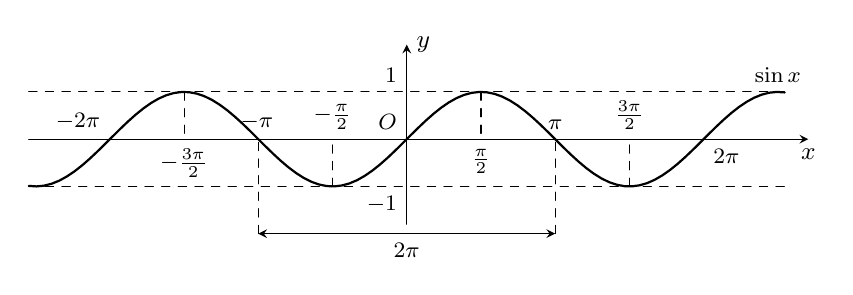
\begin{tikzpicture}[>=stealth,line join=round,line cap=round,font=\footnotesize,scale=0.6]
					\draw[->] (-8,0) -- (8.5,0) node[below]  {\small $x$};
					\draw[->] (0,-1.8) -- (0,2) node[right] {\small $y$}; 
					\draw[thick,samples=100,domain=-8:8] plot  (\x,{sin ((\x)*180/pi)});
					\draw  (0,0) node [above left] {$O$};
					\draw  (0,1) node [above left] {$1$};
					\draw  (0,-1) node [below left] {$-1$};
					\draw  (-2*pi,0) node[above left] {$-2\pi$};
					\draw (2*pi,0)  node[below right] {$2\pi$};
					 \draw[dashed] (-3*pi/2,1)--(-3*pi/2,0) node[below] {$-\frac{3\pi}{2}$};
					 \draw[dashed] (3*pi/2,-1)--(3*pi/2,0) node[above] {$\frac{3\pi}{2}$};
					\draw  (-3.17,0) node[above] {$-\pi$};
					\draw  (pi,0) node[above] {$\pi$};
					 \draw[dashed] (-pi/2,-1)--(-pi/2,0) node[above] {$-\frac{\pi}{2}$};
					\draw[dashed] (pi/2,1)--(pi/2,0) node[below]  {$\frac{\pi}{2}$};
					\draw[dashed]  (-8,1)--(8,1);
					\draw[dashed]  (-8,-1)--(8,-1);
					\draw[<->] (-pi,-2)--(0,-2) node[below] {$2\pi$}--(pi,-2); 
					 \draw[dashed] (-pi,-2)--(-pi,0);
					 \draw[dashed] (pi,-2)--(pi,0);
					\draw (5*pi/2,1) node[above] {$\sin x$}; 
				\end{tikzpicture}
		\end{center}
		Dựa vào đồ thị trên, ta có bảng  biến thiên của hàm số $y=\sin x$ xét trên đoạn $\left[-\dfrac{\pi}{3};\dfrac{2\pi}{3} \right]$
		\begin{center}
			\begin{tikzpicture}
					 \tkzTabInit[lgt=2,espcl=2]
						{$x$ /  1,$\sin (x)$ / 2}
						{$\dfrac{-\pi}{3}$,$0$,$\dfrac{\pi}{2}$,$\dfrac{2\pi}{3}$} 
					 \tkzTabVar{-/$\frac{-\sqrt{3}}{2}$,R/,+/$1$,-/$\frac{\sqrt{3}}{2}$}
					 \tkzTabIma{1}{3}{2}{0}
				\end{tikzpicture}
		\end{center}
		Dựa vào bảng biến thiên, ta thấy tập giá trị của hàm số là  $T=\left[-\dfrac{\sqrt{3}}{2};1\right]$. Vậy $M=1$ và $m=\dfrac{\sqrt{3}}{2}$ nên $M^2+m^2=1,75$.
	} 
\end{ex}

% nguồn: Ok_TraLoiNgan_Lop11_Lan2
\begin{ex}%[1D1H4-6]%[ma:acd330ee]
	Hàm số $y=\sin \left(x+\dfrac{\pi}{3} \right)-\sin x$ có tất cả bao nhiêu giá trị nguyên? 
	\shortans{3} 
	\loigiai{ 
		Hàm số có tập xác định  $\mathscr{D}=\mathbb{R}$. \\
		Áp dụng công thức $\sin a-\sin b=2\cos \dfrac{a+b}{2}  \sin \dfrac{a-b}{2}$, ta có
		 \[\sin \left(x+\dfrac{\pi}{3} \right)-\sin x=2\cos \left(x+\dfrac{\pi}{6} \right)\sin \dfrac{\pi}{6}=\cos \left(x+\dfrac{\pi}{6} \right).\]
		Ta có $-1\le  \cos \left(x+\dfrac{\pi}{6} \right)\le 1\Leftrightarrow -1\le y\le 1$.\\
		Mà $y\in \mathbb{Z}$  nên $y\in \left\{-1;0;1\right\}$. \\
		Vậy có $3$ giá trị thỏa  mãn.
	} 
\end{ex}

% nguồn: Ok_TraLoiNgan_Lop11_Lan2
\begin{ex}%[1D1H4-6]%[ma:55f16a30]
	Biết rằng tập giá trị của hàm số $y=5+4\sin 2x\cos 2x$ là $T=\left[a; b\right]$. Tính giá trị biểu  thức $P=a+2b$?
	 \shortans{17}
	 \loigiai{
		Hàm số có tập xác định  $\mathscr{D}=\mathbb{R}$. \\
		Ta có $y=5+4\sin 2x\cos 2x=5+2\sin 4x$.\\ 
		Do  \allowdisplaybreaks
		\begin{eqnarray*}
			&&-1\le  \sin 4x\le 1\\
			&\Leftrightarrow& -2\le  2\sin 4x\le 2\\
			&\Leftrightarrow& 3\le 5+2\sin 4x\le 7\\ 
			&\Leftrightarrow&  3\le y\le 7.
		\end{eqnarray*}
		Vậy giá trị của hàm số  là $T=\left[3;7\right]$ nên $\heva{&a=3\\&b=7} \Rightarrow P=a+2b=3+2\cdot 7=17$.
	} 
\end{ex}

% nguồn: Ok_TraLoiNgan_Lop11_Lan2
\begin{ex}%[1D1H4-6]%[ma:cd10ecef]
	 Hàm số $y=5+4\sin 2x\cos 2x$ có tất cả bao nhiêu giá trị nguyên?
	 \shortans{5}
	\loigiai{ 
		Hàm số có  tập xác định $\mathscr{D}=\mathbb{R}$. \\
		Ta có $y=5+4\sin 2x\cos  2x=5+2\sin 4x$.\\
		 Mà \allowdisplaybreaks
		\begin{eqnarray*}
			 &&-1\le \sin 4x\le 1\\
			&\Leftrightarrow& -2\le 2\sin 4x\le  2\\
			&\Leftrightarrow& 3\le 5+2\sin  4x\le 7\\
			 &\Leftrightarrow& 3\le y\le 7.
		\end{eqnarray*}
		Mà $y\in \mathbb{Z}$ nên $y\in  \left\{3;4;5;6;7\right\}$. \\
		Vậy có $5$ giá trị  thỏa mãn.
	 }
\end{ex}

% nguồn: Ok_TraLoiNgan_Lop11_Lan2
\begin{ex}%[1D1H4-6]%[ma:d2e15d86]
	Biết rằng  tập giá trị của hàm số $y=\sin x+\sqrt{3} \cos x+3$ là $T=\left[a; b\right]$. Tính giá trị biểu thức $P=5a+2b$?
	 \shortans{15}
	 \loigiai{
		Hàm số có  tập xác định $\mathscr{D}=\mathbb{R}$.\\
		 Ta có \allowdisplaybreaks
		\begin{eqnarray*}
			 y=\sin x+\sqrt{3} \cos x+3&=&2\left(\dfrac{1}{2} \sin x+\dfrac{\sqrt{3}}{2} \cos x\right)+3\\
			&=&2\sin \left(x+\dfrac{\pi}{3} \right)+3. 
		\end{eqnarray*}
		Do  \allowdisplaybreaks
		\begin{eqnarray*}
			&&-1\le \sin \left(x+\dfrac{\pi}{3}  \right)\le 1\\
			&\Leftrightarrow& -2\le 2\sin  \left(x+\dfrac{\pi}{3} \right)\le 2\\
			&\Leftrightarrow& 1\le 2\sin \left(x+\dfrac{\pi}{3} \right)+3\le 5\\ 
			 &\Leftrightarrow& 1\le y\le 5.
		\end{eqnarray*}
		Vậy giá trị của  hàm số là $T=\left[1; 5\right]$ nên $\heva{&a=1\\&b=5} \Rightarrow P=5a+2b=5\cdot 1+2\cdot 5=15$.
	} 
\end{ex}

% nguồn: Ok_TraLoiNgan_Lop11_Lan2
\begin{ex}%[1D1H4-6]%[ma:2bf4c7ed]
	Biết rằng tập giá trị của hàm số $y=\cos ^2x+2\sin x+2$ là  $T=\left[a; b\right]$. Tính giá trị biểu thức $P=10a-2b$?
	 \shortans{-8}
	\loigiai{ 
		Hàm số có tập xác  định $\mathscr{D}=\mathbb{R}$.\\
		 Ta có \allowdisplaybreaks
		\begin{eqnarray*}
			 y=\cos ^2x+2\sin x+2&=&\left(1-\sin ^2x\right)+2\sin x+2\\
			&=&-\sin  ^2x+2\sin x+3\\
			 &=&-\left(\sin x-1\right)^2+4.
		\end{eqnarray*}
		 Do \allowdisplaybreaks
		\begin{eqnarray*}
			&&-1\le \sin x\le  1\\
			 &\Leftrightarrow& -2\le \sin x-1\le 0\\
			&\Leftrightarrow& 4\ge \left(\sin  x-1\right)^2\ge 0\\
			 &\Leftrightarrow& 4\le-\left(\sin x-1\right)^2\le 0\\
			&\Leftrightarrow& 0\le-\left(\sin x-1\right)^2+4\le 4\\ 
			&\Leftrightarrow& 0\le y\le 4. 
		\end{eqnarray*}
		Vậy giá trị của hàm số là $T=\left[0; 4\right]$ nên $\heva{&a=0\\&b=4}  \Rightarrow P=10a-2b=10\cdot 0-2\cdot 4=-8$.
	} 
\end{ex}

% nguồn: Ok_TraLoiNgan_Lop11_Lan2
\begin{ex}%[1D1H4-6]%[ma:a5e26157]
	Biết rằng tập giá trị của hàm số $y=\sin ^6x+\cos ^6x$ là $T=\left[a; b\right]$. Tính giá trị biểu  thức $P=4a+b$.
	\shortans{2} 
	\loigiai{ 
		Hàm số  có tập xác định $\mathscr{D}=\mathbb{R}$.\\
		 Ta có \allowdisplaybreaks
		\begin{eqnarray*}
			y=\sin ^6x+\cos ^6x&=&\left(\sin ^2x+\cos ^2x\right)^3-3\sin  ^2x\cos ^2x\left(\sin ^2x+\cos ^2x\right)\\
			&=&1-\dfrac{3}{4} \sin  ^22x.
		\end{eqnarray*}
		Do  \allowdisplaybreaks
		\begin{eqnarray*}
			&&0\le  \sin ^22x\le 1\\
			&\Leftrightarrow& 0\ge-\dfrac{3}{4} \sin ^22x\ge-\dfrac{3}{4}\\  &\Leftrightarrow& 1\ge 1-\dfrac{3}{4} \sin ^22x\ge \dfrac{1}{4}\\ &\Leftrightarrow& 1\ge y\ge \dfrac{1}{4}.
		\end{eqnarray*}
		Vậy giá trị của hàm số là $T=\left[\dfrac{1}{4};1\right]$ nên  $\heva{&a=\dfrac{1}{4}\\&b=1} \Rightarrow P=4a+b=4\cdot\dfrac{1}{4}+1=2$.
	 }
\end{ex}

% nguồn: Ok_TraLoiNgan_Lop11_Lan2
\begin{ex}%[1D1H4-6]%[ma:cff3d2f7]
	Tập giá trị của hàm số $y=5+4\sin 2x \cos 2x$ là  $[a; b]$. Tính $b-a$.
	 \shortans{4}
	\loigiai{ 
		Hàm số có tập  xác định $\mathscr{D}=\mathbb{R}$. \\
		Ta có  $y=5+4\sin 2x \cos 2x=5+2\sin 4x$. \\
		Do $-1\leq \sin 4x \leq 1\Leftrightarrow-2\leq 2\sin 4x \leq 2\Leftrightarrow 3\leq 5+2\sin 4x \leq 7\Leftrightarrow 3\leq  y \leq 7$. \\
		Từ đó giá trị của hàm số là $T=[3; 7]$. \\ 
		Vậy  $b-a=7-3=4$.
	} 
\end{ex}

% nguồn: Ok_TraLoiNgan_Lop11_Lan2
\begin{ex}%[1D1H4-6]%[ma:cacd4971]
	Hàm số $y=\cos ^2x-\cos x$ có tất cả bao  nhiêu giá trị nguyên?
	\shortans{3} 
	\loigiai{ 
		 Hàm số có tập xác định $\mathscr{D}=\mathbb{R}$. \\
		Ta  có $y=\cos ^2x-\cos x=\left(\cos x-\dfrac{1}{2} \right)^2-\dfrac{1}{4}$.\\
		 Mà \allowdisplaybreaks
		\begin{eqnarray*}
			&&-1\le \cos x\le 1\\ 
			&\Leftrightarrow& -\dfrac{3}{2}  \le \cos x-\dfrac{1}{2} \le \dfrac{1}{2}\\
			&\Leftrightarrow& 0\le \left(\cos x-\dfrac{1}{2} \right)^2\le  \dfrac{9}{4}\\
			&\Leftrightarrow& -\dfrac{1}{4}  \le \left(\cos x-\dfrac{1}{2} \right)^2-\dfrac{1}{4} \le 2\\
			&\Leftrightarrow& -\dfrac{1}{4} \le y\le  2.
		\end{eqnarray*}
		Mà $y\in \mathbb{Z}$ nên  $y\in \left\{0;1;2\right\}$. \\
		Vậy  có $3$ giá trị thỏa mãn.
	} 
\end{ex}

% nguồn: Ok_TraLoiNgan_Lop11_Lan2
\begin{ex}%[1D1H4-6]%[ma:b62343e5]
	Tập giá trị của hàm số $y=\sin x$ trên đoạn $\left[-\dfrac{\pi}{3}; \dfrac{2 \pi}{3}\right]$ là tập $S$. Số nguyên lớn nhất thuộc tập $S$ là bao  nhiêu?
	\shortans{1} 
	\loigiai{ 
		Xét hàm số $y=\sin x$ trên đoạn  $\left[-\dfrac{\pi}{3}; \dfrac{2 \pi}{3}\right]$. \\
		Ta có đồ thị của hàm  số $y=\sin x$ trên $\mathbb{R}$ như sau
		\begin{center}
			\begin{tikzpicture}[line join = round,line cap = round,>=stealth,thick,scale = 1]
					\draw[->,line width = 1pt] (-8,0)--(0,0)  node[below right]{$O$}--(8,0) node[below]{$x$};
					\draw[->,line width = 1pt]  (0,-2)--(0,2) node[left]{$y$};
					\fill (0,0)  circle (1.5pt);
					\begin{scope}
						\clip (-8,-2) rectangle  (8,2);
						\draw[samples=300,domain=-8:8,smooth,blue!50!black]  plot (\x,{sin (\x r)});
					\end{scope}
					\foreach \x in {-2*pi,-1.5*pi,-pi,-.5*pi,.5*pi,pi,1.5*pi,2*pi} \draw[thin] (\x,2pt)--(\x,-2pt); 
					\foreach \y in {-1,1} \draw[thin] (2pt,\y)--(-2pt,\y) node [left] {$\y$}; 
					\node at (-pi,0) [above] {$-\pi$}; 
					\node  at (pi,0) [above] {$\pi$};
					\node at (-2*pi,0)  [below] {$-2\pi$};
					\node at (2*pi,0)  [below] {$2\pi$};
					\draw[dashed]  (-1.5*pi,0) node [below] {$-\dfrac{3\pi}{2}$}--(-1.5*pi,1);
					\draw[dashed] (-.5*pi,0) node[above] {$-\dfrac{\pi}{2}$}--(-.5*pi,-1); 
					\draw[dashed] (.5*pi,0) node [below] {$\dfrac{\pi}{2}$}--(.5*pi,1); 
					\draw[dashed]  (-2.5*pi,1)--(2.5*pi,1)
						 (-2.5*pi,-1)--(2.5*pi,-1);
					\draw[dashed] (1.5*pi,0) node [above]  {$\dfrac{3\pi}{2}$}--(1.5*pi,-1);
					\node[red] at (7,1)  [above] {$y = \sin x$};
				\end{tikzpicture}
		\end{center}
		Dựa vào đồ thị trên,  ta có bảng biến thiên của hàm số $y=\sin x$ xét trên đoạn $\left[-\dfrac{\pi}{3}; \dfrac{2 \pi}{3}\right]$ là
		\begin{center}
			\begin{tikzpicture}
					 \tkzTabInit[nocadre,lgt=2,espcl=3,deltacl=0.5]
						{$x$/1,$\sin x$/2.5} 
						{$-\dfrac{\pi}{3}$,$0$,$\dfrac{\pi}{2}$,$\dfrac{2\pi}{3}$} 
					\draw (N12)  node[above](A){$-\dfrac{\sqrt{3}}{2}$}
						($(N12)!0.5!(N31)$) node  (B){$0$}
						 (N31)
						node[below](C){$1$} 
						(N42) node[above](D){$\dfrac{\sqrt{3}}{2}$}; 
					\draw[-stealth] (A)--(B); 
					\draw[-stealth]  (B)--(C);
					\draw[-stealth]  (C)--(D);
				\end{tikzpicture}
		\end{center}
		Dựa vào bảng biến thiên,  ta thấy tập giá trị của hàm số là $T=\left[-\dfrac{\sqrt{3}}{2}; 1\right]$. \\
		Suy ra số  nguyên lớn nhất thuộc tập $S$ là $1$.
	} 
\end{ex}

% nguồn: Ok_TraLoiNgan_Lop11_Lan2
\begin{ex}%[1D1H4-6]%[ma:4ac752a3]
	Tập giá trị của hàm số $y=\sin x+\sqrt{3}\cos x+3$  là $[a; b]$. Tính $a+b$.
	\shortans{6} 
	\loigiai{ 
		Ta  có $y=\sin x+\sqrt{3}\cos x+3=2\left(\dfrac{1}{2}\sin x+\dfrac{\sqrt{3}}{2}\cos x\right)+3=2\sin \left(x+\dfrac{\pi}{3}\right)+3$. \\
		Do $-1\leq \sin  \left(x+\dfrac{\pi}{3}\right)\leq 1\Leftrightarrow-2\leq 2\sin \left(x+\dfrac{\pi}{3}\right)\leq 2\Leftrightarrow 1\leq 2\sin \left(x+\dfrac{\pi}{3}\right)+3\leq 5\Leftrightarrow 1\leq y \leq 5$. \\
		Từ đó có tập giá trị của hàm số là  $T=[1; 5]$. \\
		Vậy $a+b=1+5=6$. 
	} 
\end{ex}

% nguồn: Ok_TraLoiNgan_Lop11_Lan2
\begin{ex}%[1D1H4-6]%[ma:743f28a7]
	Tập giá trị của hàm số $y=\sin ^6x+\cos ^6x$ là $\left[\dfrac{1}{4}; 1\right]$. Tính  $8a\cdot b$.
	 \shortans{2}
	\loigiai{ 
		Hàm số có  tập xác định $\mathscr{D}=\mathbb{R}$. \\
		Ta  có
		$$ 
		y=\sin ^6 x+\cos ^6  x=\left(\sin ^2 x+\cos ^2 x\right)^3-3 \sin ^2 x \cos ^2 x\left(\sin ^2 x+\cos ^2 x\right)=1-\dfrac{3}{4}\sin ^2 2 x
		$$ 
		Do $0\leq \sin ^22x \leq 1\Leftrightarrow 0\geq-\dfrac{3}{4}\sin ^22x \geq-\dfrac{3}{4}\Leftrightarrow 1\geq  1-\dfrac{3}{4}\sin ^22x \geq \dfrac{1}{4}\Leftrightarrow 1\geq y \geq \dfrac{1}{4}$. \\
		Từ đó có tập giá trị của hàm số là $T=\left[\dfrac{1}{4}; 1\right]$. \\ 
		Vậy $8a\cdot b=8\cdot \dfrac{1}{4}\cdot  1=2$.
	 }
\end{ex}

% nguồn: Ok_TraLoiNgan_Lop11_Lan1
\begin{ex}%[1D1V4-6]%[ma:4031b8d3]
	Số giờ có ánh sáng mặt trời của một thành phố tại vĩ độ $40^\circ$ Bắc trong ngày thứ $t$ của năm được cho bởi hàm số  $d(t) = 4 \sin\left[\dfrac{\pi}{182}(t - 88)\right] + 10$ (giờ), với $t$ là số ngày trong năm từ $1$ đến $365$. Ngày đầu tiên tạo $10$ giờ ánh sáng mặt trời là ngày.
	\shortans{88} 
	 \loigiai{
		Với $t\in[1;365]$ ta có 
		\begin{eqnarray*}
			& & \sin\left[\dfrac{\pi}{182}(t - 88)\right] + 10  = 10\\
			&\Leftrightarrow &  \sin\left[\dfrac{\pi}{182}(t - 88)\right] = 0\\
			&\Leftrightarrow &  \dfrac{\pi}{182}(t - 88)=k\pi\\
			&\Leftrightarrow  & t=88+182k\\
			&\Leftrightarrow  & t \in \{88, 270\}.
		\end{eqnarray*}
	Số ngày tạo $10$ giờ ánh  sáng mặt trời ngày đầu tiên của năm là $88$.}
\end{ex}

% nguồn: Ok_TraLoiNgan_Lop11_Lan2
\begin{ex}%[1D1V4-6]%[ma:45bab352]
	Tìm $m$ để giá trị lớn nhất của hàm số  $y=3\sin x+4\cos x+m$ bằng $10$.
	\shortans{5} 
	\loigiai{ 
		Ta có  phương trình $3\sin x+4\cos x+m=y$ có nghiệm khi và chỉ khi
		 \allowdisplaybreaks
		\begin{eqnarray*} &&{3^2}+4^2\geq{\left(y-m\right)^2}\\
			 &\Leftrightarrow&-5\le{y}-m\leq 5\\ &\Leftrightarrow&-5+m\le{y}\leq 5+m.
		\end{eqnarray*}
	Theo giả  thiết $\max y=5+m=10\Leftrightarrow 10=5+m\Leftrightarrow m=5$.}
\end{ex}

% nguồn: Ok_TraLoiNgan_Lop11_Lan2
\begin{ex}%[1D1V4-6]%[ma:9ea680b3]
	 Giá trị lớn nhất và giá trị nhỏ nhất của hàm số $y=\sin ^2 x+\sin x-3$ lần lượt là $M$ và $N$. Tìm $M-N$.
	 \shortans{9}
	 \loigiai{
		Đặt $t=\sin x,  t \in[-1; 1]$. Ta có $y=t^2+t-3$. \\
		Đây là hàm bậc hai với $a=1$, $b=1$, suy ra $-\dfrac{b}{2  a}=-\dfrac{1}{2}$. \\
		Vì $a>0$ nên  bề lõm parabol tương ứng sẽ hướng lên trên. \\
		Bảng biến  thiên
		\begin{center}
			\begin{tikzpicture}
					 \tkzTabInit[nocadre=true,lgt=1.2,espcl=4,deltacl=0.5]
						{$t$/0.7,$f  (t)$/2}
						{$-\infty$,$-\tfrac{1}{2}$,$+\infty$} 
					\tkzTabVar{+/$+\infty$,-/$-\-\dfrac{13}{4}$,+/$+\infty$} 
					\tkzTabVal[draw]{2}{3}{0.5}{$1$}{$-1$} 
					\tkzTabVal[draw]{1}{2}{0.5}{$-1$}{$-3$} 
					\fill[pattern=north west lines,opacity=0.3] (M21) rectangle (T22); 
					\fill[pattern=north west lines,opacity=0.3] (M11) rectangle (T12); 
				\end{tikzpicture}
		\end{center}
		Dựa vào  bảng biến thiên, ta thấy
		\begin{itemize}
			\item $M=\max\limits_{[-1; 1]}y=-1$ đạt được khi  $t=1 \Leftrightarrow \sin x=1 \Leftrightarrow x=\dfrac{\pi}{2}+k 2 \pi (k \in \mathbb{Z})$.
			\item $N=\min\limits_{[-1; 1]}y=-\dfrac{13}{4}$ đạt được khi  $t=-\dfrac{1}{2}\Leftrightarrow \sin x=-\dfrac{1}{2}\Leftrightarrow\hoac{&x=-\dfrac{\pi}{6}+k 2 \pi \\ &x=\dfrac{7 \pi}{6}+k 2 \pi}(k \in \mathbb{Z})$.
		\end{itemize}
		Vậy  $4(M-N)=4\cdot\left(-1-\left(-\dfrac{13}{4}\right)\right)=4\cdot \dfrac{9}{4}=9$.
	} 
\end{ex}

% nguồn: Ok_TraLoiNgan_Lop11_Lan2
\begin{ex}%[1D1V4-6]%[ma:b02d3ddf]
	Tìm giá trị nhỏ nhất của hàm  số $y=1-3\sqrt{1-\cos ^2x}$.
	 \shortans{-2}
	\loigiai{ 
		Ta có\\ 
		$\begin{aligned}
		&\cos  ^2\ge 0\\
		\Rightarrow&-\cos  ^2\le 0\\
		\Rightarrow& 1-\cos  ^2\le 1\\
		\Rightarrow& \sqrt{1-\cos  ^2}\le 1\\
		\Rightarrow&-3\sqrt{1-\cos  ^2}\ge-3\\
		 \Rightarrow& 1-3\sqrt{1-\cos ^2}\ge-2\\
		\Rightarrow&  y\ge-2.
	\end{aligned}$\\
	 Khi đó\\
	$\begin{aligned}
	 &y=-2\\
	\Leftrightarrow&  1-\cos ^2x=1\\
	\Leftrightarrow& \cos ^2x=0\\ 
	 \Leftrightarrow& \cos x=0\\
	\Leftrightarrow &x=\dfrac{\pi}{2}+k\pi, k\in  \mathbb{Z}.
	\end{aligned}$\\
	Vậy tại $x=\dfrac{\pi}{2}+k\pi, k\in \mathbb{Z}$ thì  $y$ đạt giá trị nhỏ nhất bằng $-2$.
 }
\end{ex}

% nguồn: Ok_TraLoiNgan_Lop11_Lan2
\begin{ex}%[1D1V4-6]%[ma:594ec4c6]
	Biết giá trị lớn nhất của hàm số $y=\sin^4x+\cos^4x+\sin x\cos x$ đạt được bằng $\dfrac{a}{b}$ với $a$, $b\in\mathbb{N}$, $\dfrac{a}{b}$ là phân số  tối giản. Tổng $a+b$ bằng bao nhiêu?
	\shortans{17} 
	\loigiai{\allowdisplaybreaks 
		\begin{eqnarray*}
			y&=&\sin^4x+\cos^4x+\sin  x\cos x\\ &=&\left(\sin^2x+\cos^2x\right)^2-2\left(\sin x\cdot\cos x\right)^2+\sin x\cos x\\
			&=&1-2\cdot\dfrac{1}{4}{\sin^2}2x+\dfrac{1}{2}\sin  2x.
		\end{eqnarray*}
		Đặt $t=\sin 2x\in[-1;1]$. 
		Khi  đó $f(t)=-\dfrac{1}{2}t^2+\dfrac{1}{2}t+1$, $t\in\left[-1;1\right]$.\\
		Ta có hoành độ đỉnh $t_0=\dfrac{1}{2}\in[-1;1]$  mà $y\left(-1\right)=0$; $y(1)=1$; $y\left(\dfrac{1}{2}\right)=\dfrac{9}{8}$.\\
	Suy ra giá trị lớn  nhất là $\dfrac{9}{8}$ đạt được khi $\sin 2x=\dfrac{1}{2}$ suy ra $\dfrac{a}{b}=\dfrac{9}{8}\Rightarrow a+b=17$.}
\end{ex}

% nguồn: Ok_TraLoiNgan_Lop11_Lan2
\begin{ex}%[1D1V4-6]%[ma:c1743cb1]
	Biết giá trị lớn nhất và giá trị nhỏ nhất của hàm số  $y=3\sin ^2\left(3x+\dfrac{\pi}{6}\right)+4$ lần lượt là $M$ và $m$. Tính $m+M$.
	 \shortans{11}
	 \loigiai{
		Ta có\\ 
		$\begin{aligned}
		&-1\le  \sin \left(3x+\dfrac{\pi}{6}\right)\le 1, \forall x\in \mathbb{R}\\
		\Rightarrow &0\le \sin ^2\left(3x+\dfrac{\pi}{6}\right)\le  1, \forall x\in \mathbb{R}\\
		\Rightarrow  & 4\le 3\sin ^2\left(3x+\dfrac{\pi}{6}\right)+4\le 7, \forall x\in \mathbb{R}\\
		 \Rightarrow & 4\le y\le 7, \forall x\in \mathbb{R}.
	\end{aligned}$\\
	 Suy ra $m=y_{\min}=4$ và $M=y_{\max}=7$. \\
	 Vậy $m+M=4+7=11$.
} 
\end{ex}

% nguồn: Ok_TraLoiNgan_Lop11_Lan2
\begin{ex}%[1D1V4-6]%[ma:14a4b65a]
	 Biết giá trị lớn nhất và giá trị nhỏ nhất của hàm số $y=2+2\cos x+\cos ^2x$ lần lượt là $M$ và $m$. Tính $3M+m$.
	\shortans{16} 
	 \loigiai{
		Ta có  $y=2+2\cos x+\cos ^2x=(\cos x+1)^2+1$. \\
		 Khi đó\\
		$\begin{aligned}
		 &-1\le \cos x\le 1, \forall x\in \mathbb{R}\\
		&\Rightarrow 0\le 1+\cos x\le 2, \forall x\in  \mathbb{R}\\
		&\Rightarrow 1\le (1+\cos x)^2+1\le  5, \forall x\in \mathbb{R}\\
		&\Rightarrow 1\le y\le 5,  \forall x\in \mathbb{R}.
	\end{aligned}$
	\begin{itemize}
		\item  Ta có\\
		$\begin{aligned}
		&M=\max{y}=5\\ 
		 &\Leftrightarrow \cos x=1\\
		&\Leftrightarrow  x=k2\pi, k\in \mathbb{Z}.
	\end{aligned}$
	\item  Ta có\\
	$\begin{aligned}
	 &m=\min{y}=1\\
	&\Leftrightarrow  \cos x=-1\\
	 &\Leftrightarrow x=\pi+k2\pi, k\in \mathbb{Z}.
	\end{aligned}$
	\end{itemize}
	Vậy  $3M+m=3\cdot 5+1=16$.
 }
\end{ex}

% nguồn: Ok_TraLoiNgan_Lop11_Lan2
\begin{ex}%[1D1V4-6]%[ma:c149a3f7]
	Với giá trị nào của $m$ thì hàm số $y=\sin 3x-\cos 3x+m$ có giá trị lớn nhất bằng  $\sqrt{2}$.
	 \shortans{0}
	 \loigiai{
		Ta có  $y=\sin 3x-\cos 3x+m=\sqrt{2}\left(\dfrac{1}{\sqrt{2}}\sin 3x-\dfrac{1}{\sqrt{2}}\text{cos3}x\right)+m=\sqrt{2}\sin\left(3x-\dfrac{\pi}{4}\right)+m\le\sqrt{2}+m$.\\
	Do đó giá trị lớn nhất  của $y$ bằng $\sqrt{2}$ khi $\sqrt{2}+m=\sqrt{2}\Leftrightarrow m=0.$}
\end{ex}

% nguồn: Ok_TraLoiNgan_Lop11_Lan2
\begin{ex}%[1D1V4-6]%[ma:047cf762]
	Biết giá trị lớn nhất và giá trị nhỏ nhất của hàm số $y=2\cos \left(x-\dfrac{\pi}{3}\right)-1$ lần lượt là  $M$ và $m$. Tính $2M+3m$.
	 \shortans{-7}
	 \loigiai{
		Tập xác định $\mathscr{D}=\mathbb{R}$. \\ 
		Ta có\\ 
		$\begin{aligned}
		&-1\le \cos \left(x-\dfrac{\pi}{3}\right)\le 1,  \forall x\in \mathbb{R}\\
		 \Leftrightarrow &-2\le 2\cos \left(x-\dfrac{\pi}{3}\right)\le 2, \forall x\in \mathbb{R}\\
		\Leftrightarrow &-3\le  2\cos \left(x-\dfrac{\pi}{3}\right)-1\le 1, \forall x\in \mathbb{R}.
	\end{aligned}$\\
	\begin{itemize}
		\item Ta có\\ 
		$\begin{aligned}
		 &M=\max{y}=1\\
		&\Leftrightarrow  \cos \left(x-\dfrac{\pi}{3}\right)=1\\
		 &\Leftrightarrow x-\dfrac{\pi}{3}=k2\pi \\
		&\Leftrightarrow x=\dfrac{\pi}{3}+k2\pi, k\in  \mathbb{Z}.
	\end{aligned}$\\
	 \item Ta có\\
	$\begin{aligned}
	 &m=\min{y}=-3\\
	&\Leftrightarrow \cos  \left(x-\dfrac{\pi}{3}\right)=-1\\
	&\Leftrightarrow  x-\dfrac{\pi}{3}=\pi+k2\pi\\
	&\Leftrightarrow x=\dfrac{4\pi}{3}+k2\pi,  k\in \mathbb{Z}.
	\end{aligned}$
	\end{itemize}
	 Vậy $2M+3m=2\cdot 1+3\cdot (-3)=-7$.
 }
\end{ex}

% nguồn: Ok_TraLoiNgan_Lop11_Lan2
\begin{ex}%[1D1V4-6]%[ma:529df2c6]
	Tập giá trị của hàm số $y=\dfrac{2 \sin x+\cos  x}{\sin x+2 \cos x+4}$ là $[a; b]$. Tính $a\cdot b$ (kết quả để ở dạng thập phân, làm tròn đến hàng phần trăm).
	 \shortans{0,46}
	\loigiai{ 
		Tập xác định  hàm số $\mathscr{D}=\mathbb{R}$. \\
		Ta  có
		$$y=\dfrac{2\sin x+\cos x}{\sin x+2\cos x+4}\Leftrightarrow y(\sin x+2\cos x+4)=2\sin x+\cos x\Leftrightarrow(y-2) \sin x+(2y-1) \cos x=-4y.  $$
		Điều kiện để tồn tại cặp $(x;  y)$ là
		$$(y-2)^2+(2y-1)^2\geq(-4y)^2\Leftrightarrow-11y^2-8y+5\geq  0\Leftrightarrow \dfrac{-4-\sqrt{71}}{11}\leq y \leq \dfrac{-4+\sqrt{71}}{11}. $$
		Suy ra tập giá trị hàm số  là $T=\left[\dfrac{-4-\sqrt{71}}{11}; \dfrac{-4+\sqrt{71}}{11}\right]$. \\
		Vậy $a\cdot b=\dfrac{-4-\sqrt{71}}{11}\cdot \dfrac{-4+\sqrt{71}}{11}\approx 0{,}46$. 
	} 
\end{ex}

% nguồn: Ok_TraLoiNgan_Lop11_Lan2
\begin{ex}%[1D1V4-6]%[ma:e23179c8]
	Biết giá trị lớn nhất và giá trị nhỏ nhất của  hàm số $y=\sqrt{1+\sin x}-3$ lần lượt là $M$ và $m$. Tính $M+m-\sqrt{2}$.
	\shortans{-6} 
	\loigiai{ 
		Do $\sin  x\ge-1, \forall x\in \mathbb{R}$ nên tập xác định của hàm số là $\mathscr{D}=\mathbb{R}$. \\
		 Ta có\\
		$\begin{aligned}
		&-1\le \sin x\le 1,  \forall x\in \mathbb{R}\\
		&\Leftrightarrow  0\leq 1+\sin x \leq 2, \forall x \in \mathbb{R}\\
		&\Leftrightarrow-3\leq \sqrt{1+\sin x}-3\leq \sqrt{2}-3, \forall x  \in \mathbb{R}\\
		&\Leftrightarrow-3\leq y \leq \sqrt{2}-3, \forall x \in  \mathbb{R}.
	\end{aligned}$
	\begin{itemize}
		\item Ta  có\\
		$\begin{aligned}
		&M=\max{y}=\sqrt{2}-3\\ 
		&\Leftrightarrow \sin  x=1\\
		&\Leftrightarrow x=\frac{\pi}{2}+k2\pi,  k \in \mathbb{Z}.
	\end{aligned}$
	\item Ta  có\\
	$\begin{aligned}
	&m=\min{y}=-3\\ 
	&\Leftrightarrow \sin  x=-1\\
	&\Leftrightarrow x=-\frac{\pi}{2}+k2\pi, k \in  \mathbb{Z}.
	\end{aligned}$
	\end{itemize}
	Vậy  $M+m-\sqrt{2}=\sqrt{2}-3-3-\sqrt{2}=-6$.
 }
\end{ex}

% nguồn: Ok_TraLoiNgan_Lop11_Lan2
\begin{ex}%[1D1V4-6]%[ma:f52e148a]
	Tập  giá trị của hàm số $y=\cos ^2x+2\sin x+2$ là $[a; b]$. Tính $a^2+b^2$.
	 \shortans{16}
	\loigiai{ 
		Hàm  số có tập xác định $\mathscr{D}=\mathbb{R}$. \\
		Ta có $y=\cos ^2x+2\sin x+2=\left(1-\sin ^2x\right)+2\sin x+2=-\sin ^2x+2\sin x+3=-(\sin x-1)^2+4$.  \\
		Lại có 
		\begin{eqnarray*}-1\leq \sin x \leq 1&\Leftrightarrow&-2\leq \sin x-1\leq 0\Leftrightarrow 4\geq(\sin x-1)^2\geq 0\\
			&\Leftrightarrow& 4\leq-(\sin  x-1)^2\leq 0\Leftrightarrow 0\leq-(\sin x-1)^2+4\leq 4\Leftrightarrow 0\leq y \leq 4.
		\end{eqnarray*}
		Từ  đó có tập giá trị của hàm số là $T=[0; 4]$. \\
		Vậy  $a^2+b^2=0^2+4^2=16$.
	 }
\end{ex}

% nguồn: Ok_TraLoiNgan_Lop11_Lan2
\begin{ex}%[1D1V4-6]%[ma:3daa71a4]
	Biết giá trị lớn nhất và giá trị nhỏ nhất của hàm số $y=\sin  x+\cos x$ lần lượt là $M$ và $m$. Tính $m+M$.
	\shortans{0} 
	\loigiai{ 
		Ta có\\ 
		$\begin{aligned}
		y=&\sin x+\cos x\\=&\sqrt{2}\sin  x\cdot \cos \dfrac{\pi}{4}+\sqrt{2}\cos x\cdot \sin \dfrac{\pi}{4}\\=&\sqrt{2}\sin \left(x+\dfrac{\pi}{4}\right).
	\end{aligned}$\\
	Khi  đó\\
	$\begin{aligned}
	&-1\le \sin \left(x+\dfrac{\pi}{4}\right)\le 1, \forall x \in \mathbb{R}\\ 
	\Rightarrow&-\sqrt{2}\le \sqrt{2}\sin \left(x+\dfrac{\pi}{4}\right)\le \sqrt{2}, \forall x \in  \mathbb{R}\\
	\Rightarrow&-\sqrt{2}\le y\le \sqrt{2},  \forall x \in \mathbb{R}.
	\end{aligned}$\\
	Suy ra $m=y_{min\;}=-\sqrt{2}$ và $M=y_{\max}=\sqrt{2}$.  \\
	Vậy $m+M=-\sqrt{2}+\sqrt{2}=0$. 
 }
\end{ex}

% nguồn: Ok_TraLoiNgan_Lop11_Lan1
\begin{ex}%[1D1C4-6]%[ma:150ef4c5]
	Tìm tổng giá trị lớn nhất và giá trị nhỏ nhất của  hàm số $y=\dfrac{2\sin x+3\cos x+1}{\sin x-\cos x+2}$
	 \shortans{3}
	\loigiai{ 
		Lý thuyết: $a\sin x +b \cos  x =c$. Phương trình có nghiệm khi $a^2+b^2 \ge c^2$.\\
		 Ta có: $y=\dfrac{2 \sin x+3 \cos x+1}{\sin x-\cos x+2} \Leftrightarrow(y-2) \sin x-(y+3) \cos x=1-2 y$.\\
		Điều kiện để tồn tại  cặp số $(x; y)$ là\\ $(y-2)^2+(y+3)^2 \geq(1-2 y)^2$ $\Leftrightarrow-2 y^2+6 y+12 \geq 0 \Leftrightarrow \dfrac{3-\sqrt{33}}{2} \leq y \leq \dfrac{3+\sqrt{33}}{2}$.\\
		 Tổng giá trị lớn nhất và giá trị nhỏ nhất của hàm số: $\dfrac{3-\sqrt{33}}{2}+\dfrac{3+\sqrt{33}}{2}=3$.
	 }
\end{ex}

% nguồn: Ok_TraLoiNgan_Lop11_Lan1
\begin{ex}%[1D1C4-6]%[ma:362c8e5b]
	Giá trị lớn nhất của hàm số $y=\left(\sin 2x-\cos 2x\right)^2+\cos 4x$  (làm tròn đến hàng phần chục).
	 \shortans{2,4}
	 \loigiai{
		Ta có 
		 \allowdisplaybreaks
		\begin{eqnarray*}
			y&=&\left(\sin 2x-\cos 2x\right)^2+\cos 4x\\ 
			&=&\sin ^22x-2\sin 2x\cos  2x+\cos ^22x+\cos4x\\
			&=&\sin ^22x+\cos  ^22x-2\sin 2x\cos 2x+\cos 4x\\
			 &=&1-\sin 4x+\cos 4x\\
			&=&1-\sqrt{2}\left(\sin  4x\cos \dfrac{\pi}{4}+\cos 4x\sin\dfrac{\pi}{4} \right)\\
			&=&1-\sqrt{2} \sin \left(4x+\dfrac{\pi}{4}  \right).
		\end{eqnarray*}
		Vì $\sin \left(4x+\dfrac{\pi}{4} \right)\in  \left[-1;1\right]$
		nên $1-\sqrt{2}\le y\le 1+\sqrt{2}$.  \\
		Khi $\sin \left(4x+\dfrac{\pi}{4}  \right)=-1\Leftrightarrow 4x+\dfrac{\pi}{4}=-\dfrac{\pi}{2}+k2\pi \Leftrightarrow x=-\dfrac{3\pi}{16}+\dfrac{k\pi}{2} \left(k\in \mathbb{Z}\right)$.\\
		Vậy $y_{\text{max}}=1+\sqrt{2}\approx 2{,}4$. 
	 }
\end{ex}


%%%%%%%%%%%%%%%% TỰ LUẬN %%%%%%%%%%%%%%%%

% nguồn: Ok_TuanLuan_Toan11_Lan2
\begin{ex}%[1D1H4-6]%[ma:b972812e]
	Tìm giá trị lớn nhất, giá trị nhỏ nhất của hàm số sau đây: 
	\begin{enumEX}{2}
		\item $y=2\sin\left(x+\dfrac{\pi}{4}\right)+1$; 
		\item $y=2\sqrt{\cos  x+1}-3$;
		 \item $y=\sin x+\cos x$;
		\item $y=\sqrt{3}\sin  2x-\cos 2x$;
		\item $y=\cos^2x+2\sin x+2$; 
		 \item $y=\sin^4x-2\cos^2x+1$.
	\end{enumEX}
	\loigiai{ 
		\begin{enumerate}
			 \item Ta có \allowdisplaybreaks
			\begin{eqnarray*}
				&&-1 \leq  \sin\left(x+\dfrac{\pi}{4}\right) \leq 1 \\
				 &\Rightarrow& -2 \leq 2\sin\left(x+\dfrac{\pi}{4}\right) \leq 2 \\
				&\Rightarrow& -1 \leq  2\sin\left(x+\dfrac{\pi}{4}\right)+1 \leq 3\\
				&\Rightarrow&-1 \leq  y \leq 3.
			\end{eqnarray*}
			\begin{itemize}
				\item $\max y=3$ khi  $\sin\left(x+\dfrac{\pi}{4}\right)=1\Leftrightarrow x=\dfrac{\pi}{4}+k2\pi,\, k\in\mathbb{Z}$.
				\item $\min y=-1$ khi $\sin\left(x+\dfrac{\pi}{4}\right)=-1\Leftrightarrow x=-\dfrac{3\pi}{4}+k2\pi,\,  k\in\mathbb{Z}$.
			\end{itemize}
			 \item Ta có\allowdisplaybreaks
			\begin{eqnarray*}
				&&-1 \leq \cos x \leq 1 \\ 
				&\Rightarrow& 0 \leq  \cos x+1 \leq 2 \\
				&\Rightarrow& 0  \leq \sqrt{\cos x+1} \leq \sqrt{2}\\
				&\Rightarrow& 0 \leq 2\sqrt{\cos x+1} \leq 2\sqrt{2}\\  &\Rightarrow& -3 \leq 2\sqrt{\cos x+1}-3 \leq 2\sqrt{2}-3\\
				&\Rightarrow&-3 \leq y  \leq 2\sqrt{2}-3.
			\end{eqnarray*}
			\begin{itemize}
				\item $\max y=2\sqrt{2}-3$ khi  $\cos x=1\Leftrightarrow x=k2\pi,\,k\in\mathbb{Z}$.
				\item  $\min y=-3$ khi $\cos x=-1\Leftrightarrow x=\pi+k2\pi,\,k\in\mathbb{Z}$.
			\end{itemize}
			\item Ta  có $y=\sin x+\cos x=\sqrt{2}\sin\left(x+\dfrac{\pi}{4}\right)\Rightarrow-\sqrt{2}\leq y\leq\sqrt{2}$.
			\begin{itemize}
				\item $\max y=\sqrt{2}$ khi $\sin\left(x+\dfrac{\pi}{4}\right)=1\Leftrightarrow x=\dfrac{\pi}{4}+k2\pi,\,k\in\mathbb{Z}$. 
				\item  $\min y=-\sqrt{2}$ khi $\sin\left(x+\dfrac{\pi}{4}\right)=-1\Leftrightarrow x=-\dfrac{3\pi}{4}+k2\pi,\,k\in\mathbb{Z}$.
			\end{itemize}
			\item Ta  có $y=\sqrt{3}\sin 2x-\cos 2x=2\left(\dfrac{\sqrt{3}}{2}\sin 2x-\dfrac{1}{2}\cos 2x\right)=2\sin\left(2x-\dfrac{\pi}{6}\right)\Rightarrow-2\leq y\leq 2$.
			\begin{itemize}
				\item $\max y=2$ khi $\sin\left(2x-\dfrac{\pi}{6}\right)=1\Leftrightarrow 2x-\dfrac{\pi}{6}=\dfrac{\pi}{2}+k2\pi\Leftrightarrow x=\dfrac{\pi}{3}+k\pi,  k\in\mathbb{Z}$.
				\item $\min y=-2$  khi $\sin\left(2x-\dfrac{\pi}{6}\right)=-1\Leftrightarrow 2x-\dfrac{\pi}{6}=-\dfrac{\pi}{2}+k2\pi\Leftrightarrow x=-\dfrac{\pi}{6}+k\pi, k\in\mathbb{Z}$.
			\end{itemize}
			\item Ta có 
			$y=\cos^2x+2\sin x+2=(1-\sin^2x)+2\sin x+2=-\sin^2x+2\sin x+3=-(\sin x-1)^2+4$.\\ 
			Vì  \allowdisplaybreaks
			\begin{eqnarray*}
				&&-1 \leq \sin x  \leq 1\\
				& \Rightarrow& -2 \leq \sin  x - 1 \leq 0 \\
				&\Rightarrow& 4 \geq (\sin x - 1)^2 \geq  0\\
				 &\Rightarrow &-4 \leq -(\sin x - 1)^2 \leq 0 \\
				&\Rightarrow& 0 \leq -(\sin x  - 1)^2 + 4 \leq 4 \\
				&\Rightarrow& 0 \leq y \leq  4.
			\end{eqnarray*}
			\begin{itemize}
				\item $\max y=4$ khi $\sin  x=1\Leftrightarrow x=\dfrac{\pi}{2}+k2\pi,\,k\in\mathbb{Z}$.
				 \item $\min y=0$ khi $\sin x=-1\Leftrightarrow x=-\dfrac{\pi}{2}+k2\pi,\,k\in\mathbb{Z}$.
			\end{itemize}
			 \item Ta có \allowdisplaybreaks
			\begin{eqnarray*}
				y& =& \sin^4 x - 2\cos^2  x + 1 \\
				&=& (1-\cos^2 x)^2 - 2\cos^2  x + 1\\
				& =& \cos^4 x - 4\cos^2 x + 2  \\
				&=& (\cos^2  x - 2)^2 - 2.
			\end{eqnarray*}
			 Ta có
			\allowdisplaybreaks 
			\begin{eqnarray*}
				&&0 \leq \cos^2 x \leq  1 \\
				&\Rightarrow& -2 \leq \cos^2 x - 2 \leq -1  \\
				&\Rightarrow& 4 \geq (\cos^2 x - 2)^2  \geq 1\\
				&\Rightarrow& 2 \geq (\cos^2 x - 2)^2 -  2 \geq -1 \\
				&\Rightarrow&  -1 \leq y \leq 2.
			\end{eqnarray*}
			\begin{itemize}
				\item $\max y=2$ khi $\cos^2x=0\Leftrightarrow\cos x=0\Leftrightarrow  x=\dfrac{\pi}{2}+k\pi,\,k\in\mathbb{Z}$.
				\item $\min y=-1$ khi $\cos^2x=1\Leftrightarrow\sin x=0\Leftrightarrow  x=k\pi,\, k\in\mathbb{Z}$.
			\end{itemize}
		\end{enumerate}
	} 
\end{ex}

% nguồn: Ok_TuanLuan_Toan11_Lan2
\begin{ex}%[1D1H4-6]%[ma:cad220bb]
	Tìm tập giá trị của  các hàm số sau đây
	\begin{listEX}[2]
		 \item $y=2\sin\left(x-\dfrac{\pi}{4} \right)-1$.
		\item  $y=\sqrt{1+\cos x}-2$.
	\end{listEX}
	 \loigiai{
		\begin{enumerate}
			 \item Ta có \allowdisplaybreaks
			\begin{eqnarray*}
				&&-1\le \sin\left(x-\dfrac{\pi}{4} \right)\le 1,\,\forall x\in  \mathbb{R}\\
				&\Leftrightarrow& -2\le 2\sin\left(x-\dfrac{\pi}{4} \right)\le 2,\, \forall  x\in \mathbb{R}\\
				&\Leftrightarrow& -2-1\le 2\sin\left(x-\dfrac{\pi}{4} \right)-1\le  2-1,\, \forall x\in \mathbb{R}\\
				&\Leftrightarrow& -3\le 2\sin\left(x-\dfrac{\pi}{4}  \right)-1\le 1,\, \forall x\in \mathbb{R}\\
				&\Leftrightarrow& -3\le y\le 1,\, \forall x\in \mathbb{R}. 
			\end{eqnarray*}
			Vậy tập giá trị  của hàm số $y=2\sin\left(x-\dfrac{\pi}{4} \right)-1$ là $\left[-3;1\right]$
			\item Vì $-1\le \cos x\le 1$, $\forall x\in \mathbb{R}$ nên  $0\le 1+\cos x\le 2$, $\forall x\in \mathbb{R}$.\\
			Do đó $0\le \sqrt{1+\cos x} \le \sqrt{2}$, $\forall x\in \mathbb{R}$.\\ Suy ra $-2\le \sqrt{1+\cos x}-2\le \sqrt{2}-2$, $\forall x\in \mathbb{R}$.  \\
			Hay $-2\le y\le \sqrt{2}-2$,  $\forall x\in \mathbb{R}$.\\
			Vậy tập giá trị của hàm số $y=\sqrt{1+\cos x}-2$ là  $\left[-2;\sqrt{2}-2\right]$.
		\end{enumerate}
	} 
\end{ex}

% nguồn: Ok_TuanLuan_Toan11_Lan2
\begin{ex}%[1D1V4-6]%[ma:a8fe69ff]
	Tìm giá  trị lớn nhất và giá trị nhỏ nhất của hàm số sau
	\begin{enumEX}{2}
		\item $y=\dfrac{2\sin x-\cos  x+1}{\sin x+\cos x-2}$;
		\item $y=\dfrac{\sin x+2\cos  x+1}{\sin x+\cos x+2}$.
	\end{enumEX}
	\loigiai{\begin{enumerate}
		\item Ta có $\sin x+\cos  x-2=\sqrt{2}\sin\left(x+\dfrac{\pi}{4}\right)-2$. \\
		Vì $-\sqrt{2}\leq\sqrt{2}\sin\left(x+\dfrac{\pi}{4}\right)\leq\sqrt{2},\forall  x\in\mathbb{R}$ nên
		 $$\sqrt{2}\sin\left(x+\dfrac{\pi}{4}\right)-2
		\leq\sqrt{2}-2<0,\forall x\in\mathbb{R}\Rightarrow\sin x+\cos x-2=\sqrt{2}\sin\left(x+\dfrac{\pi}{4}\right)-2\neq 0,\,\forall  x\in\mathbb{R}.$$
		Do đó  tập xác định của hàm số là $\mathscr{D}=\mathbb{R}$.\\
		Biến đổi 
		 \allowdisplaybreaks
		\begin{eqnarray*}
			&&y = \dfrac{2\sin x - \cos x  + 1}{\sin x + \cos x - 2}\\ &\Leftrightarrow& y\sin x + y\cos x - 2y = 2\sin x - \cos x + 1\\
			&\Leftrightarrow& (y-2)\sin  x + (y+1)\cos x = 2y+1. \quad (*)
		\end{eqnarray*}
		Điều kiện  để phương trình (*) có nghiệm $x\in\mathbb{R}$ là
		$$a^2+b^2\geq c^2\Leftrightarrow(y-2)^2+(y+1)^2\geq(2y+1)^2\Leftrightarrow 2y^2+6y-4\leq 0\Leftrightarrow\dfrac{-3-\sqrt{17}}{2}\leq y\le\dfrac{-3+\sqrt{17}}{2}.$$ 
		Vậy $\max\limits_\mathbb{R}y=\dfrac{-3+\sqrt{17}}{2}$; $\min\limits_\mathbb{R}y=\dfrac{-3-\sqrt{17}}{2}$. 
		\item Ta có $y=\dfrac{\sin  x+2\cos x+1}{\sin x+\cos x+2}\Leftrightarrow(y-1)\sin x+(y-2)\cos x=1-2y.\quad(*)$\\
		Phương trình (*) có nghiệm $\Leftrightarrow(y-1)^2+(y-2)^2\geq(1-2y)^2\Leftrightarrow y^2+y-2\leq 0\Leftrightarrow-2\leq y\leq 1$.\\ 
		Vậy $\min\limits_\mathbb{R}y=-2$;  $\max\limits_\mathbb{R}y=1$.
	\end{enumerate}
 }
\end{ex}

% nguồn: Ok_TuanLuan_Toan11_Lan2
\begin{ex}%[1D1V4-6]%[ma:99b668d4]
	Biết rằng tập giá trị của hàm số $y  = \dfrac{2\sin x + \cos x}{\sin x + 2\cos x + 4}$ là $T = [a;b]$. Tính giá trị biểu thức $P = 11(a+b)$.
	 \loigiai{
		Tập xác  định hàm số $\mathscr{D} = \mathbb{R}$.
		 Ta có
		\begin{eqnarray*}
			 &&y = \dfrac{2\sin x + \cos x}{\sin x + 2\cos x + 4}\\
			&\Leftrightarrow& y\cdot (\sin x + 2\cos x + 4) = 2\sin x + \cos x\\ 
			 &\Leftrightarrow& (y-2)\sin x + (2y-1)\cos x = -4y.
		\end{eqnarray*}
		Điều kiện để tồn  tại cặp $(x;y)$ là
		\begin{eqnarray*}
			&&(y-2)^2 + (2y-1)^2  \ge (-4y)^2\\
			&\Leftrightarrow& -11y^2 - 8y + 5 \ge 0\\ 
			&\Leftrightarrow& \dfrac{-4-\sqrt{71}}{11}  \le y \le \dfrac{-4+\sqrt{71}}{11}.
		\end{eqnarray*}
		Vậy miền giá trị hàm số là  $T = \left[\dfrac{-4-\sqrt{71}}{11}; \dfrac{-4+\sqrt{71}}{11}\right]$ nên $P = 11(a+b) = -8$.
	 }
\end{ex}

% nguồn: Ok_TuanLuan_Toan11_Lan2
\begin{ex}%[1D1V4-6]%[ma:7f69c6ca]
	Có bao  nhiêu giá trị nguyên của tham số $m$ để giá trị lớn nhất của hàm số\break $y=\dfrac{m\sin x+1}{\cos x+2}$ nhỏ hơn 2.
	\loigiai{ 
		Ta có $y=\dfrac{m\sin x+1}{\cos x+2}\Leftrightarrow y\cos x+2y=m\sin x+1\Leftrightarrow m\sin x-y\cos x=2y-1$\hfill(*).\\ 
		 Phương trình (*) có nghiệm khi \allowdisplaybreaks
		\begin{eqnarray*}
			&&m^2+y^2 \geq (2y-1)^2 \\ 
			&\Leftrightarrow&  3y^2-4y+1-m^2 \leq 0\\
			&\Leftrightarrow& \dfrac{2-\sqrt{1+3m^2}}{3} \leq  y \leq \dfrac{2+\sqrt{1+3m^2}}{3}\\
			&  \Rightarrow& y_{\max} = \dfrac{2+\sqrt{1+3m^2}}{3}.
		\end{eqnarray*}
		Theo giả thiết 
		$y_{\max}<2\Leftrightarrow\dfrac{2+\sqrt{1+3m^2}}{3}<2\Leftrightarrow\sqrt{1+3m^2}<4\Leftrightarrow m^2<5$.\\ 
		Do  $m\in\mathbb{Z}\Rightarrow m\in\{-2;-1;0;2;1\}$. \\
		Vậy có $5$ giá trị của $m$  thỏa mãn yêu cầu bài toán.
	} 
\end{ex}
